\chapter{Quantum Field Theory, canonical quantization}
\begin{mybox}{Summary of QFT idea}
	In quantum field theory of point particles, the force between two particles is mediated by the exchange of virtual (or off-shell) particles. Associated with each force is a charge. Charged particles feel the force by coupling to or interacting with the particles that carry the force. The most familiar example is electrodynamics. The particles that feel the force carry electric charge. The electromagnetic force is mediated by the exchange of spin-1 photons. The photons themselves are uncharged and therefore do not directly couple to each other. The resulting field equations are linear. In QCD, a theory of the strong force built from a Yang-Mills gauge theory (the strong force is responsible for holding together nucleons and thereby the nucleus), the charge is called colour. The fundamental particles that feel the strong force are coloured quarks, and the particles that carry the force are called gluons. The gluons themselves are colour charged, hence, unlike the photon, they can directly interact with each other, and the resulting field equations are nonlinear. 
\end{mybox}
\begin{mybox}{Geometrical Interpretation of gauge QFTs}
	Presently we have a geometrical interpretation of classical gauge theories such as electrodynamics and Yang-Mills. The vector potential $A^a_{\mu}$ are connection coefficients on a principal fiber bundle where the structure group is the gauge group ($U(1)$ for electromagnetism, $SU(2)$ for Yang-Mills, and $SU(3)$ for classical chromodynamics). The field strengths $F_{\mu \nu}$ (i.e., the electric and magnetic fields in electrodynamics) are the curvatures associated with the connections (the potentials). The charged matter that the fields couple to are associated vector bundles. From this path integral viewpoint, Quantum Electrodynamics and Quantum Chromodynamics amount to integrals over the space of connection on principal fiber bundles. 
	Compare \ref{subsec:GaugeTheoriesInterpretation}.
\end{mybox}

\section{Renormalization}
In the process of renormalization, counterterms are generated to cancel the high energy or ultraviolet divergences that are encountered in the individual terms of the perturbation series. When the renormalization process is successful, the counterterms build a finite effective action that can be thought of as classical field theory that contains all of the quantum effects. The possible counterterms are consistent with the symmetries of the original bare action. In other words, internal symmetries can severely restrict the types of counterterms that can be generated and thereby limit the number of corresponding divergences. Hence, theories with more symmetry are generally more convergent.
\section{Regularization}



\section{The Free Scalar Field}
\subsection{Why Quantum Field Theory?}
QFT describes a many-body system through fields as fundamental entities. These are abstract object that penetrate spacetime by describing the distribution of some physical quantity. Then particles are the excitation of the field, the quantums of oscillation of an abstract field.\\
QM is then QFT's non-relativistic limit, it's a quantum field theory in zero spatial dimensions ($\equiv$ time dimension),
because the combination of QM and SR implies that \emph{particle number is not conserved}, because all particles of the same type are \emph{the same}. Particles are the excitations of one particular specific field that penetrates spacetime, therefore their nature doesn't depend on time and space of their creation.\\
Universality and renormalization are central concepts of QFT, i.e. different "microscopic" theories can describe the same "macroscopic" observable physics.
\subsubsection{Natural Units}
We use natural units, where 
\begin{align*}
	\hbar &= c = 1 \; \Rightarrow \; [energy]=[mass]=[length]^{-1}=[time]^{-1} \\
	\Rightarrow \alpha &= \frac{e^2}{\hbar c}.
\end{align*}
If $X$ has dimensions $(mass)^d$ we will write $[X]=d$.
\subsubsection{Notation}
We use metric signature $(-,+,+,+)$ such that $\partial_\mu = (\partial_0,\vec{\nabla}), \partial^\mu=(\partial_0,-\vec{\nabla})$ and
\begin{equation}
	\partial_\mu \partial^\mu = \partial_0 \partial^0 + \partial_i \partial^i = \eta^{00} \partial_0 \partial_0 + \eta^{ii} \partial_i \partial_i = \partial^2_0 - \vec{\nabla}^2.
\end{equation}
We write $\phi(p)=\mathcal{F}[\phi(x)]$ for the Fourier transform of $\phi(x)$, i.e.  
\begin{align}
	\phi(p) &= \mathcal{F}[\phi(x)] (p) := \int \md^d x \phi(x) e^{ipx} \\
	\phi(x) &= \mathcal{F}^{-1}[\phi(p)](x) := \int \frac{\md^d x}{(2 \pi)^2} \phi(p) e^{-ipx}.
\end{align}
The Delta distribution is the inverse Fourier transform  of the constant function $\phi(p) \equiv 1$
\begin{equation}
	\delta (x-y) =  \int \frac{\md^d p}{(2 \pi)^d} e^{-i p(x-y)}.
\end{equation}
This $\delta(x)$ is the only function we do not use the Fourier notation for, i.e. $\delta(p)$ is not the
Fourier transform of $\delta(x)$ (which is $\mathcal{F}[\delta(x)](p) ≡ 1$) but the same function with argument $p$, i.e.
sometimes we write
\begin{equation}
	\int \md^d x e^{i x(p-q)} = (2 \pi)^d \delta(q-p) = (2 \pi)^d \delta(p-q),
\end{equation}
which is just a relabelling of $q \leftrightarrow x$ and $p \leftrightarrow y$.\\
The (infinite) volume of spacetime can then be written in terms of the Delta function as
\begin{equation}
\mathrm{vol}\mR^{1,d-1} = \int_{\mR^{1,d-1}} \md^d x = (2 \pi)^d \delta(0).
\end{equation} 




\subsection{Classical Field Theory - Motivation}
To motivate looking into classical field theory on our search for a fundamental theory, we begin with the realization that the Schrödinger equation
\begin{equation}
\label{eq:schroedingereq}
	i\partial_t \psi(x) = - \left[- \frac{1}{2m} \nabla^2 + V(x)\right]\psi(x)
\end{equation}
is linear in $\partial_0$ but quadratic in $\partial_i$ and therefore not Lorentz forminvariant, i.e. it must fail for
high energies. A warning: this motivation of abandoning the Schödinger equation will end in a plot
twist: we will eventually understand that the Schrödinger equation in its most general form
\begin{equation}
i \partial_t \ket{\psi} = H \ket{\psi}
\end{equation}
is really fundamental and can in fact be Lorentz forminvariant if the Hamiltonian transforms like
a $0$-component because then
\begin{equation}
	i \partial_0 \ket{\psi} = P^0 \ket{\psi}.
\end{equation}
Indeed in quantum field theory it is true that $H = P^0$ where $P^\mu$ is the momentum operator, the
collection of charges associated to spacetime translation invariance, and $\ket{\psi}$ are tensor products
of scalars, vectors and spinors under unitary representations. A more physical perspective of why
the Schrödinger equation in the form of \ref{eq:schroedingereq} must fail is the fact that its Greens function for $V = 0$ does not vanish for spacelike $(x − y)^2 < 0$, such that it describes superluminal propagation.


\subsection{Classical Scalar Field, Lagrangian Formulation}
The first aim of this section will be to extend Lagrangian point mechanics to fields and to discuss which physical quantities necessarily arise in a translation- and Lorentz invariant Lagrangian theory. We will find the Energy momentum tensor and angular momentum tensor.
The second aim of this section will be to find a procedure which allows us to discuss all possible
Lorentz invariant classical equations of motion. For this we will make use of the group theory of
Lorentztransformations and its representation theory. We will classify all representations of the
Lorentzgroup and interpret them physically by introducing the idea of spinors. With the help of
these representations we will be able to construct Lorentzscalars by means other than the already
known contraction of $4$-vectors, which will be left over as the special case of the fundamental representation. Eventually we will be able to discuss physics by constructing Lagrangians out of all
possible Lorentzscalars obtained in the spinor language and discussing their implied equations of
motion. As a reaffirming byproduct we will completely recover Maxwell’s electrodynamics.












By starting with a classical action for a finite number of d.o.f. $q_i(t)$ 
\begin{equation}
	S[q_i] = \int_{t_1}^{t_2} \md t \; L(q_i(t),\dot{q}_i(t)),
\end{equation}
we can make the transition to a scalar field $\phi(t,\vec{x})=\phi(x^{\mu})$ by replacing:
\begin{enumerate}
	\item[First step:] 
	\begin{equation}
		q_i \rightarrow \phi(x^{\mu}),\quad \dot{q}_i \rightarrow \frac{\partial \phi(x^{\mu})}{\partial t},
	\end{equation}
	where we consider a \emph{real} scalar field $\phi:x^{\mu} \rightarrow \phi(x^{\mu}) \in \mR$ that describes \emph{spin-zero} particles 
	\begin{equation}
		S = \int \md^4 x \; \mathcal{L}(\phi(x),\partial_{\mu} \phi(x)),
	\end{equation}
	with $[\mathcal{L}]=4,[S]=0, [\md^4 x]=-4$. This system has an infinite number of degrees of freedom (at least for each point $\vec{x}$ in space).
	\item[Second Step:] Find the Lagrangian:\\
	$\mathcal{L}$ is a Lorentz-scalar and therefore has to depend only on Lorentz-scalars in a relativistic setting.
	\begin{equation}
		S = \int \md^4 x \left[\frac{1}{2} \underbrace{\partial_{\mu}\phi \partial^{\mu} \phi}_{=(\partial \phi)^2} -V(\phi) + \mathcal{O}(\phi^n (\partial \phi)^m)\right],
	\end{equation}
	where $m\geq2 \& n\geq1$ can be left out doesn't change physics.
	Note that the Lagrangian is \emph{local}. No terms in $\mathcal{L}$ that couple $\phi(\vec{x})$ to $\phi(\vec{y}): \Leftrightarrow \mathcal{L}=\mathcal{L}\left(\phi(\vec{x},t),\dot{\phi}(\vec{x},t), \vec{\nabla} \phi(\vec{x},t)\right)$. Only consider $\mathcal{L}$ depending on $\nabla\phi$ and not on higher derivatives, because they are not Lorentz-invariant.\\
	$\partial_{\mu}\partial^{\mu}\phi$ is a \emph{total derivative} and therefore does not alter e.o.m. due to assumptions of boundary terms which can be left out.\\
	Note that
	\begin{align}
		[\phi] &= \mathrm{mass}^1 = \frac{d}{2} -1 \\
		 \Rightarrow \mathcal{L} (\mathrm{scalar \; field, \; real}) &= \frac{1}{2} \eta^{\mu \nu} \partial_{\mu} \phi \partial_{\nu} \partial - \frac{m^2}{2} \phi^2 \nonumber \\
		 &= \frac{1}{2} \dot{\phi}^2 - \frac{1}{2} (\nabla \phi)^2 - \frac{m^2}{2} \phi^2.
	\end{align}
\end{enumerate}
By assuming a global minimum for $V(\phi(x))$ at $\phi_0(x)$ we can expand 
\begin{equation}
	V(\phi(x)) = V_0 + \frac{m^2}{2} \phi^2(x) + \mathcal{O}(\phi^3(x)),
\end{equation}
with $V_0$ the classical contribution to the ground state or vacuum energy. Higher power of $\phi^{>2}$ in the potential $V(\phi)$ as well as the terms $\mathcal{O}(\phi^n(\partial phi)^m)$ will give rise to interactions between the particles. Taking these terms into account gives rise to interaction and therefore the field would be described by infinitely anharmonic coupled oscillators:
\begin{mybox}{Free scalar field theory}
	\begin{equation}
		S = \int_{\mR^{3,1}} \md^4x \; \left[\frac{1}{2} (\partial \phi)^2 - \frac{m^2 \phi^2}{2}\right],\quad \phi=\phi^*.
	\end{equation}
\end{mybox}
\begin{mybox}{Euler-Lagrange equations}
The equations of motion are given by the Euler-Lagrange equations per independent field $\phi$
\begin{align}
	\frac{\partial \mathcal{L}\left(\phi(x),\partial_{\mu}\phi(x)\right)}{\partial \phi(x)} &= \partial_{\mu} \left(\frac{\partial \mathcal{L}(\phi(x),\partial_{\mu} \phi(x))}{\partial (\partial_{\mu} \phi(x))}\right),\\
	\frac{\delta S}{\delta \phi^i(x)} &= \frac{\partial \mathcal{L}}{\partial \phi^i(x)} - \partial_{\mu} \frac{\partial \mathcal{L}}{\partial(\partial_{\mu} \phi^i)} \stackrel{!}{=}0,
\end{align}

with $\partial \phi \equiv \partial_{\nu}\phi(x^{\mu})$.
\end{mybox}

\begin{mybox}{Klein-Gordon equation}
	I.e. for the free scalar field this yields the
	\begin{equation}	
	(\partial^2+m^2) \phi(x)=0,
	\end{equation}
\end{mybox}

\subsection{Noether's theorem}
A \emph{symmetry} is a field transformation by which $\mathcal{L}$ changes at most by a total derivative such that the action stays invariant. This ensures that the equations of motion are also invariant.\\
\begin{mybox}{Noether's theorem}
	Every continuous symmetry in the above sense gives rise to a conserved Noether current $j^{\mu}(x)$ such that the "on-shell" equations of motion imply
	\begin{equation}
		\partial_{\mu} j^{\mu}(x) = 0 \quad \Leftrightarrow \quad \frac{\partial j^0}{\partial t} + \vec{\nabla}\cdot \vec{j} = 0.
	\end{equation}
\end{mybox}
	This conserved current can be constructed for a continuous symmetry via
	\begin{align}
		\partial^{\mu} &= \frac{\partial \mathcal{L}}{\partial(\partial_{\mu}\phi)} X - F^{\mu}, \\
		j^{\mu} &= \sum_i  \frac{\partial \mathcal{L}}{\partial(\partial_{\mu} \phi^i)} \delta \phi^i - F^{\mu}
	\end{align}
with the tansformaiton in $\phi$ and $\mathcal{L}$:
\begin{align}
	\phi &\rightarrow \phi + \epsilon \delta \phi \quad \Rightarrow \quad \delta \phi =X(\phi,\partial_{\mu}\phi) \\
	\mathcal{L} & \rightarrow \mathcal{L}+\epsilon \delta \mathcal{L} \quad \Rightarrow \quad \delta \mathcal{L}=\partial_{\mu}F^{\mu}\\
	\Rightarrow \partial \mathcal{L} &= \partial_{\mu} \left[\frac{\partial \mathcal{L}}{\partial(\partial_{\mu}\phi)} \partial \phi \right] + \left[\frac{\partial \mathcal{L}}{\partial \phi} - \partial_{\mu} \frac{\partial \mathcal{L}}{\partial(\partial_{\mu}\phi)}\right] \delta \phi.
\end{align}
\begin{mybox}{Symmetry}
 $\delta \phi$ is a symmetry if the Lagrangian changes by a total derivative:
 \begin{equation}
 	\mathcal{L} \rightarrow \mathcal{L}'=\mathcal{L} \; \Rightarrow \; F^{\mu} = \mathrm{constant} =0, \mathrm{since} \;\delta\mathcal{L}=\partial_{\mu}F^{\mu}.
 \end{equation}
\end{mybox}
Every continuous symmetry whose associated Noether current satisfies $j^i(t,\vec{x}) \rightarrow0$ sufficiently fast for $|\vec{x}|\rightarrow\infty$ gives rise to a \emph{conserved charge} $Q$ 
\begin{align}
	Q&=\int_{\mR^3} \md^3 x \; j^0 (t,\vec{x})\\
	\frac{\md Q}{\md t} &= \int_{\mR^3} \md^3x \;  \partial_t j^0(t,\vec{x}) = -\int_{\mR^3} \md^3x \; \partial_i j^i(t,\vec{x}) = 0 
\end{align}
Therefore, any charge leaving the volume $V$ must be accounted for by a flow of the current $\vec{j}$ out of the volume:
	\begin{equation}
		\frac{\md Q_V}{\md t} \stackrel{\frac{\md V}{\md t}=0}{=} -\int_V \md V \vec{\nabla}\cdot \vec{j} = - \int_{\partial V} \vec{j}\cdot \md \vec{s},
	\end{equation}
	which reflects \emph{local charge conservation}. This holds in any local field theory.

\subsubsection{Energy-momentum tensor}
The global spacetime translation transformation gives rise to a conserved current in every component of the transformation. This yields the \emph{canonical energy-momentum tensor}, the conserved Noether current associated with spacetime translations:
\begin{mybox}{Energy-momentum tensor}
 \begin{equation}
 	T^{\mu \nu} = \frac{\partial \mathcal{L}}{\partial (\partial_{\mu} \phi)} \partial^{\nu} \phi - \eta^{\mu \nu} \mathcal{L},
 \end{equation}
 with
 \begin{equation}
 	\partial_{\mu} T^{\mu \nu} = 0 \qquad \mathrm{on-shell}.
 \end{equation}
\end{mybox}
The conserved charges then are 
\begin{enumerate}
	\item Energy 
	\begin{equation}
		H=E= \int_{\mR^3} \md^3x \; T^{00}
	\end{equation}
	associated with \emph{time translation invariance}.
	\item Spatial momentum 
	\begin{equation}
		P^i = \int_{\mR^3} \md^3x \; T^{0i}
	\end{equation}
	associated with \emph{spatial translation invariance}. $\Rightarrow$ Conserved 4-momentum.
	\item E.g. for the free scalar field 
	\begin{align}
	 P^{\mu} &= \int_{\mR^3} \md^3 x \; T^{0 \mu}, \qquad \frac{\md P^{\mu}}{\md t}=0 \\
	 E&= \int_{\mR^3} \md^3x \left[\frac{1}{2} \dot{\phi}^2 + \frac{1}{2}(\vec{\nabla})^2 +\frac{1}{2} m^2 \phi^2\right]\\
	 \vec{p}&= - \int_{\mR^3} \md^3 x \; (\dot{\phi} \vec{\nabla} \phi).
	\end{align}
\end{enumerate}
\subsection{Canonical Quantization in the Schrödinger Picture}
Begin with the replacement $q_i \rightarrow \phi(\vec{x},t)$ and the conjugate momentum 
\marginpar{The fields vanish at spatial boundaries. They also vanish inside action evaluated at time boundaries, because action has fixed timepoints.}
\begin{equation}
	p_i = \frac{\partial \mathcal{L}}{\partial \dot{q}_i} \quad \rightarrow \quad \Pi(\vec{x},t):= \frac{\partial \mathcal{L}}{\partial \dot{\phi}(\vec{x},t)}
\end{equation}
with $\Pi$ the \emph{conjugate momentum density}.\\
The Hamiltonian is
\begin{equation}
	H=\int \md^3x\mathcal{H} =\int \md^3 x \left[\Pi(\vec{x},t) \dot{\phi}(\vec{x},t) - \mathcal{L}\right],
\end{equation}
which for the free scalar field is
\begin{equation}
	H = \int_{\mR^3} \md^3 x \left[\frac{1}{2} \dot{\phi}^2 + \frac{1}{2} (\vec{\nabla} \phi)^2+ \frac{m^2}{2} \phi^2 \right].
\end{equation}
To quantize in the Schrödinger picture we go over to
\begin{equation}
	\phi^{(s)} (\vec{x}) = \left(\phi^{(s)}(\vec{x}\right)^{\dagger}, \qquad \Pi^{(s)}(\vec{x})=\left(\Pi^{(s)} (\vec{x})\right)^{\dagger}
\end{equation}
self-adjoint and time independent (all time dependence lies in the states) scalar field operators with the \emph{canonical commutation relations}
\begin{align}
	\left[\phi(\vec{x}),\Pi(\vec{y}) \right] &= i \hbar \delta^{(3)}_D (\vec{x}-\vec{y})= i \delta^{(3)}_D (\vec{x}-\vec{y}),\\
	 \left[\phi(\vec{x}), \phi(\vec{y})\right]&=0, \; \left[\Pi(\vec{x}), \Pi(\vec{y})\right]=0.
\end{align}

\subsection{Mode Expansion}
For the example of the free scalar field theory:\\
The classical Lagrangian describes an infinity of coupled harmonic oscillators. Because the coupling is described by $\vec{\nabla}$ with eigenfunctions $e^{i \vec{p} \vec{x}}$, interaction will be diagonal through a Fourier transform
\begin{align}
	\phi(\vec{x}) &= \int \frac{\md^3 p}{(2\pi)^3} \tilde{\phi}(\vec{p}) e^{i \vec{p} \vec{x}} \\
	\Pi (\vec{x}) &= \int \frac{\md^3 p}{(2 \pi)^3} \tilde{\Pi}(\vec{p}) e^{i \vec{p}\vec{x},}
\end{align}
with the reality of the fields ensuring $\tilde{\phi}^{\dagger}(\vec{p})=\tilde{\phi}(-\vec{p}), \tilde{\Pi}^{\dagger}(\vec{p})=\tilde{\Pi}(-\vec{p})$.
One uses the identity of the Dirac distribution 
\begin{equation}
	\int \md^3 x e^{i(\vec{p}+\vec{q}) \vec{x}} = (2 \pi)^3 \delta^{(3)}_D(\vec{p}+\vec{q}).
\end{equation}
This implies the form of the quantized Hamiltonian
\begin{equation}
H = \frac{1}{2} \int \frac{\md^3 p}{(2\pi)^3} \left[\underbrace{\tilde{\Pi}(\vec{p}) \tilde{\Pi}^{\dagger}(\vec{p})}_{=|\tilde{\Pi}(\vec{p}) |^2} + \omega^2_p \underbrace{\tilde{\phi}(\vec{p}) \tilde{\phi}^{\dagger}}_{=|\tilde{\phi}(\vec{p})|^2}\right],
\end{equation}
with $\omega^2_p = \vec{p}^2+m^2$. This is a collection of \emph{decoupled harmonic oscillators} with frequency $\omega_p$ with momentum $p$.\\
The collective Hilbert space of all these oscillators is thus constructed using \emph{creation} and \emph{annihilation} operators constructed from these modes. We define the operators:
\begin{align}
	\hat{a}(\vec{p})&= \frac{1}{2} \left[\sqrt{2 \omega_p} \tilde{\phi}(\vec{p}) + o \sqrt{\frac{2}{\omega_p}} \tilde{\Pi} (\vec{p})\right]; \; \tilde{\phi}(\vec{p}) = \frac{1}{\sqrt{2 \omega_p}} \left[\hat{a}(\vec{p}) + \hat{a}^{\dagger}(-\vec{p})\right] \\
	\hat{a}^{\dagger}(\vec{p}) &= \frac{1}{2} \left[\sqrt{2 \omega_p} \tilde{\phi}(-\vec{p}) -i \sqrt{\frac{2}{\omega_p}} \tilde{\Pi}(-\vec{p})\right],\; \tilde{\Pi}(\vec{p}) =-i \sqrt{\frac{\omega_p}{2}} \left[\hat{a}(\vec{p}) - \hat{a}^{\dagger} (-\vec{p})\right],\\
	\mathrm{with} \; \left[\tilde{\phi}(\vec{p}), \tilde{\Pi}(\vec{q}) \right] &= (2 \pi)^3 i \delta^{(3)}_D(\vec{p}+\vec{q}).
\end{align}
\begin{mybox}{Quantized space and momentum operator}
	\begin{align}
		\phi(\vec{x})&= \int_{\mR^3} \pmeasure \; \frac{1}{\sqrt{2 \omega_p}} \left[\hat{a}(\vec{p}) e^{i \vec{x}\vec{p}} +\hat{a}^{\dagger}(\vec{p})e^{ i \vec{x}\vec{p}}  \right]\\
		\Pi(\vec{x}) &= \int_{\mR^3} \pmeasure \; (-i) \sqrt{\frac{\omega_p}{2}} \left[\hat{a}(\vec{p}) e^{i \vec{p}\vec{x}} - \hat{a}^{\dagger}(\vec{p}) e^{-i\vec{p}\vec{x}} \right].
	\end{align}
\end{mybox}
The ladder operators obey the commutation relation
\marginpar{Leave hats off of operators as of now, $\hat{a}\equiv a$.}
\begin{mybox}{Commutation relations}
	\begin{align}
		\left[a(\vec{p}), a^{\dagger} (\vec{q})  \right] &= (2 \pi)^3 \delta^{(3)}_D(\vec{p}-\vec{q}) \\
		\left[a^{\dagger}(\vec{p}), a^{\dagger} (\vec{q}) \right] &=0= \left[a(\vec{p}), a(\vec{q})\right], \qquad \forall \vec{p},\vec{q}.
	\end{align}
\end{mybox}
Therefore, the Hamiltonian in its final form is given by
\begin{equation}
	H = \int_{\mR^3} \pmeasure \omega_p a^{\dagger}(\vec{p}) a(\vec{p}) \; + \; \Delta_H, \quad \omega_p = E_p =\sqrt{\vec{p}^2+m^2},
\end{equation}
where $a^{\dagger}(\vec{p}) a(\vec{p}) $ may be interpreted as the number operator $N_p$ giving the number of particles in a state with momentum $p$.\\
With the \emph{divergent ground state/zero-point energy} $\frac{\hbar \omega_p}{2}$ in
\begin{equation}
	\Delta_H = \frac{1}{2} \int \md^3 p \omega_p \delta^{(3)}_D(\vec{0}).
\end{equation}
In a theory without gravity, absolute energy has no meaning, only energy differences do. This Hilbert space possesses a state of lowest energy, the vacuum $\ket{0}$. The vacuum corresponds to the absence of any excitations of the field $\phi$.\\
The Hamiltonian obeys the commutation relations
\begin{align}
	\left[H,a(\vec{p})\right] &= - \omega_p a(\vec{p}) \\
	\left[H,a^{\dagger}(\vec{p})\right] &= \omega_p a^{\dagger}(\vec{p}).
\end{align}
Or rather by combining $H$ and the spatial momentum operator
\begin{equation}
	p^i = \int \pmeasure \; p^i a^{\dagger} (\vec{p}) a(\vec{p}) \quad + \underbrace{\Delta_{p_i}}_{=\frac{1}{2} \int \md^3 p \; p^i \delta^{(0)}_D(0) \equiv 0 }
\end{equation}
to the \emph{4-momentum operator}
\begin{equation}
	P^{\mu} = \int_{\mR^3} \pmeasure \; p^{\mu} a^{\dagger}(\vec{p}) a(\vec{p}) \quad+ \Delta_{p^{\mu}}, \quad \Delta p^{\mu} = \left\{ \begin{array}{lr}
	\Delta H & \mu =0 \\
	0 & \mu=1,2,3.
	\end{array}\right\},
\end{equation}
with $p^{\mu} =(p^0,\vec{p})= (\omega_p, \vec{p})$.
\begin{mybox}{Construction of the Hilbert space}
	We get the commutation relations
	\begin{align}
		\left[P^{\mu}, a^{\dagger} (\vec{p})\right] & = p^{\mu} a^{\dagger}(\vec{p}), \\
		\left[P^{\mu},a(\vec{p})\right] &= -p^{\mu} a(\vec{p}).
	\end{align}
\end{mybox}
What did we do ?\\
We have started with the assertion that spacetime (here $\mR^{1,3}$) is filled with the real scalar field $\phi(\vec{x})$, which we have taken to be a free field with Lagrangian $\mathcal{L}=\frac{1}{2} (\partial \phi)^2 - \frac{m^2}{2} \phi^2$. This field is interpreted as a field operator, i.e. in the Schrödinger picture at every space point $\vec{x}$ the object $\phi(\vec{x})$ represents a self-adjoint operator that acts on a Hilbert space. This Hilbert space possesses a state of lowest energy, the vacuum $\ket{0}$.


\subsection{The Fock space}

QM asks the question "which particle is on which state". In Qm, the particles are identical, such that exchanging two particles $(\vec{r}_i \leftrightarrow \vec{r}_j)$ does not lead to different many-body quantum states.
\begin{mybox}{spin-statistics-theorem}
	The spin-statistics theorem states, that a many-body wave function is either symmetric (bosons) or antisymmetric (fermions) under particle exchange.
\end{mybox}
In QFT one asks "how many particles are there on each state". In this approach, the many-body state is represented in the occupation number basis and the basis state is labelled by the set of occupation numbers. \\
The occupation number states $\ket{[n_{\alpha}]}$ are known as \emph{Fock states}
\begin{equation}
	\ket{[n_{\alpha}]} \equiv \ket{n_1,n_2,\dots,n_{\alpha}}
\end{equation}
meaning that there are $n_{\alpha}$ particles in the single-particle state $\ket{\alpha}$ (or as $\psi_{\alpha}$). The occupation numbers sum up to total number of particles 
\begin{equation}
	N=\sum_{\alpha} n_{\alpha}.
\end{equation}
The \emph{number operator} $N$ counts the number of particles in a given state in the Fock space
\begin{equation}
	N=\int \pmeasure a^{\dagger}(\vec{p}) a(\vec{p}) \quad \Rightarrow \quad N\ket{p_1,\dots,p_n} = n \ket{p_1,\dots,p_n}
\end{equation}
and
\begin{equation}
[N,H]=0 \quad \leftrightarrow \quad \mathrm{particle \; number \; is \; conserved}.
\end{equation}
This is only a property of \emph{free theories}, but will no longer be true when we consider interactions.\\
\\
For fermions, the occupation number $n_{\alpha}$ can only be $0$ or $1$, due to the Pauli exclusion principle, while for bosons its a non-negative integer
\begin{equation}
	n_{\alpha} = \left\{ \begin{array}{lr}
	0,1 & \mathrm{fermions} \\
	0,1,2,3,... & \mathrm{bosons}
	\end{array}\right\}.
\end{equation}
All the Fock states form a complete set of basis of the many-body Hilbert space, or the \emph{Fock space}. Any generic quantum many-body state can be expressed as a linear combination of Fock states.\\
The Fock state with all occupation numbers equal to zero is called \emph{vacuum state}, $\ket{0}\equiv \ket{\dots,0_{\alpha}, \dots}$.$\ket{0}\leftrightarrow$ state containing zero particles, in a non-interacting (free) field theory.\\
\marginpar{$\ket{n_{\alpha}} \leftrightarrow \psi_{\alpha} \underbrace{\otimes \dots \otimes}_{\mathrm{n-times}} \psi_{\alpha}$.}
\\
Let $\{\ket{k^{\mu}}\}_{k,\mu}$ be a set of eigenstates of $P^{\mu}$, it the follows that
\begin{align}
	P^{\mu} a^{\dagger}(\vec{q}) \ket{k^{\mu}} &= (k^{\mu}+q^{\mu}) a^{\dagger}(\vec{q}) \ket{k^{\mu}}\\
	P^{\mu} a(\vec{q}) \ket{k^{\mu}} &= (k^{\mu}-q^{\mu}) a(\vec{q}) \ket{k^{\mu}}
\end{align}
due to the commutation relations. Thus, $a(\vec{q}),a^{\dagger}(\vec{q})$ are ladder operators which add/subtract 4-momentum $q^{\mu}$ from $\ket{k^{\mu}}$.\\
Because the Hamiltonian is non-negative $\expval{H}{psi} \geq 0$, the vacuum is annihilated as
\begin{equation}
	a(\vec{q}) \ket{0} = 0 \quad \forall \vec{q}, \quad P^{\mu} \ket{0}=\Delta_{p^{\mu}} \ket{0} = \left\{\begin{array}{lr}
	\Delta_H & \mu=0 \\
	0 & \mu =1,2,3 
	\end{array}		\right\}
\end{equation}
with $P^{\mu} a^{\dagger}(\vec{W})\ket{0}=p^{\mu} a^{\dagger}(\vec{p})\ket{0}$.\\
We thus define
\begin{equation}
	P^{\mu} := \tilde{P}^{\mu} := P^{\mu} - \Delta_{p^{\mu}} = \int \pmeasure \; p^{\mu} a^{\dagger}(\vec{p})a(\vec{p}),
\end{equation}
such that $\tilde{P}^{\mu} \ket{0}=0$.
Therefore, an $N$-particle state with energy $E=E_{p_1}+\dots+ E_{p_N}$ and momentum $\vec{p}=\vec{p}_1 +\dots + \vec{p}_N$ is given by 
\begin{equation}
	a^{\dagger}(\vec{p}_1)\dots a^{\dagger}(\vec{p}_N) \ket{0} = \ket{p_1,\dots,p_N} = \ket{p_N, \dots,p_1},
\end{equation}
since all $a^{\dagger}(\vec{p}_i)$ commute $\Rightarrow$ state is symmetric under particle exchange. This definition of a state is not normalized as of yet, see further down below.If one pumps $E_p,\vec{p}$ into some region of spacetime such that the relativistic dispersion relation $E_p = \sqrt{\vec{p}^2+m^2}$ holds, a particle $a^{\dagger}(\vec{p}) \ket{0}$ is created as an excitation of $\phi(\vec{x})$. Since $\phi(x)$ is a scalar field, $a^{\dagger}(\vec{p})\ket{0}$ is a scalar particle.
\begin{mybox}{Field excitation interpretation as a particle}
	The field $\phi(\vec{x})$ is the property of spacetime that in the presence of energy and momentum $(E_p,\vec{p})$ a particle of energy $(E_p, \vec{p})$ can be created.
\end{mybox}
\marginpar{$\phi(\vec{x}) \ket{0}=\ket{\vec{x}}$.}
Scalar particles obey Bose statistics, therefore the $N$-particle bosonic wavefunction is symmetric under permutation.
$\ket{p_1,p_2}=\ket{p_2,p_1}$ state is symmetric under particle exchange because $\left[a^{\dagger}(\vec{p}_1), a^{\dagger}(\vec{p}_2)\right]=0 \Rightarrow$ particles are bosons.

\subsection{Technicalities}
\subsubsection{Normalization}
\begin{mybox}{Normalization of momentum eigenstates}
The $N$-particle momentum eigenstates are normalized via 
\begin{align}
	\ket{\vec{p}_1,\dots,\vec{p}_N} &= \sqrt{2 E_{p_1} \dots 2 E_{p_N}} a^{\dagger}(\vec{p}_1) \dots a^{\dagger}(\vec{p}_N) \ket{0}\\
	\Rightarrow \braket{\vec{q}}{\vec{p}} &= (2 \pi)^3 2 E_p \delta^{(3)}_D (\vec{p}-\vec{q}).
\end{align}
These states are relativistically normalized, thus Lorentz invariant.
\end{mybox}
Similar to QM, the momentum and position eigenstates are not normalizable. Neither the operator $\phi(x)$, nor $a(\vec{p}$ are good perators acting on the Fock space, because they produce non-normalizable states. They are operator valued distributions $\Rightarrow$ WE can construct well defined operators by having them form a wavepacket 
\marginpar{$\expval{a(\vec{p}) a^{\dagger}(\vec{p})}{0}=\braket{\vec{p}}{\vec{p}}=(2 \pi)^3 \delta_D(0) 2 E_p$.}
\begin{equation}
\ket{f}=\int \pmeasure e^{-i \vec{x} \vec{p}} f(\vec{p}) \ket{\vec{p}}, \quad e.g. \; f(\vec{p})=\exp{- \frac{\vec{p}^2}{2m^2}} \;\, \mathrm{Gaussian}.
\end{equation}

\subsubsection{Identity} The identity operator on the 1-particle Hilbert-space (hence the projection operator onto the 1-particle Hilbert space) is 
\begin{equation}
	\mathcal{I}_{1-\mathrm{particle}} = \int \pmeasure \frac{1}{2 E_p} \ket{\vec{o}} \bra{\vec{p}}.
\end{equation}
It is Lorentz-invariant, because the measure is Lorentz invariant 
\begin{equation}
	\int \pmeasure \frac{1}{2 E_p} = \int \frac{\md^4 p}{(2 \pi)^4} \delta_D(p^2-m^2) \theta(p^0).
\end{equation}

\subsubsection{Position-space representation}
For the free theory only
\begin{align}
	\ket{\vec{x}}&=\int \pmeasure \frac{1}{2E_p} e^{-i \vec{p}\vec{x}} \ket{\vec{p}}\\
	&=\int \pmeasure \frac{1}{\sqrt{2E_p}} \left[e^{-i \vec{p}\vec{x}} a^{\dagger}(\vec{p}) + e^{i \vec{p}\vec{x}} a(\vec{p})\right] \ket{0}\\
	\ket{\vec{x}} &= \phi(\vec{x}) \ket{0}.
\end{align}
Therefore, the field operator acting on the vacuum \emph{creates}  a 1-particle position eigenstate.


\subsection{On the vacuum energy}
There are two different infinities in QFT:
\marginpar{Only appears in a theory with massless particles.}
\begin{enumerate}
	\item Infra-red (IR) divergence:\\
	The divergence of $\delta^{(3)}_D(0)$ is rooted in the fact that the volume of $\mR^3$ is infinite. This divergent factor thus results from the long-distance, i.e. small energy, behaviour of the theory. IR divergences signal that we are either \emph{making a mistake or ask an unphysical question.}\\
	One can regularize the IR-divergence by instead considering the theory in a given, but finite volume. Thus, one can deal with it by performing:
	\begin{enumerate}
		\item Impose an infra-red cutoff and take the limit as the cutoff approaches zero.
		\item Then refine the question
	\end{enumerate}
The vacuum density is free of IR-divergence
\marginpar{We can renormalize this divergence by absorbing $\epsilon_0$ into $V_0$ in the Lagrangian $\mathcal{L}=\frac{1}{2} (\partial \phi)^2 - \frac{1}{2} m^2\phi^2-V_0$.} 
\begin{equation}
 \epsilon_0 = \frac{E_0}{V_{\mR^3}} = \frac{1}{2} \int \pmeasure \omega_p \rightarrow \infty,
\end{equation}
diverges as well, but due to an UV-divergence.
\item Ultra-violet (UV) divergence:\\
This is a high frequency, i.e. short distance or high energy, infinity. It arises because the theory breaks down at high energies (equivalently at short distances). Because we're only interested in energy differences, $P°{\mu}$ was redefined by subtracting the divergence.\\
In a good QFT the UV divergences can be removed by the powerful machinery of regularization and renormalization.
\begin{enumerate}
	\item Regularization:\\
	Is a method of modifying observables which have singularities in order to make them finite by introduction of a suitable paramter called cutoff. The correct physical result is obtained in the limit in which the cutoff goes away, but the virtue of the cutoff is that for its finite value, the result is finite.
	\item Renormalization:\\
	Is a collection of techniques in QFT that are used ot treat infinities arising in calculated quantities by altering values of quantities to compensate for effects of their self-interactions. The divergence is thus absorbed into a term such that the measured quantity is finite. Regularizing a theory by e..g a cutoff and absorbing the divergence thus via renormalization into quantity comes at a prize: We lose the prediction of one observable \emph{per} type of UV divergence as a result of the inherent arbitrariness of the renormalization step.
	\marginpar{You give up on predicting $N$ parameters in order to hide $N$ divergences.}
	While the divergence can be removed by renormalizing the original Lagrangian, the actual value of the physical observable associated with the divergence must be taken as an input parameter from experiment or from other considerations.
\end{enumerate}
\end{enumerate}












\subsection{The complex scalar field}
The formalism of the free, real scalar field can be extended to the theory of a \emph{complex scalar field} by describing it as a linear combination of independent real scalar field $\phi_1, \phi_2$;
\begin{align}
	\phi(x) &= \frac{1}{\sqrt{2}} \left[\phi_1(x)+ i \phi_2(x)\right]\\
	\Rightarrow \mathcal{L}&= \partial_{\mu} \phi^{\dagger} (x) \partial^{\mu} \phi(x) - m^2 \phi^{\dagger}(x) \phi(x).
\end{align}
Thus, treat $(\Pi,\phi) \& (\Pi^{\dagger}, \phi^{\dagger})$ as \emph{independent} in $H$
\begin{align}
	\Pi(\vec{x},t) &= \frac{\partial \mathcal{L}}{\partial \dot{\phi} (\vec{x},t)} = \dot{\phi}^{\dagger}(\vec{x},t) \\
	\Pi^{\dagger}(\vec{x},t) &= \frac{\partial \mathcal{L}}{\partial \dot{\phi}^{\dagger} (\vec{x},t)} = \dot{\phi}(\vec{x},t).
\end{align}
The fields are promoted to time-independent self-adjoint operators in Schrödinger picture (quantization)
\begin{mybox}{Commutation relations for the scalar field}
	\begin{equation}
	\left[\phi(\vec{x}), \Pi (\vec{y})\right] = i \delta^{(3)}_D(\vec{x}-\vec{y})= \left[\phi^{\dagger}(\vec{x}),\Pi^{\dagger}(\vec{y})\right],
	\end{equation}
\end{mybox}
and all other commutators vanishing.\\
Since the classical field $\phi$ is not real, the corresponding quantum field $\phi$ is not hermitian, thus different operators $a(\vec{p}),b^{\dagger}(\vec{p})$ appear in the positive and negative frequency parts. It thus has the mode expansion:
\begin{equation}
	\phi(\vec{x})= \int  \pmeasure \frac{1}{\sqrt{2 E_p}} \left[a(\vec{p}) e^{i \vec{p} \vec{x}} + b^{\dagger}( \vec{p}) e^{- i \vec{p}\vec{x}} \right],
\end{equation}
where $a=1/\sqrt{2} (a_1 +i a_2), b^{\dagger}=1/\sqrt{2}(a^{\dagger}_1 + i a^{\dagger}_2)$.
\begin{mybox}{Commutation relations of ladder operators of complex scalar field}
	\begin{equation}
	\left[a(\vec{p}, a^{\dagger}(\vec{q}))\right]= (2 \pi)^3 \delta^{(3)}_D (\vec{p}-\vec{q}) = \left[b(\vec{p}), b^{\dagger}(\vec{q})\right],
	\end{equation}
	with all other commutators vanishing.
\end{mybox}
Quantizing a complex scalar field gives rise to two creation operators $b^{\dagger}(\vec{p}), a^{\dagger} (\vec{p})$. These have the interpretation of creating two types of particle, both of mass $m$ and both spin zero. They are interpreted as particles and anti-particles, for a real scalar field, the particle is its own anti-particle.\\
\\
$\Rightarrow$ This Lagrangian is \emph{invariant} under the global continuous $U(1)$ symmetry $\phi \rightarrow e^{i \alpha} \phi$ with the conserved current 
\begin{equation}
	j^{\mu} = -i \left[\phi^{\dagger} \partial^{\mu} \phi - \partial^{\mu} \phi^{\dagger} \phi\right]
\end{equation}
and the conserved charge
\begin{equation}
	Q = \int \md^3 x j^0 = - \int \pmeasure \left[a^{\dagger}(\vec{p}) a(\vec{p}) - v^{\dagger}(\vec{p}) b(\vec{p}) \right]
\end{equation}
with 
\begin{align}
	Q\left(a^{\dagger} (\vec{p}) \ket{0}\right) &= - a^{\dagger} (\vec{p}) \ket{0}: \quad \mathrm{particle \; of \; charge\; -1}\\
	Q\left(b^{\dagger} (\vec{p}) \ket{0}\right) &= + b^{\dagger} (\vec{p}) \ket{0}: \quad \mathrm{particle \; of \; charge\; +1}.
\end{align}
Here, $a^{\dagger}(\vec{p})\ket{0}$ and $b^{\dagger}(\vec{p})\ket{0}$ both are momentum eigenstates of $P^{\mu} = \int \pmeasure p^{\mu} [a^{\dagger}(\vec{p}) a(\vec{p}) + b^{\dagger}(\vec{p}) b(\vec{p}) ]$ and have energy $E^2_p = \vec{p}^2+m^2$.\\
$\Rightarrow Q=N_c - N_b$ counts the number of anti-particles minus the number of particles. We have $[H,Q]=0$. This is nothing special, because in free theory $[H,N_b]=0=[H,N_c]$. But $[H,Q]=0$ holds still in interacting theory, while $[H,N_c] = [H,N_b]=0$ does not.



\subsection{Quantization in the Heisenberg picture}
It is not trivial to assume Lorentz invariance of time independent Schrödinger operators. Therefore, switch to Heisenberg picture with the time-dependence now being carried by the operators:
\begin{align}
	A^{(H)} (t) &= e^{i H^{(s)} (t-t_0)} A^{(s)} e^{-i H^{(s)} (t-t_0)}\\
	\frac{\md}{\md t} A^{(H)} (t) &= i [H,A^{(H)}(t)] \\
	H^{(H)} (t) &= H^{(s)} \quad \forall t, \quad A^{(H)}(t0)=A^{(s)}.
\end{align}
The Heisenberg operators obey \emph{equal-time} canonical commutation relations:
\begin{align}
	[\phi(t,\vec{x}),\Pi(t,\vec{y})]&= i \delta^{(3)}_D (\vec{x}-\vec{y}),\\
	[\phi(t,\vec{x}), \phi(t,\vec{y})] &= 0 = [\Pi(t,\vec{x}) ,\Pi(t,\vec{y})], \quad \phi(x)=e^{i H_s t} \phi_s(\vec{x}) e^{- iH_s t}.
\end{align}
For a \emph{real} scalar field:
\begin{align}
	\frac{\partial}{\partial t} \phi(t,\vec{x}) &= i[H,\phi(t,\vec{x})] = \Pi(t,\vec{x})\\
	\frac{\partial}{\partial t} \Pi(t,\vec{x}) &= i [H,\Pi(t,\vec{x})] = \nabla^2 \phi(t,\vec{x}) - m^2 \phi(t,\vec{x}),
\end{align}
the \emph{field operator} $ \phi$ then satisfies the \emph{operator Klein-Gordon equation} at the quantum level 
\begin{equation}
	[\partial_{\mu} \partial^{\mu}+m^2] \hat{\phi}(x) =0.
\end{equation}
We find an expression in the mode expansion by putting
\begin{equation}
	\partial^{\mu} \phi (x) = i[P^{\mu},\phi(x)] \; \Rightarrow \; \phi(x^{\mu} +a^{\mu}) = e^{i a^{\mu} P_{\mu}} \phi(x) e^{- i^{\rho}P_{\rho}}
\end{equation}
with the 4-momentum $P_{\mu}$ as the \emph{generator of the set of translations, hence the translation operator}.\\
\begin{mybox}{Mode expansion of the real quantized field in the Heisenberg picture}
	We thus find \begin{equation}
		\phi(x) = \int \pmeasure \frac{1}{\sqrt{2E_p}} \left[a(\vec{p}) e^{- i p\cdot x} +a^{\dagger} (\vec{p}) e^{i p \cdot x} \right],
	\end{equation}
	thus now the particle and antiparticle are moving also in the time direction in the Heisenberg picture, i.e. $e^{- i \vec{p}\vec{x}} \rightarrow e^{-i p\cdot x}$. With the coefficient of $e^{- i p\cdot x }$ in the mode expansion corresponding to the annihilator and the coefficient of $e^{i p\cdot x}$ to the creator.
\end{mybox}
The inverted expression reads 
\begin{equation}
	a(\vec{q}) = \frac{1}{\sqrt{2 E_q}} \int \md^3xe^{i q\cdot x} \stackrel{\leftrightarrow}{\partial_0} \phi(x), \quad u(x)\stackrel{\leftrightarrow}{\partial_0} v(x) := u(x) \partial_0 v(x) - (\partial_0 u(x)) v(x).
\end{equation}






\subsection{Causality and Propagators}
\subsubsection{Causality}
For causality to hold we need to measurements at spacelike distance not ot affect each other. This is guaranteed if any two local observables $O_1(x)$ and $O_2(y)$ at spacelike separation commute, i.e. 
\marginpar{local $\equiv$ local operators only depend on a local neighbourhood of the spacetime point $x$.}
\begin{equation}
	\left[O_1(x),O_2(y)\right] \stackrel{!}{=} 0, \quad \mathrm{for} \quad (x-y)^2 < 0.
\end{equation}
This ensure that a measurement at $x$ cannot affect a measurement at $y$ when $x$ and $y$ are \emph{not causally connected}.\\
This theory is \emph{indeed causal} with commutators vanishing outside the lightcone 
\begin{equation}
	\Delta(x-y)|_{(x-y)^2<0} = [\phi(x),\phi(y)] |_{(x-y)^2<0} = \int \pmeasure \frac{1}{2 E_p} \left[e^{-ip(x-y)} - e^{+i p(x-y)} \right]|_{(x-y)^2<0}=0
\end{equation}
\marginpar{The states of QFT are non-local objects.}
because one can always make a Lorentz transformation such that $(x^0-y^0)=0$ for spacelike separation and change the minus sign of the integration variable.
This property will continue to hold in interacting theories, it is usually given as an axiom of local QFTs.\\
The fact that $[\phi(x),\phi(y)]$ is a $\mathbb{C}$-number function, rather than an operator, is a property of \emph{free fields only}.
\subsubsection{Propagators, for a real scalar field}
\begin{mybox}{Propagator}
	The probability amplitude for a particle emitted at $y$ to propagate to $x$ is given by the propagator
	\begin{equation}
		D(x-y) := \expval{\phi(x) \phi(y)}{0} = \int \pmeasure \frac{1}{2 E_p} e^{- i p\cdot (x-y)}.
	\end{equation}
	Thus, the propagator is the \emph{two-point correlation function} and has this form in a free scalar theory.
\end{mybox}
For spacelike separations $(x-y)^2<0$ one can show that the propagator decays exponentially quickly outside the lightcone, but it is nonetheless non-vanishing. Yet we've seen, that spacelike measurements commute and the theory is causal. Consistency ?
\begin{equation}
	[\phi(x),\phi(y)]=D(x-y) - D(y-x) \; \Rightarrow \; [\phi(x),\phi(y)]=0 \quad \mathrm{for} \; (x-y)^2<0.
\end{equation}
$\Rightarrow$ At  spacelike distances, both processes $x\rightarrow y, y \rightarrow x$ can occur and cancel each other in the sense of a destructive quantum mechanical interference out in $\Delta(x-y)$.\\
\\
For a \emph{complex scalar field}\\
$[\phi(x),\phi^{\dagger}(y)]=0$ for $(x-y)^2<0$ implies to a particle travelling from $y$ to $x$ and an anti-particle travelling from $x$ to $y$ that cancels the amplitude of the respective other.\\
\\
Thus, the field formalism saves causality in the QM sense even though the QM probability for a propagation $x\rightarrow$y itself is non-zero if $(x-y)^2<0$. This is why a single particle approach must fail.\\
\begin{mybox}{The Feynman-propagator for a real scalar field}
	\begin{equation}
		D_F(x-y) := \expval{T \phi(x) \phi(y)}{0} = \theta(x^0-y^0) D(x-y) + \theta(y^0-x^0) D(y-x),
	\end{equation}
	where the time/normal ordering operator $t$ puts latest times to the left
	\begin{equation}
		T\phi(x)\phi(y) = \left\{ \begin{array}{lr}
		\phi(x) \phi(y) & x^0 \geq y^0\\
		\phi(y)\phi(y) & y^0 \geq x^0
		\end{array}\right\} .
	\end{equation}
\end{mybox}
The Feynman-propagator can be evaluated by means of a complex integration, for a free theory
\begin{align}
	D_F(x-y) &= \oint_C \frac{\md^4p}{(2 \pi)^4} \quad \frac{i}{p^2-m^2} e^{-i p(x-y)}\\
	&=\lim_{\epsilon \rightarrow 0} \int \frac{\md^4p}{(2 \pi)^4} \frac{i}{p^2-m^2+i\epsilon} e^{-ip(x-y)},
\end{align}
\begin{figure}
	\centering
	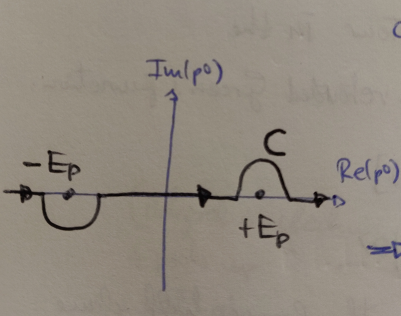
\includegraphics[width=0.3\linewidth]{gfx/Contour1}
	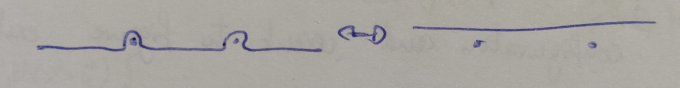
\includegraphics[width=0.7\linewidth]{gfx/Contour2}
	\caption{\itshape Integration contour for Feynman propagator of the real scalar field.}
	\label{fig:contour1}
\end{figure}
with $p^0$ integration along the real axis and with the limit $\epsilon \rightarrow 0$ after performing the integral.
The $i\epsilon$ term represents time ordering. Important is only the position of the poles with respect to the contour, thus the relative position.

\subsubsection{Propagators as Green's functions}
The Feynman propagator $D_F(x-y)$ is a Green's function for the Klein-Gordon equation:
\begin{equation}
	(\partial^2_x + m^2) D_F(x-y) = -i \delta^{(4)}_D(x-y).
\end{equation}
\begin{enumerate}
		\item
		\begin{figure}[h]
			\centering
			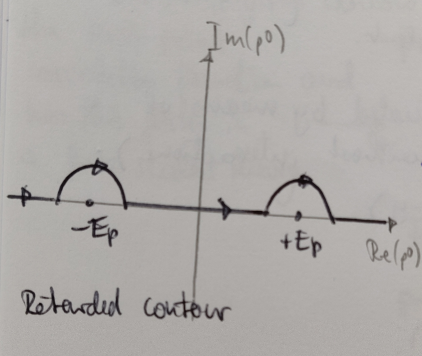
\includegraphics[width=0.7\linewidth]{gfx/Retardedcontour}
			\caption{\itshape Retarded contour.}
			\label{fig:retardedcontour}
		\end{figure} 
	 By avoiding both poles along a contour in the upper half-plane, the solution is the retarded Green's function
		\begin{equation}
			D_R(x-y)=\theta(x^0-y^0) [D(x-y)-D(y-x)]\equiv \theta(x^0-y^0) \expval{[\phi(x),\phi(y)]}{0}.
		\end{equation}
$D_R$ is useful in classical field theory if we know the initial value of some field configuration and want to figure out what it evolves into in the presence of the source.
It propagates information backward in time.
\item 
\begin{figure}[h]
	\centering
	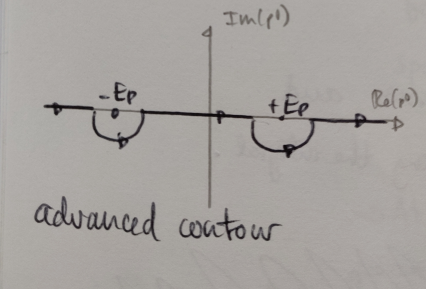
\includegraphics[width=0.7\linewidth]{gfx/Advancedcontour}
	\caption{\itshape Advanced contour.}
	\label{fig:advancedcontour}
\end{figure}
Avoiding both poles $p^0 = \pm \sqrt{E^2_{\vec{p}}}$ in the lower half plane yields the advanced Green's function
\begin{equation}
	D_A (x-y) = \theta(y^0-x^0) [D(x-y)-D(y-x)].
\end{equation}
$D_A$ is useful if we know the end point of a field configuration and want to figure out were it came from. It propagates forward in time.
\item $D_F(x-y)$ propagates positive frequency modes $e^{- i px}$ forward in time and negative frequency modes $e^{ipx}$ backward in time.
\end{enumerate}
\subsubsection{How to perform the contour integral}
Define a function $g(z)$ with poles $z_0$ and apply Residue theorem:
\begin{equation*}
	g(z) =\frac{1}{E_p+z} e^{-i z (x^0-y^0)}, \quad z_0 =E_p, z=p^0.
\end{equation*}
\begin{align*}
	\Rightarrow \theta(x^0-y^0)&=g(z_0)=\theta(x^0-y^0) \left[\frac{1}{2 \pi i} \oint_{C_1} \frac{g(z) \md z}{z-z_0}\right]\\
	&=\theta(x^0-y^0) \left[\frac{1}{2 \pi i}\oint_{C_1} \left(\frac{1}{E_p+p^0} e^{-i p^0 (x^0-y^0)} \right) \frac{\md p^0}{p^0-E_p}\right] \\
	&= \theta(x^0-y^0) \left[\frac{1}{2 \pi i} \oint_{C_1} \md p^0 \frac{e^{-i p^0(x^0-y^0)}}{(p^0+E_p)(p^0-E_p)}\right] \\
	&=-\theta(x^0-y^0) \frac{1}{2 \pi i} \oint_C \md p^0 \quad \frac{e^{-ip^0(c^0-y^0)}}{(p^0 + E_p)(p^0-E_p)},
\end{align*}
where the minus comes about since the integral is performed clockwise ($\Rightarrow \times (-1)$) and because it picks up the pole at $+E_p \Rightarrow (-1) \times (+1)=-1$.\\
\begin{align*}
	\theta(y^0-x^0) \frac{1}{2 E_p} e^{i E_p (x^0-y^0)} &= \theta(y^0-x^0) g(z_0) \\
	&=\theta(y^0-x^0) \left[\frac{1}{2 \pi i} \oint_{C_2} \left(\frac{1}{p^0+E_p} e^{-i p^0 (x^0-y^0)} \right) \frac{\md p^0}{p^0-E_p}\right] \\
	&= - \theta(y^0-x^0) \frac{1}{2 \pi i} \oint_{C_2} \md p^0 \quad \frac{e^{-i p^0(x^0-y^0)}}{(p^0+E_p)(p^0-E_p)},
\end{align*}
where the minus sign comes about since the integral is performed counter-clockwise ($\Rightarrow \times +1$) and because it picks up pole at $-E_p \Rightarrow +1 \times (-1)=-1$. Thus, the Feynman propagator is given by the addition of both contours
\begin{align*}
	D_F(x-y) &= \int \pmeasure e^{i \vec{p}(\vec{x}-\vec{y})} \left[-\theta(x^0-y^0) \frac{1}{2 \pi i} \oint_{C_1} \md p^0 \frac{e^{-i p^0(x^0-y^0)}}{(p^0+E_p)(p^0-E_p)} \right.\\
	&\left. \qquad - \theta(y^0-x^0) \frac{1}{2 \pi i} \oint_{C_2} \md p^0 \frac{e^{-i p^0(x^0-y^0)}}{(p^0-E_p)(p^0+E_p)}\right]\\
		&\stackrel{R\rightarrow\infty}{=} - \oint \frac{\md^4 p}{(2 \pi)^4} \frac{1}{i} e^{-i p\cdot (x-y)} \underbrace{\left[\theta(x^0-y^0)+\theta(y^0-^0)\right]}_{=1} \frac{1}{(p^0+E_p)(p^0-E_p)} \\
		&= \oint \frac{\md^4 p}{(2 \pi)^4} \underbrace{\frac{i e^{-i p\cdot(x-y)} }{(p^0+E_p)(p^0-E_p)}}_{=p^2-m^2}.
\end{align*}




\newpage





\section{Interacting scalar theory}
\subsection{Introduction}
Our consideration of free scalar field theories showed, that the theory is \emph{exactly solvable}, we can determine the spectrum (Hilbert space is the Fock space of multi-particle states created from the vacuum $\ket{0}$) and the fields have particle excitations which do not interact.\\
\\
Interactions are described in QFT by potentials $V(\phi)$ beyond quadratic order
\begin{equation}
	V(\phi) = \underbrace{\half m^2_0 \phi^2}_{V_0 (\phi)} \qquad + \sum_{n\geq 3} \frac{\lambda_n}{n!} \phi^n.
\end{equation}
The coefficients $\lambda_n$ are called \emph{coupling constants}. Here we restrict ourselves to
\begin{equation}
V(\phi) = \half m^2_0 \phi^2 +\underbrace{\frac{1}{3!} g \phi^3+\frac{1}{4!} \lambda \phi^4}_{V_{\mathrm{int}}},\quad [\lambda_n]=4-n \neq 0 !,
\end{equation}
with the decomposition 
\begin{equation}
	\mathcal{L}=\mathcal{L}_0 +\mathcal{L}_{\mathrm{int}},\quad \mL_{\mathrm{int}}=-V_{\mathrm{int}}, \quad  \mL_{\mathrm{int}}=-\mathcal{H}_{\mathrm{int}},\; H=H_0 +H_{\mathrm{int}}.
\end{equation}
\\
\\
Introducing interaction terms leads to changes in the theory:\\
\begin{enumerate}
	\item The Hilbert space is different from the free theory
	\begin{enumerate}
		\item $\ket{0}\leftrightarrow$ vacuum of $H_0:\quad H_0\ket{0} =E_0 \ket{0}$.\\
		  $\ket{\Omega}\leftrightarrow$ vacuum of $H:\quad H\ket{\Omega}=E_{\Omega} \ket{\Omega}$
		with $\ket{\Omega}\neq \ket{0}$ in general.
		\item The mass of the momentum eigenstates of $H$ does no longer equal the parameter $m_0$ that appear in $\mL_0$.
		\item Bound states (e.g. hydrogen) may exist in the spectrum.
		\end{enumerate}
	\item The states interact.
\end{enumerate}
The coupling constants are characterized as follows:
\marginpar{Only doing weakly coupled field theories here, because they can be considered as small perturbation of free field theory.}
\begin{enumerate}
	\item $[\lambda_3=g]=1$: The dimensionless parameter is $\lambda_3/E$, $E$ being the energy scale of the process of interest. This means that $\lambda_3 \frac{\phi^3}{3!}$ is a small perturbation at high energies $E\gg \lambda_3$, but a a large perturbation at low energies $E\ll \lambda_3$. Terms that we add to the Lagrangian with this behaviour are called \emph{relevant} because they are most relevant at low energies.
	\item $[\lambda_4=\lambda]=0$: This term is small if $\lambda_4 \ll 1$. Such perturbations are called \emph{marginal}. If $\lambda_4 \ll1$ then perturbation theory is applicable.
	\item $[\lambda_n]<0$ for $n\geq 5$: The dimensionless parameter is $(\lambda_n E^{n-4})$, which is small at low-energies and large at high energies. Such perturbations are called \emph{irrelevant}.
	\item Of the infinite number of interaction terms that we could write down, only $g$,$\lambda$ are needed (for real scalar field, else some more), because the irrelevant couplings become small at low-energies, our field of interest.
\end{enumerate}
\marginpar{Exact solution of non-free QFT is often not possible.}


\subsection{Källén-Lehmann spectral representation}
Here we take a look at the spectrum of an interacting real scalar field theory in a manner valid for all types of interactions and without relying on perturbation theory. This representation gives a \emph{general expression} for the time ordered two-point function of an interacting quantum field theory as a sum of free propagators.\\
In interacting theory $[H,\vec{P}]=0$ still holds due  to Lorentz invariance. Their mutual eigenstates $\ket{\lambda_p}$ with
\begin{equation}
	H\ket{\lambda_p}=E_p(\lambda) \ket{\lambda_p}, \quad \vec{P}\ket{\lambda_p} = \vec{p} \ket{\lambda_p}
\end{equation}
correspond via a Lorentz boost to the state at rest, called $\ket{\lambda_0}$.\\
\begin{figure}
	\centering
	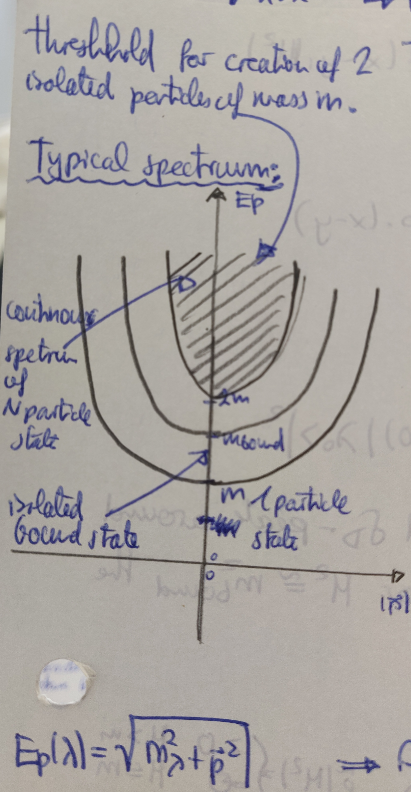
\includegraphics[width=0.7\linewidth]{gfx/Spectruminteractingtheory}
	\caption{\itshape Typical spectrum in the interacting theory.}
	\label{fig:spectruminteractingtheory}
\end{figure}
We can have the following types of $\ket{\lambda_{\vec{p}}}$:
\begin{enumerate}
	\item 1-particle states with $E^2_p = \vec{p}^2+m^2$, they have $p^{\nu}p_{\nu}=m^2$, $m\neq m_0$ (even in vacuum $m \neq m_0$ because of self-interactions).
	\item Bound states with no analogue in the free theory.
	\item 2-and $N$-particle states formed out of 1-particle and the bound states. In this case, we take $\vec{p}$ to the centre-of-mass momentum of the multi-particle state.
\end{enumerate}
All these are created from the vacuum $\ket{\Omega}$. The crucial difference to the free theory is, that $ \phi(x)$ cannot simply be written as a superposition of its Fourier amplitudes $a(\vec{p})$ and $a^{\dagger}(\vec{p})$, because $\phi(x)$ \emph{does not obey the free e.o.m}, rather 
\begin{equation}
	(\partial^2+m^2)\phi = j.
\end{equation}
Thus, acting with  $\phi$ on $\ket{\Omega}$ \emph{does not} simply created a 1-particle state as in the free theory!
\\
\\
\emph{Completeness relation} of this Hilbert space:
\begin{equation}
	\mathcal{I}=\ket{\Omega}\bra{\Omega} + \sum_{\lambda} \int \pmeasure \frac{1}{2 E_p(\lambda)} \ket{\lambda_p} \bra{\lambda_p},
\end{equation}
where $E_p(\lambda)=\sqrt{m^2_{\lambda}+\vec{p}^2}$ and $\sum$ includes a sum over 1-particle states, over all types of bound states as well as over all multiparticle states. $\int \md^3 p \dots$ refer to the centre-of-mass momentum of a state of species $\lambda$.\\
\\
\begin{mybox}{Feynman-propagator in interacting scalar theory}
We find the time-ordered interacting Feynman-propagator to be
\begin{equation}
\expval{T\phi(x)\phi(y)}{\Omega} = \sum_{\lambda} \int \frac{\md^4 p}{(2 \pi)^4} \frac{i}{p^2-m^2_{\lambda} +i\epsilon} e^{- i \cdot (x-y)} |\bra{\Omega}\phi(0)\ket{\lambda_0}|^2,
\end{equation}
or rather in the Kallén-Lehmann spectral representation
\begin{equation}
	\expval{T\phi(x)\phi(y)}{\Omega} = \int_0^{\infty} \frac{\md M^2}{2 \pi} \quad \rho(M^2) D_F(x-y,M^2),
\end{equation}
where we defined
\begin{equation}
	D_F(x-y, M^2) = \int \frac{\md^4 p}{(2 \pi)^4} \frac{i}{p^2-M^2+i\epsilon} e^{-i p\cdot (x-y)} 
\end{equation}
and the \emph{spectral function} (density)
\begin{equation}
	\rho(M^2) = \sum_{\lambda} 2 \pi \delta_D(M^2-m^2_{\lambda}) |\bra{\Omega} \phi(0) \ket{\lambda_0}|^2.
\end{equation}
\end{mybox}
\begin{figure}
	\centering
	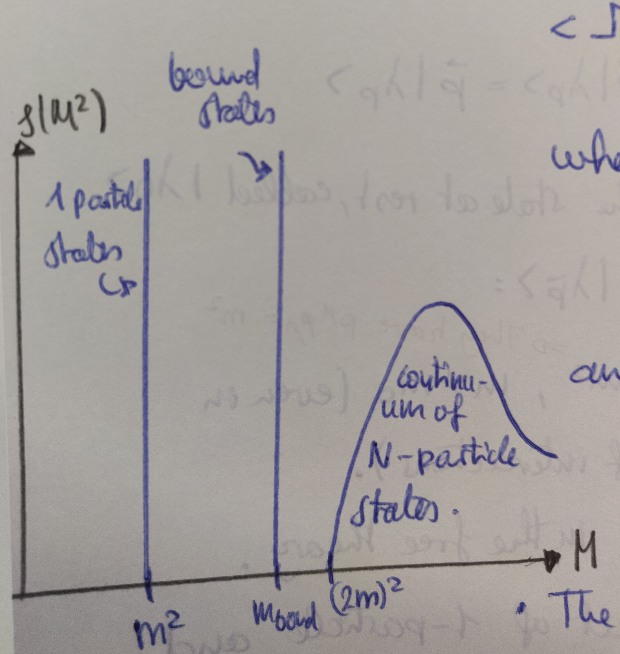
\includegraphics[width=0.7\linewidth]{gfx/SpectrumInteractingTheoryMass}
	\caption{\itshape Particle spectrum with respect to the mass.}
	\label{fig:spectruminteractingtheorymass}
\end{figure}
The 1-particle state lead to an isolated $\delta_D$-peak around $M^2=m^2$. Therefore, below $M^2\approx(2m)^2$ or $M^2\approx m^2_{\mathrm{bound}}$ the spetral function takes the form
\marginpar{In general $\int_0^{\infty} \frac{\md M^2}{2 \pi} \rho(M^2)=1$ holds.}
\begin{align}
	\rho(M^2) &= 2 \pi \delta_D(M^2-m^2) \quad Z \\
	&= 2 \pi \delta_D(M^2-m^2) Z+ \tilde{\rho}(M^2), \quad \tilde{\rho} (M^2) \left\{ \begin{array}{lr} \geq 0 & M>m \\
		=0 & M \leq m.
	\end{array}\right\}
\end{align}
with the \emph{wavefunction renormalization} $Z$ which takes as a rescale factor the effects of interactions or quantum fields into account
\begin{equation}
	Z=|\bra{\Omega}\phi(0)\ket{1_0}|^2,
\end{equation}
where $\ket{1_0}$ is the 1-particle state at rest.
\\
\\
We find the following statements 
\begin{enumerate}
	\item
	\marginpar{Calculation of the propagator yields the mass of the particle !}  The 1-particle state is the first analytic pole of the fully Feynman propagator at $m^2 \Rightarrow$ The mass-square $m^2$ of the particle is the location of the lowest-lying pole of the Fourier transformed propagator.
	\item Bound states appear at higher isolated poles
	\item N-particle states give rise to a branch cut beginning at $p^2=em^4$.
\end{enumerate}
The field strength renormalization in a free theory, i.e. $Z=1$, because $\phi(0)$ just creates the free particle from vacuum. In an interacting theory
\begin{equation}
	1 > \sqrt{Z} = \quad |\bra{\Omega} \phi(0) \ket{1_0}|,
\end{equation}
because $\phi$ creates not only 1-particle states and thus the overlap with the 1-particle states is smaller. Thus,
\begin{statements}
	$Z=1$ if and only if the theory is free.
\end{statements}
In the derivation of the interacting Feynman propagator we made use of the transformation behaviour of a scalar field under a Lorentz transformation
\begin{equation}
	x \mapsto x'=\Lambda x \quad \Rightarrow \quad U^{-1}(\Lambda)\phi(x') U(\Lambda) = \phi(x),
\end{equation}
because classically $\phi(x) \mapsto \phi'(x')=\phi(x)$ has its analogue in 
\begin{equation}
	\Leftrightarrow \bra{\alpha'} \phi(x') \ket{\beta'} = \bra{\alpha} \phi(x)\ket{\beta}=\bra{\alpha}U^{-1} \phi(x')U\ket{\beta}.
\end{equation}


\subsection{S-matric and asymptotic in/out-states}
\marginpar{Can be drrived in the interaction picture as well, but here with in \& out states.}
Consider scattering of incoming states $\ket{\alpha,in}$ to outgoing states $\ket{\beta,out}$ with the aim of computing the QM transition amplitude, i.e. the probability amplitude for scattering of $\ket{\alpha,in}$ to $\ket{\beta,out}$.
\begin{mybox}{In and out states}
	Associated to the in and out states are the in and out field operators $\phi_{in}, \phi_{out}$, which satisfy
	\begin{equation}
		(\partial^2+\underbrace{m^2}_{\neq m^2_0}  \phi_{in, out} (x) = 0 !!.)
	\end{equation}
	They have the same equal time commutation relations
	\begin{equation}
		[\phi_{in, out}(x),\Pi_{in,out} (y)]_{x^0=y^0} = i \delta^{(3)}_D (\vec{x}-\vec{y}),
	\end{equation}
	with others vanishing.
\end{mybox}
Associated to the in and out fields are two sets of creation and annihilation operators, $a^{\dagger}_{in}(\vec{p}), a_{in}(\vec{p}), a^{\dagger}_{out}(\vec{p}),a_{out}(\vec{p})$, acting in the same Hilbert space, on two complete sets (Fock spaces, initial $\mathcal{F}_{in}$ and final space $\mathcal{F}_{out}$). These operators satisfy the commutation relations
\begin{equation}
	[a_{in,out}(\vec{p}) , a^{\dagger}_{in,out} (\vec{p})]= i \delta_D(\vec{p}-\vec{p}'),
\end{equation}
with others vanishing.\\
The action of the creation operators on the respective vacua and states with a finite number of particles in the in and out states is given by
\begin{align}
	\ket{in, q_1, \dots,q_n} &=a^{\dagger}_{in}(\vec{q}_1) \dots a^{\dagger}_{in} (\vec{q}_n) \ket{\Omega,in}\\
	\ket{p_1,\dots, p_n, out} &= a^{\dagger}(\vec{p}_1) \dots a^{\dagger}(\vec{p}_n) \ket{\Omega,out}\\
	\mathcal{H}_i &= \mathrm{span}\{\ket{in, q_1,\dots, q_n}\}\\
	\mathcal{H}_f &= \mathrm{span}\{\ket{out,p_1,\dots,p_n}\},
\end{align}
where issues of normalization have been ignored!
\begin{mybox}{Relation between free vacuum $\ket{0}$ and interacting vacuum$\ket{\Omega}$}
		\begin{equation}
			\ket{0,in}=\ket{0,out} = \ket{\Omega}.
		\end{equation}
\end{mybox}
In the \emph{asymptotic past}, $t\rightarrow-\infty$, the in-states $\ket{i, in}$ are described as distinct wave packets corresponding to well-separated single particle states. Being far apart for $t\rightarrow-\infty$, they travel freely as individual states.\\
As these states approach each other, they start to interact and scatter into the final states. For $t\rightarrow\infty$ these final states are again asymptotically free and well-separated 1-particle states.\\
\\
We can expand
\begin{equation}
	\phi_{in}(x) = \int \pmeasure \frac{1}{\sqrt{2 E_p}} \left[a_{in}(\vec{p}) e^{- i p\cdot x} +a^{\dagger}_{in} (\vec{p}) e^{i p\cdot x}\right].
\end{equation}
We can identify
\begin{equation}
	\lim_{t\rightarrow - \infty} \bra{\alpha}\phi\ket{\beta} = \lim_{t\rightarrow - \infty} \sqrt{Z} \bra{\alpha}\phi_{in} \ket{\beta} \; \Leftrightarrow\; \begin{array}{lr}
	\bra{\alpha}\phi \ket{\beta} \stackrel{t \rightarrow - \infty}{\rightarrow} \sqrt{Z} \bra{\alpha}\phi_{in} \ket{\beta} \\
	\bra{\alpha}\phi \ket{\beta} \stackrel{t\rightarrow +\infty}{\rightarrow} \sqrt{Z} \bra{\alpha} \phi_{out} \ket{\beta}
	\end{array}.
\end{equation}
\subsubsection{The S-matrix and the scattering process}
\begin{mybox}{The S-matrix}
	The S-matrix (scattering) maps the out-states onto the in-states (because the Fock spaces are isomorphic):
	\begin{equation}
		\ket{\alpha, in} = \quad S\ket{\alpha, out},
	\end{equation}
	with the properties
	\begin{enumerate}
		\item S is unitary $S^{\dagger} = S^{-1}$,
		\item $\phi_{in}(x) = \quad S \phi_{out}(x) S^{-1}$,
		\item $\ket{vac, in} =\ket{vac, out} = \ket{\Omega}$ and $S\ket{\Omega}=\ket{\Omega}$.
	\end{enumerate}
Thus, 
\begin{equation}
|\bra{f,in}S\ket{i,in}|^2 
\end{equation}
\emph{is the probability for scattering from initial states to the final states !}.
\end{mybox}
Formally, the scattering process is described  by the following:
We have one Hilbert space for the whole scattering process from $t=-\infty$ to $t=+\infty$. There exist two Fock spaces $\mathcal{F}_{in}, \mathcal{F}_{out}$ in this Hilbert space, they are not disjoint because states can simply not participate in the scattering process. Long before the collisions, i.e. in the asymptotic past, we have well separated, free and independent wavepackets, the $\ket{\alpha,in}$ states with $\mathcal{F}_{in}=\mathrm{span}\{\ket{\alpha,in}\}$. Long after the collisions, we again have well separated, free and independent wavepackets, the $\ket{\beta,out}$ states with $\mathcal{F}_{out} = \mathrm{span}\{\ket{\beta,out}\}$. Then there exists an isomorphism between $\ket{\alpha,in}$ and $\ket{\beta,out}$, the $S$-matrix, with
\marginpar{$\mathcal{H}=\mathcal{F}_{out} \cup \mathcal{F}_{in}, \mathcal{F}_{out} \cap \mathcal{F}_{in} \neq \emptyset$.}
\begin{equation}
	\ket{\alpha, in}=S\ket{\alpha,out}, \qquad S:\mathcal{F}_{out} \rightarrow \mathcal{F}_{in}.
	\end{equation}
Then again, $\mathcal{F}_{in}=\mathrm{span}\{\ket{\alpha,in} = \phi_{in}(x)\ket{\Omega,in}\}$ and $\mathcal{F}_{out}=\mathrm{span}\{\ket{\beta,out}= \phi_{out}(x) \ket{\Omega,out}\}$ with $\ket{\Omega,in} = \ket{\Omega,out}=\ket{\Omega}$.\\
We thus find
\begin{align}
	S_{\beta \alpha} &:= \braket{\beta,out}{\alpha,in}, \qquad \ket{\alpha,in} = \sum_{\beta} S_{\beta \alpha} \ket{\beta,out}\\
	\Rightarrow \hat{S}\ket{\alpha,out} &=\sum_{\beta} S_{\beta \alpha} \ket{\beta,out} = \ket{\alpha,in} \\
	\Rightarrow S_{\beta \alpha} &= \braket{\beta,out}{\alpha,in} = \bra{\beta,out} \hat{S}\ket{\alpha,out}\\
	\bra{\beta,out}S^{\dagger} &= \bra{\beta,in} \qquad SS^{\dagger}=\sum_{\beta} \ket{\beta,in}\bra{\beta,in} = \mathcal{I}.
\end{align}
The probability amplitude for scattering from initial to final state.

\subsection{The LSZ reduction formular}
\marginpar{As it is always the case for in and out states we regard the fully interacting theory, $\ket{\Omega}$.}
\begin{mybox}{The LSZ reduction formular}
The aim is to compute a S-matrix element $\braket{p_1,\dots,p_n,out}{q_1,\dots,q_r,in}$ for a real scalar field. Note that $p_1,\dots,p_n$ and $q_1,\dots,q_r$ are \emph{on-shell} since they correspond to the physical 4-momentum of the out-and incoming 1-particle states. We find

\begin{align*}
	&\braket{p_1,\dots,p_n,out}{q_1,\dots,q_r,in}= \bra{p_1,\dots,p_n, in}S\ket{q_1,\dots,q_r,in} \\
	&= (\sum \mathrm{disconnected \;terms}) +(i Z^{-\half})^{n+r} \int \md^4 y_1 \dots \md^4 y_n\\
	& \int \md^4 x_1 \dots \md^4 x_r \exp\left\{i\left[\sum_{k=1}^{n} p_k \cdot y_k - \sum_{l=1}^{r} q_l \cdot x_l\right]\right\} \\
	&\times (\partial^2_{y_1} + m^2) \dots (\partial^2_{x_1} +m^2) \\
	&\expval{T\phi(y_1) \dots \phi(y_n) \phi(x_1)\dots \phi(x_n)}{\Omega}..
\end{align*}
\end{mybox}
\marginpar{
	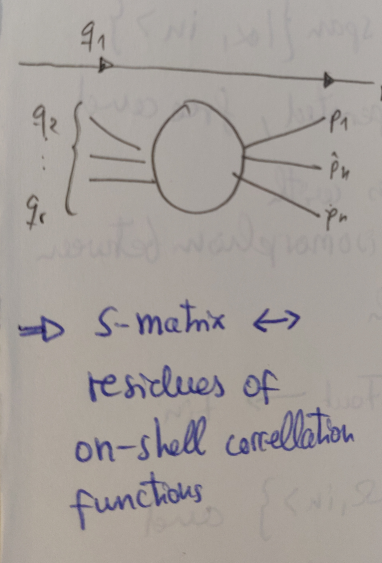
\includegraphics[width=0.3\marginparwidth]{gfx/disconnectediagram}
	\captionof{figure}{\itshape Disconnected diagram}
		\label{fig:disconnectediagram}
}
This LSZ-formula reduces the computation of the S-matrix to the computation of time-ordered correlation functions\\ $\expval{T\phi(y_1) \dots \phi(y_n) \phi(x_1)\dots \phi(x_n)}{\Omega}$ of the full interacting theory.\\
The first term describes a process where on of the in-and outgoing states are identical and do not participate in scattering.
Such an amplitude corresponds to a disconnected diagram, compare fig. \ref{fig:disconnectediagram}, and its computation reduces to computing an S-matrix element involving only $(r-1)$ in-and $(n-1)$ out-states.\\
For the connected term we find
\begin{align*}
	&\prod_{k=1}^{n} \int_{\mR^{3,1}} \md^4y_k e^{i p_k \cdot y_k} \prod_{l=1}^{r} \int_{\mR^{3,1}} \md^4x_l e^{-i q_l \cdot x_k}  \times \expval{T\prod_k \phi(y_k) \prod_l \phi(x_l)}{\Omega}\\
	&= \left(\prod_{k=1}^n \frac{i \sqrt{Z}}{p^2_k-m^2}\right) \left(\prod_{l=1}^{r} \frac{i \sqrt{Z}}{q^2_l - m^2}\right) \times \bra{p_1,\dots,p_n}S\ket{q_1,\dots,q_r}  |_{\mathrm{connected}}.
\end{align*}
\begin{statements}
	S-matrix $\leftrightarrow$ residues of on-shell correlation functions.
\end{statements}
$\expval{T\tilde{\phi}(p_1) \dots \tilde{\phi}(p_n) \tilde{\phi}(q_1)\dots \tilde{\phi}(q_r)}{\Omega} $ will in general be a sum of terms with different poles in the momenta. Only the term with the pole structure given precisely by $\prod_{k=1}^{n} \frac{1}{p^2_k - m^2} \prod_{l=1}^{r} \frac{1}{q^2_l-m^2}$ contributes to the connected S-matrix element.



\subsection{Correlators in the interaction picture}
The computation of the full correlator shall now be reduced to a calculation in terms of free-field creation/annihilation operators and the free-field vacuum. This is achieved in the interaction picture: 
	\marginpar{$H=H_0+H_{int}$, $[H_0,H]\neq 0$.}
\begin{mybox}{Operator fields in the interaction picture}
	The time dependence of operators in governed by $H_0$, while the time dependence of states is governed by $H_int$:
	\begin{align}
		\phi_I(t,\vec{x}) &= e^{i H_0 (t-t_0)} \phi(\vec{x},t_0) e^{-i H_0 (t-t_0)} \\
		\Pi_I(t,\vec{x}) &= e^{i H_0 (t-t_0)} \Pi(\vec{x},t_0) e^{-i H_0 (t-t_0)} \\
		\ket{\psi(t)}_I &= e^{i H_0 t} \ket{\psi(t)}_S \\
		H_I &\equiv (H_{\mathrm{int}})_I = e^{i H_0 t} (H_{\mathrm{int}})_S e^{-i H_0 t}.
	\end{align}
	Then $\phi_I(t,\vec{x})$ satisfies the free Klein-Gordon equation
	\begin{equation}
	(\partial^2+m^2_0) \phi_I(t,\vec{x}) = 0,
	\end{equation}
	thus a \emph{free mode expansion} is possible.
\end{mybox}
The free mode expansion reads
\begin{equation}
\phi_I(x) = \int \pmeasure \frac{1}{\sqrt{2 E_p}} \left[a_I(\vec{p}) e^{-i p\cdot x} + a^{\dagger}_I(\vec{p}) e^{i p\cdot x} \right]
\end{equation}
with
\begin{equation}
[\phi_I(t,\vec{x}), \Pi_I(t,\vec{y})]=i \delta^{(3)}_D(\vec{x}-\vec{y}), \quad [a_I(\vec{p}),a^{\dagger}_I(\vec{q})] = (2 \pi)^3 \delta^{(3)}_D(\vec{p}-\vec{q}).
\end{equation}
Therefore the results of the free theory carry over:
\begin{equation}
H_= \ket{0}=0, \qquad a_I(\vec{p})\ket{0}=0.
\end{equation}
The transition to Heisenberg picture can now be done with
\begin{equation}
\phi(t,\vec{x}) = U^{\dagger}(t,t_0)  \phi_I(t,\vec{x}) U(t,t_0)
\end{equation}
with the time-evolution operator
\begin{equation}
U(t,t_0) = e^{i H_0(t-t_0)} e^{-i H(t-t_0)} = \hat{T}e^{-i \int_{t_0}^{t} H_I(t') \md t'}.
\end{equation}
\begin{mybox}{How to compute the correlators}
	The logic is now to replace the Heisenberg picture operators $\phi(x)$ om the correlator $\expval{T\phi(y_1) \dots \phi(y_n) \phi(x_1) \dots \phi(x_r)}{\Omega}$ by the interaction picture operators $\phi_I(x)$ because they obey a \emph{free mode expansion}.\\
\end{mybox}
We find \emph{Dyson's formula} for the time-evolution operator
\begin{align}
	U(t,t_0) &= \mathcal{I} + \sum_{n=1}^{\infty} \left(\frac{1}{i}\right)^n \int_{t_0}^{t} \md t_1 \int_{t_0}^{t_1} \md t_2 \dots \int_{t_0}^{t_{n-1}} \md t_n \underbrace{H_I(t_1)H_I(t_2)\dots H_I(t_n)}_{\mathrm{these \, are\, time-ordered}}\\
	&= \sum_{n=0}^{\infty} \frac{(-i)^n}{n!} \int_{t_0}^{t}\md t_1 \int_{t_0}^{t} \md t_2 \dots \int_{t_0}^{t} \md t_n T H_I (t_1)H_I(t_n) \\
	&=T e^{-i \int_{t_0}^{t} \md t'H_I(t')}.
\end{align}
With the properties
\begin{align}
	U^{\dagger}(t_1,t_2) &=U^{-1}(t_1,t_2) = U(t_2,t_1) \\
	U(t_1,t_2)U(t_2,t_3) &= U(t_1,t_3) \quad \mathrm{for} \quad t_1 \geq t_2 \geq t_3.
\end{align}
There is an equivalent representation of the time-evolution operator
\begin{align}
	U(t) &= \lim_{n\rightarrow \infty} \left\{  \left[1-i H_{I,int} (\tau_{n-1}) (\tau_n - \tau_{n-1})\right] \right. \\
	&\left.\left[1-i H_{I,int}(\tau_{n-2}) (\tau_{n-1}-\tau_{n-2}) \right]\dots \left[1-iH_{I, int} (\tau_0) (\tau_1-\tau_0) \right]   \right\}.
\end{align}
\\
\\
Furthermore we find a relation between the free vacuum $\ket{0}$ and the interacting vacuum $\ket{\Omega}$. The time-evolution of the free vacuum is
\begin{equation}
	e^{-iHT} \ket{0} = e^{-iHT} \sum_{\ket{n}} \ket{n} \braket{n}{0} = e^{- iE_{\Omega}T} \ket{\Omega}\braket{\Omega}{0}+\sum_{\ket{n} \neq \ket{\Omega}} e^{-iE_n T}\ket{n}\braket{n}{0}.
\end{equation}
The idea is, that the second term must vanish for $T\rightarrow \infty$, because excited states will go down eventually.\\
If $H_0 \ket{0}=0$, then $H\ket{\Omega} =E_{\Omega}\ket{\Omega}$ with $E_{\Omega}\neq 0$ and $E_n > E_{\Omega} \forall \ket{n} \neq \ket{\Omega}$. So if we formally take the limit $T\rightarrow\infty(1-i\epsilon)$, then $e^{-i E_n T}$ is stronger suppressed and only the vacuum $\ket{\Omega}$ survives:
\begin{align}
	\ket{\Omega} &= \lim_{T\rightarrow\infty(1-i\epsilon)} \left[e^{-i E_{\Omega} (t_0 - (-T)) \braket{\Omega}{0}}\right]^{-1} U(t_0,-T) \ket{0} \\
	\Rightarrow \expval{\hat{T}\phi(x) \phi(y)}{\Omega} &= \lim_{T\rightarrow \infty(1-i \epsilon)} \frac{\expval{\hat{T} \left(\phi_I(x) \phi_I(y) e^{-i \int_{-T}^{T} \md t H_I(t)} \right)}{0}}{\expval{\hat{T} e^{-i \int_{-T}^{T} \md t H_I(t)}}{0}}
\end{align}
with the same reasoning for higher n-point correlators.\\
Thus, gauge $E_0$ energy to be zero: $H_0 \ket{0}=E_0 \ket{0}=0$ such that $H\ket{\Omega} =E_{\Omega} \ket{\Omega} \neq 0$.
\begin{mybox}{Logic on how to compute correlators}
	Replace Heisenberg with interaction picture operators, from this we get $e^{-i \hbar \int H_I}$. Then go over from $\ket{\Omega}\rightarrow\ket{0}$ with given relation. Then compute $\expval{\phi \dots \phi}{0}$ explicitly via Wick normal ordering $\Rightarrow$ express results in terms of Feynman diagrams.
\end{mybox}



\subsection{Wick's Theorem}
From Dyson's formula, we want to compute quantities like $\bra{f}T[H_I(x_1)\dots H_I(x_n)] \ket{i}$, where $\ket{i}$ and $\ket{f}$ are eigenstates of the free theory. Since the $H_I$'s contain certain creation and annihilation operators, calculation would be way easier if all annihilation operators were ordered to the right.
\begin{mybox}{Normal ordering}
	An operator $O$ is \emph{normal-ordered} if all creation/annihilation operators appear on the left/right. For such $O$ we write $:O:$.
	\begin{equation}
		\Rightarrow \expval{\normord{O}}{0} = 0
	\end{equation}
	for every non-trivial operator $O\neq c \mathcal{I}, c\in \mathbb{C}$.
\end{mybox}
\begin{mybox}{Contraction}
	\begin{equation}
		\contraction{}{\phi_I(x)}{}{\phi_I(y)} \phi_I(x) \phi_I(y) := D^{(0)}_F (x-y) = D^{(0)}_F(y-x)
	\end{equation}
	with the free Feynman propagator
	\begin{equation}
		D^{(0)}_F(x-y) =\oint_C \frac{\md^4p}{(2 \pi)^4} \frac{i}{p^2-m^2_0} e^{i p\cdot (x-y)}.
	\end{equation}
\end{mybox}
\begin{mybox}{Wick's theorem}
	We can formulate Wick's theorem now
	\begin{align*}
		&\hat{T}\phi_I(x_1) \dots \phi_I(x_n) \\
		&= \normord{\phi_I(x_1) \dots \phi_I(x_n)} + \normord{all \,contractions\, of \,distinct\, pairs} \\
				&= \normord{\phi_I(x_1) \dots \phi_I(x_n)} + \sum_{i<j} \contraction{}{\phi_I(x_i)}{}{\phi_I(x_j)} \phi_I(x_i) \phi_I(x_j) \\
				&\normord{\phi_I(x_1) \dots \phi_I(x_{i-1})\phi_I(x_{i+1}) \dots  \phi_I(x_{j-1}) \phi_I(x_{j+1}) \dots \phi_I(x_n)} \\
				&+ \sum_{i<j, k<l} \contraction{}{\phi_I(x_i)}{}{\phi_I(x_j)} \phi_I(x_i) \phi_I(x_j) \contraction{}{\phi_I(x_k)}{}{\phi_I(x_l)} \phi_I(x_k) \phi(x_l) \\
				&\normord{\phi_I(x_1) \dots \phi_I(x_n)}+ \dots 
	\end{align*}
with $\normord{\contraction{}{\phi_1}{\phi_2}{\phi_3} \phi_1 \phi_2 \phi_3 \phi_4} \Leftrightarrow D^{(0)}_F(x_1-x_3) \normord{\phi_2 \phi_4}$.
\end{mybox}
\marginpar{Alternatively: $D^{(0)}_F(x-y) = \int_{\mR^{3,1}} \frac{\md^4p}{(2\pi)^4} \frac{i}{p^2-m^2_0 +i \epsilon} e^{- i p(x-y)}$.}
Wick's theorem has two important consequences
\begin{align}
	1) \expval{\hat{T} \phi_I(x_1) \dots \phi_I(x_{2N+1})}{0} &= 0 \quad \forall N\in \mathbb{N} \\
	2) \expval{\hat{T}\phi_I(x_1) \dots \phi_I(x_{2N})}{0} &=D^{(0)}_F(x_1-x_2) D^{(0)}_F(x_3-x_4) \\\nonumber
	&\dots D^{(0)}_F(x_{2N-1}-x_{2N}) \\ \nonumber
	& \sum (all \,other\, contractions).\nonumber
\end{align}
Therefore, Wick's theorem allows us to turn any expression of the form  
\begin{equation}
	\expval{\hat{T}\{\phi_I(x_1) \dots \phi_I(x_n)\}}{0}
\end{equation}
into a sum of products of Feynman propagators.\\
\\
\begin{mybox}{How to compute correlators}
	Correlation function in the full interacting theory $\mL = \mL_0 + \mL_{int}$:
	\begin{equation}
		\expval{\hat{T}\prod_{i=1}^{n} \phi(x_i)}{\Omega} = \frac{\expval{\hat{T} \prod_{i=1}^{n} \phi(x_i) e^{-i \int_{\mR^{3,1}} \md^4 x \mL_{int}}}{\Omega}}{\expval{\hat{T}e^{-i \int_{\mR^{3,1}} \md^4 x \mL_{int}}}{\Omega}}.
	\end{equation}
\end{mybox}

\subsection{Feynman diagrams}
There exists a graphical representation of the systematics of contractions in terms of Feynman diagrams. First introduce some definitions.
\begin{enumerate}
	\item The symmetry factors $S=|G|$ represent the order (Kardinalität) of the symmetry group of the diagrams.
	\begin{mybox}{Symmetry factors}
		The symmetry factors are given by the number of ways one can exchange components of the diagram without changing the diagram, where by components we mean either the two ends of a line starting and ending on the same point, entire lines between points or internal points.$\Rightarrow G\times \mathbb{Z}_2$ for every possible change $+$ the ones described in the following.
	\end{mybox}
It holds in general, that a Feynman diagram with symmetry group $G$ always carries a combinatorial factor $\frac{1}{|G|}$ This is because if some symmetry remains, the factor of $\frac{1}{n!}$ in the interaction term $\frac{- \lambda_n}{n!}\phi^n$ is only partially cancelled by counting the various contractions that yield the same diagram.
\begin{mybox}{How to calculate symmetry factors}
	In addition, if $k$ vertices are identical, the symmetry group includes the group of permutations of these $k$ vertices of order $|S_k|=k!$. One also has to take the symmetry group $S_k$ for $k$ lines between two connected vertices into account, e.g.
	
			\[
				\begin{gathered}
		\feynmandiagram [small, vertical=a to b, black] {
			a[particle=i] [dot]-- b [particle=j] [dot],
			a-- [half left]b ,
			b-- [half left]a ,
		};
	\end{gathered}
\quad \Rightarrow \quad S_3, |S_3|=3!.	\]
\end{mybox}
THe symmetry comes from the internal points, because the external points are distinct in their connections to the other points.
\item Number of pairings of $(2n)$ fields 
\begin{equation}
	\#= \frac{C^{2n}_2 C^{2n-2}_2 \dots C^2_2}{n!}, \quad C^n_m=\begin{pmatrix}
	n\\
	m
	\end{pmatrix}.
\end{equation}
Check the total number of fields you have found by this formula, to be correct. Or, equivalently for pairings of $n$ fields
\begin{equation}
	\# = \frac{(2n)!}{n! 2^n}.
\end{equation}
\item The \emph{$x,y$ associated to $\phi(x)\phi(y)$} in the correlator, which are not integrated over, are called \emph{external points}.
\item All other \emph{points over which is integrated over are called internal points.}
\item  \begin{mybox}{Vertices}
	For $\phi^n$ interaction, at an internal point $n$ lines meet. Such points are called \emph{vertices}.
\end{mybox}
\end{enumerate}

\subsubsection{Position space Feynman-rules}
In the following, rules are summarized for the computation of
\begin{equation}
	\expval{\hat{T} \left\{ \prod_{i=1}^{m} \phi_I(x_i) \exp\left[-i  \frac{\lambda}{n!} \int \md^4 z \phi^n_I(z) \right] 	\right\}}{0}
\end{equation}
at order $\lambda^k$, where we are assuming that all points $x_i$ are distinct:
\begin{enumerate}
	\item Draw one external point for all $x_i$ and $k$ internal points for all $z_j \cdot \left( \begin{array}{lr}
	i=1,\dots,m \\
	j=1,\dots,n
	\end{array}\right).$
	\item Connect the points by lines such that 
	\begin{enumerate}
		\item To each external point $x_i 1$ line is attached.
		\item To each internal point $z_j n$ lines are attached.
	\end{enumerate}
\item To each line between points $y_i$ and $y_j$ (both external and internal) we associate a free propagator
\begin{equation}
D^{(0)}_F(y_i - y_j) = D^{(0)}_F(y_j-y_i).
\end{equation}
\item To each vertex $z_j$ associate a factor
\begin{equation}
	-i \lambda \int \md^4z_j.
\end{equation}
\item To each external point associate a factor of 1.
\item Multiply all factors, Feynman propagators etc. and divide by the symmetry factor of the diagram.
\item Then sump up all distinct such Feynman diagrams.
\end{enumerate}


\subsubsection{Momentum space Feynman-rules}
The momentum-space Feynman rules for the computation of the $n$-point correlator at order $\lambda^k$
\begin{equation}
\expval{\hat{T} \left\{ \prod_{i=1}^{m} \phi_I(x_i) \exp\left[-i  \frac{\lambda}{n!} \int \md^4 z \phi^n_I(z) \right] 	\right\}}{0}
\end{equation}
are the following. This is an equivalent set of rules for the computation of the correlator where the integral over the vertex positions has been performed explicitly!
\begin{enumerate}
	\item Draw one external point for all $x_i$ and $k$ internal points $z_j$, $j=1,\dots,k$.
	\item Connect the points by lines such that
	\begin{enumerate}
		\item To each external point $x_i, 1$ line is attached.
		\item To each internal point $z_j, n$ lines are attached.
	\end{enumerate}
\item to each line between points $y_i$ and $y_j$ (both external and internal) we associate a free propagator 
\begin{equation}
	D^{(0)}_F(y_i-y_j)
\end{equation}
with one (arbitrary) choice of direction and to each such $D^{(0)}_F(y_i-y_j)$ we associate directed momentum $p$ from $y_i$ to $y_j$ and a factor
\begin{equation}
	\frac{i}{p^2-m^2_0+i \epsilon}.
\end{equation}
Note that 
\begin{align*}
	D^{(0)}_F (x-y) &= \int \frac{\md^4p}{(2 \pi)^4} \frac{i}{p^2-m^2_0+i \epsilon} e^{-i p(x-y)} \\
								&=\feynmandiagram [horizontal=a to b] {a[particle=x] -- [fermion] b[particle=y]}; \\
								&=\feynmandiagram [horizontal=b to a] {b[particle=y] --  [fermion]a[particle=x]};\\
						&=D^{(0)}_F (y-x).
\end{align*}
\item At each vertex, 4-momentum is conserved! For each vertex we thus multiply a factor of 
\begin{equation}
	(-i \lambda) \; (2 \pi)^4 \quad \delta^{(4)}_D \left(\sum_{ingoing} p_i - \sum_{outgoing} p_k\right).
\end{equation}
\item For each external point we multiply a factor of $e^{-i p\cdot x}$ for momentum pointing out of the external point ($
e^{- i p\cot x} =\feynmandiagram [horizontal=a to b] {a[particle=x] -- [fermion] b};$), or for momentum pointing into the point we multiply a factor $e^{+ i p \cdot x}$ ($e^{ i p\cot x} =\feynmandiagram [horizontal=a to b] {a -- [fermion] b[particle=x]};$).
\item Integrate over each momentum $\int \frac{\md^4 p}{(2 \pi)^4}$ and divide by the symmetry factor.
\item Then sum up all distinct such Feynman diagrams.
\end{enumerate}
\begin{mybox}{Summary of the calculation of Feynman diagrams}
	For example, the two-point correlator factorizes into connected and disconnected diagrams:
	\begin{align}
	&	\lim_{T\rightarrow \infty(1-i \epsilon)} \expval{\hat{T} \phi(x) \phi(y) e^{-i \int_{-T}^T \md t \; H_I(t)} }{0}\nonumber \\
	&= \sum(connected \, diagrams) \cdot e^{\sum(disconnected\, diagrams)}.
	\end{align}
	where the sum of connected diagrams is equal to
	\begin{equation}
		\sum(connected\,diagrams) = \feynmandiagram [horizontal=a to b] {a[particle=x] -- [fermion] b[particle=y]};
		+ \feynmandiagram [horizontal=a to b] {a[particle=x] -- c[particle=z],
			c--[fermion] b[particle=y],
		c -- [half left] c }; \dots
	\end{equation}

	the sum of at least partially connected diagrams with $n$ external points.\\
	And where $\sum$(disconnected terms) is equal to
	the sum of all entirely disconnected diagrams without external points.\\
	Such that
	\begin{align}
		\expval{\hat{T}\phi(x) \phi(y)}{\Omega} &= \lim_{T\rightarrow \infty(1-i \epsilon)} \frac{\expval{\hat{T}\phi(x) \phi(y) e^{-i \int_{-T}^T \md t \; H_I(t)} }{0}}{\expval{\hat{T} e^{-i \int_{-T}^T \md t \; H_I(t)} }{0}} \\
		&= \sum (connected \, diagrams) \\
		& = \dots 
	\end{align}

Or more generally
\begin{equation}
	\expval{\hat{T} \prod_{i=1}^{n} \phi(x_i) }{\Omega} = \sum^{\mathrm{over \, all \, partially \, connected}}_{\mathrm{diagrams\, with\, n\, external \, points}}.
\end{equation}
\end{mybox}
	\todo{Insert correct Feynman diagrams here from page 16.}




\subsection{Disconnected diagrams}
A typical diagram contains \emph{disconnected pieces}, i.e. subdiagrams which are not connected to any of the external points.\\
A disconnected piece contains only internal points. \\
\begin{mybox}{Partially connected diagram}
	By contrast, the part of the diagram which is connected to at least one external point is called \emph{partially connected diagram}.
\end{mybox}
If we sum up all Feynman diagrams that contribute to
\begin{equation}
	\expval{\hat{T} \prod_{i=1}^{k} \phi_I(x_i) e^{-i \frac{\lambda}{N!} \int \md^4 x \phi^N_I(x)}}{0},
\end{equation}
the result factorizes into the sum of all partially connected diagrams multiplied by the sum of all disconnected diagrams.\\
Let $\{V_i\}_i = \{\dots \}$ \todo{insert Feynman diagrams} denote the set of all individual disconnected pieces. Then the $k$-point correlator becomes
\begin{align}
&	\sum(at\,leat\,partially\,connected\,pieces) \cdot \prod_i \sum_{n_i=0}^{\infty} (V_i)^{n_i} \frac{1}{n_i !} \\
&= \sum(at \, least\, partially\, connected\, pieces) \cdot e^{\sum_i V_i}.
\end{align}
With the full correlator 
\begin{equation}
	\expval{\hat{T}\prod_i \phi_i}{\Omega} = \frac{\expval{\hat{T} \prod_i \phi_i e^{-i \int \md t H_I(t)     } }{0}}{\expval{\hat{T}e^{-i \int \md t H_I(t)} }{0}}
\end{equation}
we find, that the denominator contains no external points:
\begin{equation}
	\expval{\hat{T} e^{-i \int \md t H_I(t)} }{0} = e^{\sum_i V_i} 
\end{equation}
which is the \emph{partition function}.\\
Therefore, the denominator cancels exactly all disconnected diagrams and divergent factors of the nominator and we arrive at
\begin{equation}
	\expval{\hat{T} \prod_{i=1}^{m} \phi_i }{\Omega} =\sum(all\,partially\,connected\,diagrams\, with\, n\, external \, points).
\end{equation}

\subsection{One-Particle-Irreducible Diagrams   1PI}
\begin{mybox}{1PI diagrams}
	A \emph{1-particle-irreducible Feynman diagram} (1PI) is a diagram, out of which one cannot produce two separate non-trivial diagrams (diagrams containing more than just one line) by cutting a single line.
\end{mybox}
We introduce the notion
\todo{Draw circle around 1PI}
\begin{equation}
	(1PI) := \sum(all\, non-trivial\, 1PI\, diagrams)
\end{equation}
where it is understood that we do not attach external points to both ends from straight lines the left or right of $(1PI) \Rightarrow \quad -i M^2(p^2)$ is defined to be the value of $(1PI)$, where $p^2$ denotes the in-and outgoing momentum, this quantity may be divergent.\\
\\
The Fourier transform $D_F(p^2)$ of the Feynman propagator 
\begin{equation}
	\expval{\hat{T}\phi(x)  \phi(y)}{\Omega} = D_F(x-y) = \int \frac{\md^4 p}{(2\pi)^4} e^{- i p \cdot (x-y)} D_F(p^2)
\end{equation}
yields the \emph{resummed propagator via Dyson resummation}
\begin{equation}
	D_F(p^2) = \frac{i}{p^2 - [m^2_0 + M^2(p^2)] + i \epsilon} \equiv
	 \feynmandiagram [horizontal=a to b] {a -- c [blob]--b};
\end{equation}
this denotes all Feynman diagrams in $p$-space without vacuum bubbles.\\
\\
By extracting the first analytic pole of the resummed propagator at $m^2$ with the residue being $Z$, we can compute the physical 1-particle mass $m^2$ and $Z$ \emph{perturbatively} to given order in $\lambda$.\\
$\Rightarrow m$ (mass of 1-particle momentum eigenstate) $\neq m_0$, because of the self-interactions of the field, which are resummed as above to shift the pole of the full propagator from $m_0$ to $-m$. We cannot switch off the interactions of the asymptotic particles with themselves:\\
These are precisely the 1PI-contributions to $D_F(p^2)$ and thus the in-and out-states  \emph{do have the fully resummed mass} $m^2\neq m^2_0$.

\subsubsection{A note on self energy} 
A particle's \emph{self energy} represents the contribution to the particle's energy, or \emph{effective mass}, due to interactions between the particle and the system it is part of. The self-energy is the energy that a particle has as a result of changes that itself causes in its environment:
\begin{statements}
	$m=m_0+$ self-energy $\quad \Rightarrow\quad$ self-energy$\equiv M^2(p^2) $!
\end{statements}
The self-energy is equal to the on-the-mass shell value of the proper mass operator 
\begin{equation}
 \feynmandiagram [horizontal=a to z] {a -- [fermion] b -- [fermion] c -- [fermion] z,
 b -- [photon, half left] c };
\;\stackrel{amputating}{\Rightarrow} \;
 \feynmandiagram [horizontal=a to b] {a -- [fermion] b, a -- [photon, half left] b};
 = (1PI) = M^2(p^2).
\end{equation}
In general, $M^2$ is complex. In such a case, it is the real part of this self-energy that is defined as the particle's self-energy. The inverse of the imaginary part is a measure for the \emph{lifetime} of the particle under investigation.\\
\\
The photon and the gluon don't get a mass through renormalization, because gauge symmetry protects them from getting a mass (Ward identity). $W,Z$-bosons get their masses through the Higgs-mechanism.




\subsection{Scattering amplitudes}
By the LSZ-formula we could reduce the computation of S-matrix element to the computation of the connected S-matrix elements, which are then again computed via $n$-point correlation functions. Due to physical interpretation, we find that only those Feynman diagrams are relevant with exactly $(n+r)$ poles at $m^2$ for the computation of the connected S-matrix element. Therefore, we find the final result for the computation of scattering amplitudes to be 
\marginpar{Where all $q_l$ and $p_k$ are on-shell.}
\begin{align}
	&  \bra{p_1,\dots,p_n} S\ket{q_1,\dots,q_r} |_{connected} = (\sqrt{Z})^{(n+r)} \\
	&\left[\prod_{k=1}^{n}	\int \md^4y_k e^{i p_k\cdot y_k} \prod_{l=1}^{r} \int \md^4 x_l e^{-i q_l \cdot x_l} \expval{\hat{T} \phi(y_1) \dots \phi(x_1) \dots}{\Omega}	\right]_{Amputated} \nonumber.
\end{align}
With amputation having the following meaning:\\
A fully connected correlation function has the following structure :
\begin{equation}
	 \feynmandiagram [horizontal=a to b] {	 i[particle=$x_1$] -- j[blob] -- k -- f[particle=Amputated]--l--m[blob] --n[particle=$y_1$],
	 	a[particle=$x_2$] -- d  [blob]-- e-- f-- g -- h[blob] --  b[particle=$y_2$],
	 	e--[half left] g, g--[half left] e,
	 	0[particle=$x_r$] -- p[blob] --q -- f --r--s[blob] --t [particle=$y_n$]};
\end{equation}
\todo{Insert graphic or draw Feynman diagram p.19}
By amputated correlator we mean the Feynman diagram after cutting all external legs carry 
$\feynmandiagram [horizontal= a to b] {a --[insertion=0.1] b [blob]};$, or $\feynmandiagram[horizontal=a to b]{a[blob] -- [insertion=0.9]b};$. Since each external leg carries a factor of
$\frac{i Z}{p^2-m^2+i\epsilon}$ near $m^2$ if $p^2$ is on-shell, all $(n+r)$ external legs yield together the right singularity structure.
\begin{mybox}{Wavefunction renormalization in perturbation theory}
	In perturbation theory
	\begin{equation}
		Z=1 + \qquad \mathcal{O}(\lambda),
	\end{equation}
	hence to leading order in $\lambda$, $Z$ plays no role as only $\mathcal{O}(\lambda)$ diagrams can be fully connected.
\end{mybox}
Thus, amputating means discarding all propagators from external lines:\\
E.g. for $2-2$ scattering:
\begin{align*}
	&\bra{p_1,p_2}S\ket{q_1,q_2}_{connected} = \dots \\
	&= \left[(-i \lambda) (2 \pi)^4 \delta^{(4)}_D (q_1+q_2-p_1-p_2) \prod_{j=1}^{2} \frac{i}{q^2_j-m^2_0+i\epsilon} \frac{i}{p^2_j - m^2_0 +i\epsilon}\right]_{Amputated} \\
	&= (-i \lambda) (2 \pi)^4 \delta^{(4)}_D(q_1+q_2-p_1-p_2).
\end{align*}
\begin{mybox}{Feynman rules for the computation of $\bra{p_1,\dots,p_n}S\ket{q_1,\dots,q_r}_{connected}$}
	\begin{enumerate}
		\item Draw the relevant fully connected Feynman diagrams with $(n+r)$ external points to given order in $\lambda$.
		\item Assign ingoing momenta $q_i$ and outgoing momenta $p_k$ and label momenta of internal lines with $k_j$ (virtual particles):
		\begin{equation}
			\feynmandiagram[layered layout, horizontal=a to b]{
			i1 [particle=$q_1$] --[fermion] a[particle=$Z_1$] -- [anti fermion] i2 [particle=$q_2$],
	a -- [fermion, half left, momentum=$k_1$] b[particle=$Z_2$] -- [fermion, half left, momentum=$k_2$] a,
			f1 [particle=$p_1$] -- [anti fermion] b -- [fermion] f2 [particle=$p_2$],	
};
		\end{equation}
		\item Each vertex carries 
		\begin{equation} 
		(-i \lambda) (2 \pi)^4 \delta^{(4)}_D(\sum ingoing\, momenta - \sum outgoing \, momenta).
		\end{equation}
		\item Each internal line carries
		\begin{equation}
			\frac{i}{k^2_j -m^2_0 + i \epsilon}
		\end{equation}
		\item Integrate over all internal momenta, i.e. 
		\begin{equation}
			\prod_j \int \frac{\md^4 k_j}{(2 \pi)^4}
		\end{equation}
		and divide by the symmetry factor.
		\item Sum up all diagrams and multiply by $(\sqrt{Z})^{n+r}$ to given order in $\lambda$.
	\end{enumerate}
\end{mybox}
\subsubsection{Deeper Interpretation of Feynman rules:}
\begin{enumerate}
	\item A line $\quad \feynmandiagram[horizontal=a to b]{a -- b};\quad $ corresponds to the worldline of a particle.
	\item $\feynmandiagram[horizontal=a to b]{a--[fermion]b};e^{-i p\cdot x}$ is the wavefunction for the momentum-eigenstate.
	\item A vertex \[\feynmandiagram[horizontal=a to b]{a--c[dot,particle=$Z_1$] -- b};\] is a localized interaction at a spacetime point $Z_1$.
 	\item Summing up diagrams and integration over $\int \md^4 z$ amounts to coherently summing up the QM probability amplitudes for all possible processes - called \emph{channel}- with the same macroscopic result.
 	\item Intermediate particles, e.g. those running in the loop as $k_1$ and $k_2$, are called \emph{virtual} because they are generally off-shell:\\
 	i.e. $k^2_j \neq m^2_0$ in general $\Rightarrow E^2_j \neq \vec{k}^2_j +m^2_0$ for virtual particles. This is allowed for sufficiently short times, i.e. allowed by the energy-time uncertainty relation in QM perturbation theory.
\end{enumerate}




\subsection{Cross-sections}
\begin{mybox}{The S-matrix}
The S-matrix can be decomposed into contributions, where no scattering takes place, and contributions where a transition indeed takes place
\begin{equation}
S = \mathcal{I} +\quad i T,
\end{equation}
where $T$ is the \emph{transition matrix}.\\
S-matrix elements are therefore in general of the form
\begin{equation}
	\bra{f}S\ket{i} = \underbrace{\delta_{fi}}_{no\, scattering} +\underbrace{\underbrace{i (2 \pi)^4 \delta^{(4)}_D (p_f - p_i) }_{Momentum\, conservation} \cdot \underbrace{M_{fi}}_{scattering\, amplitude}}_{=\bra{f}iT\ket{i}}.
\end{equation}

\end{mybox}
The \emph{transition rate} is the normalized QM probability for a scattering of a given initial state $\{\ket{i}\}$ into a range of final states $\{\ket{f}\}$ 
\begin{align}
	\omega_{fi} &= \frac{\mathcal{P}_{\ket{i}\rightarrow \ket{f}}}{Vol_{\mR^{3,1}}} =  \sum_{\ket{f}\in \{\ket{f}\}} \frac{(2\pi)^4 \delta^{(4)}_D (p_f -p_i) (2\pi)^4 \delta^{(4)}_D(0) |M|^2 }{Vol_{\mR^{3,1}}} \\
		&= \frac{1}{N!} \prod_{n=1}^{N} \int \frac{\md^3 k_n}{(2\pi)^3} \frac{1}{2 E_n} (2 \pi)^4 \delta^{(4)}_D\left(\sum_i p_i - \sum_n k_n\right) |M_{fi}|^2,
\end{align}
where the latter equality holds for scattering into $N$ identical particles.\\
\begin{mybox}{Cross-section}
	The \emph{cross-section} $\sigma$ is the effective area of the beam $B$ that participates in the scattering.\\
	Consider a $2 \rightarrow N$ scattering process, such that all out-going states $\ket{k}_j$ are momentum eigenstates and the initial states are momentum eigenstates $\ket{p}_A$ and $\ket{p}_B$.\\
	The \emph{differential cross section} then is
	\begin{align}
				\md \sigma &= \frac{(2 \pi)^4}{4 E_A E_B \abs{\vec{v}_A-\vec{v}_B}} \\\
				&\underbrace{\underbrace{ \frac{1}{N!} \prod_{n=1}^{N} \int \frac{\md^3 k_n}{(2 \pi)^3}\frac{1}{2 E_n}  	}_{\md \Pi_N} \delta_D \left(p_A+p_B-\sum_{i=1}^{N} k_i\right) |M_{fi}|^2}_{Lorentz\, invariant\, phase\,space} \nonumber 
	\end{align}
	with $\abs{\vec{v}_A} = \frac{\abs{\vec{p}_A}}{E_A}$.\\
	In the lab frame $4 E_A E_B \abs{\vec{v}^{(L)}_B} = 4 E_A E_B \abs{\vec{v}^{(L)}_A-\vec{v}^{(L)}_B}$ with $m_A$ the rest mass of particle $A$ at rest.\\
	Thus $4 E_A E_B \abs{\vec{v}^{(L)}_A - \vec{v}^{(L)}_B} \sigma$ is the correct general expression for the transition rate in any frame.
	$\Rightarrow$ For $2-2$ scattering we find with the Mandelstam variable $s =(p_1+p_2)^2 = (p_3+p_4)^2$ 
	\begin{equation}
			\frac{\md \sigma}{\md \Omega_3} = \frac{1}{2!} \frac{1}{64 \pi^2} \frac{1}{s} |M|^2.
	\end{equation}
	Thus, the differential cross-section for hard scattering off pointlike target (i.e. a target with no substructure of length $\ell \geq \frac{1}{\sqrt{s}}$) falls off as $\frac{1}{s}$.
\end{mybox}
The \emph{centre-of-mass frame} says
\begin{equation}
	\sum_{i=1}^{N} p_i = (\sqrt{s},0,0,0)^T
\end{equation}
for $p_i$ incoming particles and
\begin{equation}
	\sum_{j=1}^{M} q_j = (\sqrt{s},0,0,0)^T
\end{equation}
for $q_j$ outgoing particles.










\newpage

\section{Quantizing spin $\frac{1}{2}$ fields}
\subsection{Lie-Group, Lie-Algebras and their Representations}
 \marginpar{$O(n),U(n)$} 
\begin{mybox}{Lie group} 
	A \emph{Lie-group} is a group with the structure of a smooth manifold, ie.e. its differentiable (in the sense that it is equipped with a differentiable map) structure is compatible with the group. Lie groups are therefore groups which are also manifolds, such that the group action is a diffeomorphism. \\
\end{mybox}
The map goes from parameterspace in $\mR^n$ to the manifold and thus assigns an element of parameter space to an element of the group, i.e. the manifold. The group action $g_{\alpha_1} g_{\alpha_2} =g_{\alpha_3}, g_{\alpha} \in G$, induces a link between elements of parameter space. The map satisfies the group laws.
\begin{mybox}{Lie-algebra}
	A Lie-algebra $\mathcal{g}=$Lie$G$ is a vector space with a bilinear antisymmetric operation
	\begin{equation}
		\circ:: \mg \times \mg \rightarrow \mg, \quad (a,b) \mapsto [a,b]
	\end{equation}
	with the properties
	\begin{align}
		i) \quad A\circ B &= - B\circ A \quad \Rightarrow 0 = [,]\\
		ii)\quad A\circ(B\circ C) &+ B\circ (C\circ A) + C\circ (A\circ B) = 0.
	\end{align}
A Lie-algebra of finite dimension is defined by $[,]=0$ on the basis of the vector space, i.e. with
\begin{equation}
	x_A \circ x_B = f^C_{\, AB} x_C,
\end{equation}
where $f^C_{\,AB}$ are called \emph{structure constants} of the Lie algebra. They have the properties:
\begin{align}
	i) \quad f^C_{\, AB} &= - f^C_{\, BA} \\
	ii) \quad f^D_{\, AB} f^E_{\, CD} &+ f^D_{\, CA} f^E_{\, BD} + f^D_{\, BC} f^E_{\, AD} =0.
\end{align}
In general, a basis $T^A$ of a Lie algebra satisfies
\begin{equation}
	[T^A,T^B]= \sum_C i f^{AB}_{\,\, C} T^C.
\end{equation}
\end{mybox}
\begin{mybox}{Representations}
	A function 
	\begin{equation}
		D(g) : V \rightarrow V,
	\end{equation}
	is called \emph{representation} of the group $G$ with the vector space being the representation space, if for every $g\in G$ we define a linear operator $D(g):V\rightarrow V$ which realizes the group $G$ on $V$ and which is compatible with the group structure:
	\begin{align}
		D(g_1 \circ g_2) &= D(g_1) D(g_2) \\
		D(g^{-1}) &= D(g)^{-1}.
	\end{align}
	
\end{mybox}


\newpage
\section{The Lorentz algebra so(1,3)}
Relativistic fields are classified by their behaviour under Lorentz transformations
\begin{equation}
x^{\mu} \mapsto x^{' \mu} = \Lambda^{\mu}_{\nu} x^{¸\nu}, \quad \Lambda^{\mu}_{\nu} \in SO(1,3).
\end{equation}
Generally a field $phi^a(x)$ transforms then as a representation of the \emph{Lorentz group} $SO(1,3)$. With the field being a map
\begin{equation}
	\phi^a :\mR^{1,3} \rightarrow V, x\mapsto \phi^a(x), \; a=1,\dots, \dim V=n
\end{equation}
we have
\begin{equation}
	\phi^a(x) \mapsto \phi^{'a} (x) = R(\Lambda)^a_b \phi^b (\Lambda^{-1} x') = R(\Lambda)^a_b \phi^b(x)
\end{equation}
with $R(\Lambda)$ being the representation for $\Lambda \in SO(1,3)$.
\begin{mybox}{representation of so(1,3)}
	For a real/complex scalar (s=0) field $\phi(x)$ the representation is trivial 
	\begin{equation}
		R(\Lambda) = \mathcal{I} \quad \forall \Lambda \; \Rightarrow \phi'(x')=\phi(x).
	\end{equation}
	A vector field (s=1) $A^{\mu}(x)$ transforms in the \emph{vector representation} 
	\begin{equation}
		R(\Lambda)^{\mu}_{\nu } = \Lambda^{\mu}_{\nu} \quad \forall \Lambda \; \Rightarrow A^{'\mu}(x') = \Lambda^{\mu}_{\nu} A^{\nu}(\Lambda^{-1}x' ).
	\end{equation}
\end{mybox}
\marginpar{For $V=\mR^{1,3} \Rightarrow a,b \equiv \mu,\nu$}
\marginpar{Find a representation of element of Lie-group $\Lambda \in SO(1,3)$ by having a representation for element of Lie($G$): $R(\Lambda)e^{R(a)}, \, a\in Lie(G)$.}
\begin{mybox}{Basis os so(1,3)}
	We find six antisymmetric $4\times4$ matrices as elements of the basis of the Lorentz algebra $so(1,3)=Lie(SO(1,3))$
	\begin{equation}
		(J^{\rho  \sigma})^{\mu \nu} = i \left[\eta^{\rho \mu} \eta^{\sigma \nu} - \eta^{\rho \nu} \eta^{\sigma \mu} \right].
	\end{equation}
	The $J^{\rho \sigma}$ are the \emph{generators of the Lie group SO(1,3)}, or equivalently form a \emph{basis of the Lie algebra so(1,3)}. This is the algebra of infinitesimal Lorentz transformations connected to the identity. We find in this basis
	\begin{equation}
		\Lambda^{\mu}_{\nu} = \left[e^{-i \half w_{\rho \sigma }J^{\rho \sigma}  }\right]^{\mu}_{\nu}.
	\end{equation}
	The defining commutator of the Lie-algebra $so(1,3)$ is 
	\begin{equation}
		[J^{\mu \nu}, J^{\rho \sigma} ] = i \left[\eta^{\nu \rho} J^{\mu \sigma} - \eta^{\mu \rho} J^{\nu \sigma} - \eta^{\nu \sigma} J^{\mu \rho} + \eta^{\mu \sigma} J^{\nu \rho}\right].
	\end{equation}
	These six basis elements $(J^{\rho \sigma})^{\mu \nu}$ therefore generate the three boosts and three rotations of the Lorentz group SO(1,3).
\end{mybox}

E.g. Rotation (spatial) by angle $\alpha$ around an axis $\vec{n}$:
\begin{align*}
	\omega_{ij} &= \alpha \epsilon_{ijk} n^k \qquad \vec{n} = (1,0,0)^T\\
	\Rightarrow 	w_{\rho \sigma} &=
	\begin{pmatrix}
	0&0&0&0\\
	0&0&0&0 \\
	0&0&0&\alpha \\
	0&0&-\alpha &0\\
	\end{pmatrix}
\Rightarrow \; \Lambda^{\mu}_{\nu} = \delta^{\mu}_{¸\nu} + \omega^{\mu}_{\nu} = 
\begin{pmatrix}
	1 &0&0&0\\
	0&1&0&0 \\
	0&0&1&\alpha \\
	0&0&-\alpha &1 \\
\end{pmatrix}
\end{align*}
For an infinitesimal rotation $\Lambda^{\mu}_{\nu} \in SO(1,3)$. Thus not infinitesimmaly
\begin{equation}
	\Lambda^{\mu}_{\nu} = 
	\begin{pmatrix}
	1&0&0&0\\
	0&1&0&0 \\
	0&0& \cos \alpha & -\sin \alpha \\
	0&0& \sin\alpha & \cos \alpha
	\end{pmatrix}
\end{equation}
\subsubsection{Connection of representation of Lie group at the example of $so(1,3)$ as in the chapter before}


Consider the relation between matrix groups and Lie algebras: The map "exp" is a diffeomorphism of a small neighbourhood of $O \& \mathcal{I}$ in $M_{n\times n}(\mR)$ and $GL(n,\mR): \exp(a)=g,\exp(0)=\mathcal{I}$.\\
Lie($G$) is the linear subspace of $M_{n\times n}(\mR)$ generated by $exp^{-1}(O_{\mathcal{I}} )$, where $O_{\mathcal{I}}$ is a neighbourhood of $\mathcal{I}\in G \subset M_{n\times n}(\mR)$, compare \ref{fig:liegroups}. 
\marginpar{E.g. $G=SO(3)$, Lie(G)=$\{antisymmetric \, 3\times 3\, matrices\} \Rightarrow$ If $R=\exp(T)$, then $RR^T=e^T(e^T)^T =e^T e^{-T} = \mathcal{I}$.}
\begin{figure}
	\centering
	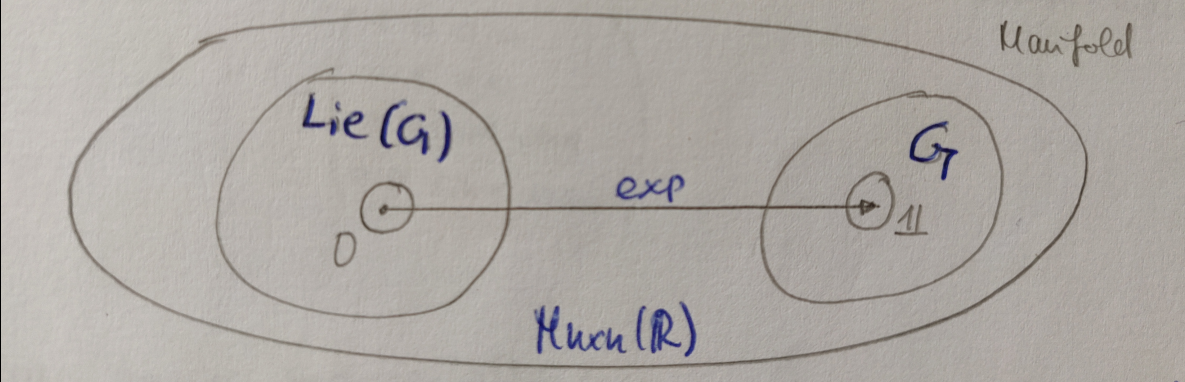
\includegraphics[width=0.7\linewidth]{gfx/Liegroups}
	\caption{\itshape Lie groups relation.}
	\label{fig:liegroups}
\end{figure}
$\Rightarrow exp(a)=g, a\in Lie(G), g\in G$ maps a small neighbourhood/patch of Lie(G) near $O$ to a small patch of $G$ near $\mathcal{I}$. If $a,b \in Lie(G)$, then 
$\exp([a,b])\in G$.
\begin{mybox}{Representation of a Lie-algebra}	
	\begin{equation}
		Lie(G) \stackrel{R}{\rightarrow} M(n), \quad a\mapsto R(a),
	\end{equation}
	with
	\begin{equation}
		R(0)=0, R([a,b])=R(a)R(b) -R(b)R(a) = [R(a),R(b)].
	\end{equation}
	Crucial:\\
	Given some representation $R$ of Lie-algebra Lie(G), we can always construct an associated representation of G (we call it also R) such that
	\begin{equation}
		R(A) = exp(R(a)) \quad if\quad A=\exp(a).
	\end{equation}
	Thus by having a representation of an element of Lie(G) 
	\begin{equation}
		w \, \Rightarrow \, w^{\nu} _{\mu}= -i \half \Omega_{\rho \sigma} (J^{\rho \sigma} )^{\nu}_{\mu} 
	\end{equation}
	we find a representation for an element of G
	\begin{equation}
		\Lambda^{\nu}_{\mu} =\left[\exp(-i \half \Omega_{\rho \sigma} (M^{\rho \sigma} ))\right]^{\mu}_{\nu}.
	\end{equation}
\end{mybox}
Consider $(J^{\rho \sigma})^{\nu}_{\mu}$ as the \emph{canonical basis} of so(1,3), thus these are the antisymmetric generators of SO(1,3). For $\Lambda \in SO(1,3)$ we find a $\tilde{\omega}$ such that we have a representation
\begin{align}
	\Lambda &= e^{\tilde{\omega}} \rightarrow \; \Lambda^{\;\nu}_{\mu} = \delta^{\nu}_{\mu} + \omega^{\nu}_{\mu} \\
	\omega^{\nu}_{\mu} &= -i \half \Omega_{\rho \sigma} (J^{\rho \sigma})^{\nu}_{\mu}.
\end{align}

\subsection{The Dirac spinor representation}
\begin{mybox}{Representation connected to spin }
	Spin $\half$ particles are described by fields in the \emph{spinor representation}.
\end{mybox}
\marginpar{Dirac algebra is a complexification of the real spacetime algebra  $Cliff(1,3,\mR): Cliff(1,3\mathbb{C}) = Cliff(1,3,\mR) \otimes \mathbb{C}$.}
\begin{mybox}{Dirac/Clifford algebra and spinor representation}
	
Every representation of Cliff(1,3) induces a representation of so(1,3). To find the spinor representation of so(1,3) we start from the Clifford algebra Cliff(1,3) defined as the algebra spanned by $n \times n$-matrices $(\gamma^{\mu})^A_B, \mu=0,1,2,3$ and $A,B=1,\dots,n$ such that the anti-commutator is
\begin{align}
	\{\gamma^{\mu}, \gamma^{\nu} \} & := 2 \eta^{\mu \nu} \mathcal{I}_{n\times n} \\
	\Rightarrow \gamma^{\mu} \gamma^{\nu} &= 
	\left\{ \begin{array}{lr}
		\eta^{\mu \nu} & if \mu =\nu \\
		- \gamma^{\nu} \gamma^{\mu} & if \mu\neq \nu
	\end{array}		\right\},
 \\
&(\gamma^0)^2=\mathcal{I},\quad (\gamma^i)^2 = - \mathbf{I}.
\end{align}
With the following object 
\begin{equation}
	(S^{\rho \sigma})^A_B := \frac{i}{4} [\gamma^{\rho},\gamma^{\sigma}]^A_B
\end{equation}
we find a basis of so(1,3), i.e.
\begin{equation}
	[S^{\rho \sigma}, S^{\tau \kappa} ] = -i \left[\eta^{\rho \kappa} S^{\sigma \tau} + \eta^{\sigma \tau} S^{\rho \kappa} - \eta^{\rho \tau} S^{\sigma \kappa} - \eta^{\sigma \kappa} S^{\rho \tau} \right].
\end{equation}
\end{mybox}

The Dirac algebra, thus the Cliff(1,3) algebra on $\mathbb{C}$, is then the standard environment the spinors of the Dirac equation live in, rather than the spacetime algebra.\\
Every representation of Cliff(1,3) induces a representation of Lie(SO(1,3)).\\
By defining $(S^{\rho \sigma})^A_B$ we have constructed a representation of Lie(SO(1,3)) and can from this representation infer a representation of SO(1,3) with $\Lambda \in SO(1,3)$:
\begin{equation}
	(\Lambda_{hald})^A_B = \left(e^{i \half \omega_{\mu \nu} S^{\mu \nu}} \right)^A_B.
\end{equation}
Or more precisely, we have constructed a basis and find a representation of this basis by choosing an explicit representation for the $\gamma^{\mu}$ matrices. From the basis we can construct the elements of $G$ by $\exp()$ and find therefore a representation of $G$.\\
The explicit representation of the Clifford algebra $Cliff(1,d-1)$ is given by the representation for it elements $\gamma^{\mu}$ by $n\times n$ matrices 
\begin{equation}
	(\gamma^{\mu})^A_B \quad \mathrm{with} \quad \mu\in \{0,1, \dots, d-1\}, A,B\in\{1,\dots, n \}.
\end{equation}
This will then also give a representation of $Lie(SO(1,d-1)) \Rightarrow$ The irreducible representations of $Cliff(1,d-1)$ are of dimension    $n=2^{d/2}$ if $d$ is even and $n=2^{\half (d-1)}$ if $d$ is odd.\\
Specialize to $d=4 \Rightarrow n=4 \Rightarrow$ Dirac representation (\emph{chiral})
\begin{align}
	\gamma^0 &= \begin{pmatrix}
		0 & \mathcal{I}_{2\times 2} \\
		\mathcal{I}_{2 \times 2} & 0 
	\end{pmatrix},
\quad 
\gamma^i=
\begin{pmatrix}
	0 & \sigma^i \\-\sigma^i &0
\end{pmatrix},
\\
\{\sigma^i, \sigma^j\} &=2 \delta^{ij}, \qquad \gamma^5=
\begin{pmatrix}
	-\mathcal{I}_{2\times 2} &0 \\
	0& \mathcal{I}_{2 \times 2}
\end{pmatrix}
\end{align}

\begin{mybox}{Dirac spinor representation}
	The complex vector space on which $(\gamma^{\mu})^A_B$ acts is called the space of Dirac spinors. A Dirac spinor is a set of field $\psi^A(x), A\in \{1,2,3,4\}$ transforming as
	\begin{equation}
		(\psi)^A(x) \mapsto [S(\Lambda)]^A_B (\psi)^B (\Lambda^{-1} x') = [S(\Lambda)]^A_B (\psi)^B(x) 
	\end{equation}
	with $[S(\Lambda)]^A_B = \left[\exp(-i \half \omega_{\rho \sigma} S^{\rho \sigma} )\right]^A_B$.\\
	$\Rightarrow$ A Dirac spinor field $(\psi)^A(x)$, with A,B \emph{spinor indices}, behaves \emph{like} spin $\half$-field, because
	\begin{equation}
		\Lambda(2 \pi) = \exp(i \half \omega_{\mu \nu} S^{\mu \nu} ) = - \mathcal{I}: (\psi)^A \mapsto -(\psi)^A.
	\end{equation}
\end{mybox}
The transformation of a Dirac spinor forms a representation of
\begin{equation}
	Spin(1,3) \cong \underbrace{SL(2, \mathbb{C})}_{\{M_{2 \times} (\mathbb{C}) \, and \, detM=1 \} }
\end{equation}
and not of $SO(1,3)$. Furthermore we know, that $Spin(1,3)$is the  \emph{double cover} of $SO(1,3)$.\\
This is equivalent to the fact that the $j=1/2$ spinor representation of the algebra of spatial rotations Lie(SO(3)) does not furnish a representation of the Lie group SO(3) but only of its double cover SU(2).\\
\begin{figure}[h]
	\centering
	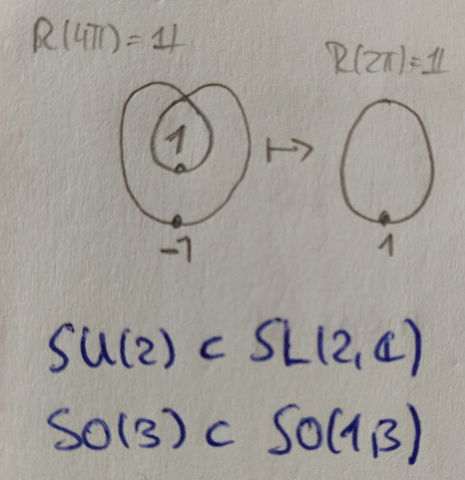
\includegraphics[width=0.7\linewidth]{gfx/doublecoverDiracSpinor}
	\caption{\itshape Double cover of the group, need to rotate by $4\pi$ to get back to the origin.}
	\label{fig:doublecoverdiracspinor}
\end{figure}

$\Rightarrow \psi_L, \psi_R$ transform under the irreducible representation of SO(1,3), $\psi=(\psi_L, \psi_R)^T$ only transforms under the reducible representation of Spin(1,3).




\subsection{The Dirac action}

We now have a new field, the Dirac spinor, and want to construct a covariant action for it.\\
Define the \emph{conjugate spinor}
 $\psi^{\dagger} := (\psi^*)^T= \left((\psi^1)^*, (\psi^2)^*, (\psi^3)^*, (\psi^4)^* \right)$. In the Dirac representation it is satisfied, that
 \begin{equation}
 	(\gamma^0)^{\dagger} = \gamma^0, \, (\gamma^i)^{\dagger} = - \gamma^i \; \Rightarrow \; (\gamma^{\mu})^{\dagger} = \gamma^0 \gamma^{\mu} \gamma^0
 \end{equation}
 and therefore we find
 \begin{equation}
 	\gamma^0 S[\Lambda]^{\dagger} \gamma^0 = S[\Lambda]^{-1}.
 \end{equation}
 To find the Lorentz-scalar for this theory, we define the \emph{Dirac conjugate spinor}
 \begin{equation}
 	\bar{\psi} = \psi^{\dagger} \gamma^0 \, \Rightarrow \bar{\psi} (x) \psi(x) 
 \end{equation}
 is a Lorentz scalar! Furthermore it holds, that $\bar{\psi} \gamma^{\mu} \psi$ is a Lorentz vector with 
 \begin{equation}
 	\bar{\psi} (x) \gamma^{\mu} \psi(x) \rightarrow \bar{\psi}(\Lambda^{-1} x') S^{-1}(\Lambda) \gamma^{\mu} S(\Lambda) \psi(\Lambda^{-1} x' )
 \end{equation}
 and thus
 \begin{equation}
 	S^{-1} (\Lambda) \gamma^{\mu} S(\Lambda) = \Lambda^{\mu}_{\nu} \gamma^{\nu}.
 \end{equation}
 \marginpar{Only a first order $\mL$, we had second order $\mL$ for scalar fields.}
 \begin{mybox}{Dirac field equations}

With those bilinears of the Dirac field $\bar{\psi} \gamma^{\mu} \psi, \bar{\psi} \psi$, each of which transforms covariantly under the Lorentz group, we find the 
\emph{Dirac action}
\begin{equation}
	S = \int \md^4 x \, \bar{\psi}(x) \left[i \gamma^{\mu} \partial_{\mu} - m\right] \psi(x)
\end{equation}
with $i$ needed for $S$ to be real and $|m|$ the mass of the Dirac spinor particle.\\
We find the \emph{Dirac equation}
\begin{align}
	\left(i \gamma^{\mu} \partial_{\mu} - m\right) \psi(x) &= 0\\
	\left(-i \partial_{\mu} \bar{\psi} \gamma^{\mu} - m \bar{\psi} \right)(x) &= 0.
\end{align}
If $\psi$ solves the Dirac equation, then $\psi$ solves the Klein-Gordon-equation ("Dirac eq. = $\sqrt{KG \, eq.}$").
 \end{mybox}

\subsection{Chirality and Weyl spinors}
\begin{mybox}{Weyl spinors}
	The Dirac spinor representation  of $Cliff(1,3)$ is not irreducible as a representation of $Spin(1,3)$, as the subspaces 
\begin{equation}
	\psi_- = (\psi_1,\psi_2,0,0)^T \quad \psi_+ = (0,0,\psi_3,\psi_4)^T
\end{equation}
transform \emph{seperately} under Lorentz transformations. The Weyl spinors $u_-$ $u_+$ form irreducible representations of $Spin(1,3): u_-=(\psi_1,\psi_2)^T, \quad u_+=(\psi_3,\psi_4)^T$.\\
\end{mybox}
A Dirac field can be projected onto its left-handed chirality and right-handed chirality components by
\begin{equation}
	\mathbb{P}_{\pm} := \half (\mathcal{I}\pm \gamma^5), \, \gamma^5 = i \gamma^0 \gamma^1 \gamma^2 \gamma^3 \quad\Rightarrow \; \psi_{\pm} = \mathbb{P}_{\pm} \psi.
\end{equation}
\marginpar{$\sigma^{\mu} = (\mathcal{I}_2, \sigma^i),\quad \bar{\sigma}^{\mu} = (\mathcal{I}_2 , - \sigma^i)$.}
In the context of these subspaces the Dirac action reads
\begin{equation}
	S = \int \md^4 x \left[u^{\dagger}_+ i \sigma^{\mu} \partial_{\mu} u_+ + u^{\dagger}_- i \bar{\sigma}^{\mu} \partial_{\mu} u_- -m(u^{\dagger}_+ u_-+ u^{\dagger}_- u_+) \right].
\end{equation}
\begin{mybox}{Weyl equations}
	If $m=0$, $u_+$ and $u_-$ decouple and describe independent degrees of freedom subject to the \emph{Weyl equations}:
	\begin{equation}
		i \sigma^{\mu} \partial_{\mu} u_+ (x) = 0, \quad i\bar{\sigma}^{\mu} \partial_{\mu} u_-(x)=0.
	\end{equation}
\end{mybox}
With the definition of the \emph{helicity} (=Chirality for $m=0$) 
\begin{equation}
	\hat{h} = \half \hat{\vec{p}} \cdot \vec{\sigma} = \half \begin{pmatrix}
	\hat{\vec{p}} \cdot \vec{\sigma } &0 \\
	0 & \hat{\vec{p}} \cdot \vec{\sigma}
	\end{pmatrix}.
\end{equation}
We find for $u_{\pm}(x) = u_{\pm}(p) e^{-i p\cdot x}$ 
\begin{equation}
	h u_{\pm} (p) = \pm \half u_{\pm} (p) \left\{	\begin{array}{lr}
	\Rightarrow u_+ & \mathrm{right-handed \, spinor} \\
	\Rightarrow u_- & \mathrm{left-handed \, spinor}
	\end{array}			\right\}.
\end{equation}




\subsection{Classical plane wave solutions}
There generally exist two solutions to the Dirac equation
\begin{align}
	\psi(x) &= u(\vec{p}) e^{- i p \cdot x}, \; u(\vec{p})= \begin{pmatrix}
		\sqrt{p \cdot \sigma} \xi \\
		\sqrt{p \cdot \bar{\sigma}} \xi 
	\end{pmatrix} 
\quad \mathrm{positive \, energy \, solution}\\
\psi(x) &= v(\vec{p}) e^{i p\cdot x}, \; v(\vec{p}) = \begin{pmatrix}
	\sqrt{p\cdot \sigma} \xi \\
	- \sqrt(p\cdot \bar{\sigma}) \xi
\end{pmatrix}
\quad 
\mathrm{negative\, energy\, solution}
\end{align}
with $\xi$ being a 2-component Weyl spinor.

\begin{mybox}{Completeness relation for four-spinors}
	\begin{align}
		\sum_s  u_s(\vec{p}) \bar{u}_s(\vec{p}) &= \gamma \cdot p+m\\
		\sum_s v_s(\vec{p}) \bar{v}_s(\vec{p}) &= \gamma \cdot p -m 
	\end{align}
\end{mybox}
with other relations being
\begin{align*}
	\bar{u}_s(\vec{p}) u_{s'}(\vec{p}) &= 2 m \delta_{s s'}, \quad u^{\dagger}_s(\vec{p})u_{s' }(\vec{p}) = 2 p^0 \delta_{s s'}, \\
	\bar{v}_s(\vec{p})v_{s'}(\vec{p}) &=-2 m \delta_{s s'},\quad v^{\dagger}_s(\vec{p}) v_{s'}(\vec{p}) = 2p^0 \delta_{s s'}\\
	\bar{u}_s(\vec{p}) v_{s'}(\vec{p}) &=0.
\end{align*}
With a basis of the 2-spinors given by $\xi_s: \left\{ \begin{array}{lr}
	\xi_{1/2} =(1,0)^T\\
	\xi_{-1 /2} = (0,1)^T
\end{array}	\right\} \Rightarrow u_s$ and $v_s$ with $s = \pm \half$ describe spinors with spin $\pm \half$ in direction $x_3$.

\subsection{Quantization of the Dirac field}
\begin{mybox}{Quantization procedure for spin $\half$ fields}
	Quantizing by imposing commutator relations is not possible, because the b-mode excitations would be negative norm states or equally because of unboundedness of the energy spectrum from below, i.e. instability of the vacuum.\\
	The correct procedure for quantization of spin-$\half$ fields is to impose the canonical anti-commutation relations:
	\begin{align}
		\{\psi^A(\vec{x}), \psi^{\dagger}_B(\vec{x}') \} &= \delta^A_B \delta^{(3)}_D(\vec{x}-\vec{x}')\\
		\{\psi^A(\vec{x}), \psi^B(\vec{x}') \} &=0=\{\psi^{\dagger}_A(\vec{x}), \psi^{\dagger}_B(\vec{x}) \}.
	\end{align}
This induces the mode relations
\begin{align}
	\{a_r(\vec{p}), a^{\dagger}_s(\vec{q}) \} &= (2 \pi)^3 \delta_{rs} \delta^{(3)}_D(\vec{p}-\vec{q}) \\
	\{b_r(\vec{p}), b^{\dagger}_s(\vec{q}) \} &= (2\pi)^3 \delta_{rs} \delta^{(3)}_D(\vec{p}-\vec{q}) \\
	\{a_r(\vec{p},b^{\dagger}_s(\vec{q})) \} &=0.
\end{align}
\end{mybox}
It follows that the Hamiltonian is given by
\begin{equation}
	H=\int \pmeasure E_p \sum_s \left[a^{\dagger}_s(\vec{p})a_s(\vec{p} )+v^{\dagger}_s(\vec{p}) b_s(\vec{p}) -(2 \pi)^3 \delta^{(3)}(\vec{0}) \right]
\end{equation}
with 
\begin{align}
	{H,a_s(\vec{p})} &= - E_p a_s(\vec{p}),\quad [H,a^{\dagger}_s(\vec{p})] =E_p a^{\dagger}_s(\vec{p}) \\
	[H,b_s(\vec{p})] &= - E_p b_s(\vec{p}), \quad [H, b^{\dagger}_s(\vec{p})] = E_p b^{\dagger}_s(\vec{p}).
\end{align}
$a^{\dagger}_s(\vec{p})$ creates a \emph{fermion} of momentum $\vec{p}$ and spin $s$, and $b^{\dagger}_s(\vec{q})$ creates an \emph{anti fermion} of momentum $\vec{q}$ and spin $r$.\\
The general field $\psi(x)$ is now seen to be a weighted summation over all possible spins and momenta for creating fermions and anti fermions 
\begin{equation}
		\psi(x) = \sum_s \int \pmeasure \frac{1}{\sqrt{2E_p}} \left[a_s(\vec{p})u_s(\vec{p} e^{-ip\cdot x} + b^{\dagger}_s(\vec{p}))v_s(\vec{p}) e^{i p\cdot x}  \right].
\end{equation}
Its conjugate field $\bar{\psi}$ is a weighted summation over all possible spins and momenta for annihilating fermions and anti fermions $\bar{\psi}=\psi^{\dagger} \gamma^0$
\begin{equation}
	\psi^{\dagger} (x) = \sum_s \int \pmeasure \frac{1}{\sqrt{2 E_p}} \left[b_s(\vec{p})v^{\dagger}_s(\vec{p})e^{-i p\cdot x} + a^{\dagger}_s(\vec{p}) u^{\dagger}_s(\vec{p}) e^{i p\cdot x} \right].
\end{equation}
We furthermore know
\begin{align}
	\Pi &= \frac{\partial \mL_D}{\partial(\partial_0 \psi)} = i \psi^{\dagger} \quad \mathrm{canonically \, conjugated\, momentum}\\
	\mathcal{H}_D &= \bar{\psi} \left[- i \vec{\gamma} \cdot \vec{\nabla} +m\right] \psi \quad \mathrm{Hamiltonian\, density}.
\end{align}
Note further, that the divergent vacuum energy has \emph{opposite} sign compared to a scalar theory.\\
\\
\\
From the vacuum 
\begin{equation}
	a_s(\vec{p})\ket{0} = 0 = b_s(\vec{p}) \ket{0} \quad \forall \vec{p}
\end{equation}
\marginpar{a-modes$\equiv$ "particle sector".}
we can now construct the Fock space of a- and b-mode excitations:
\begin{enumerate}
	\item The state $\ket{\vec{p},s} :=\sqrt{2E_p}a^{\dagger}_s(\vec{p})\ket{0}$ is a 1-particle state with momentum $ \vec{p}$, energy $E_p=\sqrt{\vec{p}^2+m^2}$ and spin $s=\half,-\half$ in $x_3$-direction.
	\begin{align}
		\braket{\vec{p},s}{\vec{q},r} = 2 E_p (2 \pi)^3 \delta^{(3)}_D(\vec{p}-\vec{q}) \delta^{rs} \\
		\ket{\vec{p}_1,s_1;\dots;\vec{p}_N,s_N} &= \prod_{i=1}^{N} \sqrt{2 E_{p_i}} a^{\dagger}_{s_1} (\vec{p}_1) \dots a^{\dagger}_{s_N} (\vec{p}_N) \ket{0}.
	\end{align}
\item By the anti-commutation relations we state the theorems:
\begin{statements}
	The wavefunction of $N$-particle states of spin $\half$ particles is anti-symmetric under particle exchange.\\
	$\Rightarrow$ spin-$\half$ particle obey \emph{Fermi-Dirac statistics}, i.e. they are \emph{fermions}.\\
	$\Rightarrow$ \emph{Pauli-exclusion principle}:\\
	No two fermionic states of exactly the same quantum numbers are possible.
\end{statements}
\item \begin{mybox}{Spin-Statistics Theorem}
	This can be cast more generally into the \emph{Spin-Statistics-Theorem:}\\
	$\rightarrow$ Particles of half-integer spin are \emph{fermions} and \\
	$\rightarrow$ particles of integer spin are \emph{bosons}.
\end{mybox}
\item The Dirac Lagrangian satisfies a global $U(1)$ symmetry with $j^{\mu} =\bar{\psi} \gamma^{\mu} \psi$\\
\begin{align}
	Q&= \int \pmeasure \sum_s \left[a^{\dagger}_s(\vec{p})a_s(\vec{p})  -b^{\dagger}_s(\vec{p}) b_s(\vec{p}) \right]\\
	\Rightarrow & \left\{		\begin{array}{lr}
		Qa^{\dagger}_s(\vec{p}) \ket{0} &=+a^{\dagger}_s(\vec{p}) \ket{0} \, \leftrightarrow\, \mathrm{fermion\, of \, spin} s, \mathrm{momentum} \vec{p} \\
		Q b^{\dagger}_s(\vec{p}) \ket{0} &=-b^{\dagger}_s(\vec{p}) \ket{0} \, \leftrightarrow \, \mathrm{anti \, fermion \, of \, spin} s, \mathrm{momentum} \vec{p}.
	\end{array}		\right\}
\end{align}

\end{enumerate}

\subsection{Propagator}
In the Heisenberg picture we find the propagator to be
\begin{align}
	S^A_{\,B}(x-y) &:= \{\psi^A(x), \bar{\psi}_B(y) \} \\
	\Rightarrow S(x-y) &= (i \gamma^{\mu} \partial_{x^{\mu}}+m) \left[D^{(0)}(x-y) - D^{(0)}(y-x) \right]\\
	&= \int \pmeasure \frac{1}{2 E_p} \left[(\gamma_{\nu} p^{\nu} +m_0) e^{-ip(x-y)} + (\gamma_{\nu}p^{\nu} -m_0) e^{-ip(y-x)}  \right].
\end{align}
With this we have $S(x-y)=0$ for $(x-y)^2<0$ outside the lightcone; this in turn guarantees $[O_1(x),O_2(y)]=9$ for $(x-y)^2<0$, because all observables are bilinear in fermions, these still commute outside the lightcone. This establishes causality of the Dirac theory.\\
\\ The propagator satisfies $(i \slashed{\partial}_x -m)S(x-y)=0$ (because $p^2=m^2$). This follows from ($\slashed{\partial}^2_x + m^2) D^{(0)}(x-y) =0$.
\\
\\ The time-ordering symbol in the fermionic theory is defined by an \emph{additional minus sign}
\begin{equation}
	\hat{T}[\psi(x),\bar{\psi}(y)] = \left\{\begin{array}{lr}
	\psi(x)\bar{\psi}(y) & \mathrm{if} \, x^0 \geq y^0\\
	-\bar{\psi}(y) \psi(x) & \mathrm{if} \, y^0 > y^0.
	\end{array}		\right\}
\end{equation}
\begin{mybox}{Feynman propagator in fermionic theory}
	The Feynman propagator is
	\begin{equation}
	S_F(x-y) = \expval{\hat{T}[\psi(x),\bar{\psi}(y)]}{0} = \int \frac{\md^4 p}{(2 \pi)^4} \frac{i (\gamma \cdot p +m_0)}{p^2-m^2_0 +i\epsilon} e^{-i p \cdot (x-y)}.
	\end{equation}
	The Feynman propagator is the Green's function of the Dirac operator 
	\begin{equation}
		(i \slashed{\partial} -m) S_F(x-y) = i \delta^{(4)}_D(x-y).
	\end{equation}
	For computations use
	\begin{align}
		/\slashed{p}-m) \frac{\slashed{p}+m}{p^2-m^2} &= \mathcal{I}, \\
		\frac{\slashed{p}+m}{p^2-m^2} &= \frac{\mathcal{I}}{\slashed{p} -m},
	\end{align}
these are matrices, \emph{beware}.
\end{mybox}





\subsection{Wick's theorem and Feynman diagrams}
\begin{mybox}{Fermionic time ordering}
	The time ordering of several fields picks up a minus sign whenever $2$ fermionic fields are exchanged, i.e. multiply by $(-1)$ for every adjacent permutation of two fields.
\end{mybox}
\begin{mybox}{Fermionic normal ordering}
	We define \emph{normal-ordered} products as expressions with all annihilation/creation operators to the right/left, \emph{but here each exchange of two operators induces a minus sign}, beware !
	\begin{align}
		\hat{T}[\psi(x),\bar{\psi}(y)] &= \normord{\psi(x) \bar{\psi}(y)} + \contraction{}{\psi(x)}{}{\bar{\psi}(y)} \psi(x) \bar{\psi}(y) \\
		\contraction{}{\psi(x)}{}{\bar{\psi}(y)} \psi(x) \bar{\psi}(y) &= \expval{\hat{T}[\psi(x) \bar{\psi}(y)]}{0} = S_F(x-y) \\
		\contraction{}{\psi(x)}{}{\psi(y)} \psi(x) \psi(y) &= 0 \quad = \contraction{}{\bar{\psi}(x)}{}{\bar{\psi}(y)}\bar{\psi}(x) \bar{\psi}(y).
	\end{align}
\end{mybox}
\begin{mybox}{Wick's theorem for fermions}
	\begin{equation}
	\hat{T}[\bar{\psi}_1 \bar{\psi}_2 \psi_3 \dots ] = \normord{\bar{\psi}_1 \bar{\psi}_2 \psi_3 \dots } + \normord{\mathrm{all\,contractions\,with\,signs}}.
	\end{equation}
	In particular
	\begin{equation}
		\expval{\hat{T}\left[\prod_i \psi(x_i) \prod_j \bar{\psi}(\bar{x}_j) \right]}{0} \neq 0
	\end{equation}
	only for equal numbers of $\psi$ and $\bar{\psi}$ fields. Physically this just reflects \emph{charge conservation}.
\end{mybox}
\begin{mybox}{Feynman-diagrams for fermions} 
	To compute a $2n$-point function, we draw corresponding Feynman diagrams, but now
	\begin{enumerate}
		\item Label the points $x_i$ associated with $\psi(x_i)$ and $\bar{x}_j$ associated with $\bar{\psi}(\bar{x}_j)$ separately.
		\item Only connect $x_i$ and $\bar{x}_j$.
		\item Associate each directed line from $\bar{x}_j$ to $x_i$ with a propagator \begin{equation} 
		S_F(x_i-\bar{x}_j) = \feynmandiagram[horizontal=a to b]{a [label=$x_i$] -- [anti fermion] b [particle=$\bar{x}_j$] };
		\end{equation}
	\end{enumerate}
Always draw the arrow from $\bar{x}_j$ to $x_i$ in order to account for the correct sin in $S_F(x_i - \bar{x}_j)$.\\
\begin{statements}
The relative sign between the diagrams is equal to the numbers of crossing lines.
\end{statements}
\end{mybox}

\subsection{LSZ and Feynman rules}
In the presence of interactions we define asymptotic in-and out-fields satisfying the free Dirac equation with mass $m\neq m_0$, where $m_0$ is the mass of the Dirac action.\\
We then express the creation and annihilation modes by the in-and out-fields:
\begin{align}
	a_{in,s}(\vec{q}) &= \frac{1}{\sqrt{2 E_q} } \int \md^3 x \bar{u}_s(\vec{q}) e^{i q\cdot  x} \gamma^0 \psi_{in}(x) \\
	a^{\dagger}_{in,s}(\vec{q}) &= \frac{1}{\sqrt{2 E_q}} \int \md^3 x \bar{\psi}_{in} (x) \gamma^0 e^{ -i q \cdot x} u_s(\vec{q}) \\
	b_{in,s}(\vec{q}) &= \frac{1}{\sqrt{2 E:q}} \int \md^3 x \bar{\psi}_{in}(x) \gamma^0 e^{i q\cdot x} v_s(\vec{q}) \\
	b^{\dagger}_{in,s}(\vec{q}) &= \frac{1}{\sqrt{2 E_q}} \int \md^3 x \bar{v}_s(\vec{q}) e^{-i q\cdot x} \gamma^0 \psi_{in}(x).
\end{align}
\begin{mybox}{LSZ formula for fermions}
Consider incoming fermions $\ket{q,s,+}$ and anti fermions $\ket{q',s',-}$ and outgoing fermions $\bra{p,r,+}$ and anti fermions $\bra{q',r',-}$: Note that $n=\#$ fermions and $n'=\# anti-fermions$ as well as $m=$ \emph{fully renormalized} physical mass:
\begin{align}
	&\bra{\dots (p,r,+) \dots (p',r',-) \dots} S \ket{\dots (q,s,+) \dots (q',s',-) \dots }_{connected}\nonumber  \\
	&= \left(-i Z\right)^{- n \half } \left(i Z\right)^{- n' \half}  \int \md^4 x \dots \int \md^4 x'\dots \int \md^4 y \dots \int \md^4 y'  \nonumber\\
	&\exp(\left\{ -i \left(q\cdot x+q'\cdot x'-p \cdot y - p'\cdot y' + \dots \right)     \right\}) \nonumber \\
	&\bar{u}_r(\vec{p})  (i \gamma \cdot \partial_y -m) \dots \bar{v}_{s'} (\vec{q}')(i \gamma \cdot \partial_{x'} -m) \nonumber \\
	& \expval{\hat{T}\left[\dots \bar{\psi}(y') \dots \psi(y) \dots \bar{\psi}(x) \dots \psi(x') \dots \right]}{\Omega}\nonumber \\
	& (-i \gamma \cdot \stackrel{\leftarrow}{\partial}_x -m) u_s(\vec{q}) \dots (-i \gamma \cdot \stackrel{\leftarrow}{\partial}_y -m) v_{r'}(\vec{p} ').
\end{align}
\end{mybox}
\begin{mybox}{Feynman diagrams and S-matrix for fermions}
	Thus to compute the S-matrix we compute the Fourier transform of the amputated fully connected associated Feynman diagram, where for each external particle we include 
	\begin{enumerate}
		\item $u_s(\vec{q})$ for an incoming particle of spin $s$,
		\item $\bar{v}_{s'}(\vec{q}')$ for an incoming anti-particle of spin $-s'$,
		\item $\bar{u}_r(\vec{p})$ for an outgoing particle of spin $r$,
		\item $v_{r'}(\vec{p}')$ for an outgoing anti-particle of spin $-r'$.
	\end{enumerate}
\end{mybox}









\newpage 
\section{Quantizing Spin $1$-fields}
\subsection{Maxwell's equations (classical) }
The action for Maxwell's equation is 
\begin{equation}
	S = \int \md^4 x \left[-\frac{1}{4} F_{\mu \nu} F^{\mu \nu} - A_{\mu}j^{\mu} \right]
\end{equation}
with $F^{\mu \nu} = \partial^{\mu} A^{\nu}- \partial^{\nu} A^{\mu}, j^{\mu} = (\rho, \vec{j})^T, A^{\mu} = (\phi, \vec{A})^T$.\\
The \emph{inhomogeneous Maxwell equations} follow with
\begin{equation}
	\partial_{\mu} F^{\mu \nu} = j^{\nu}.
\end{equation}
Two of the Maxwell equations are given by the Bianchi identity 
\begin{equation}
	\partial_{\lambda} F_{\mu \nu} + \partial_{\mu} F_{\nu \lambda} + \partial_{\nu} F_{\lambda \mu } = 0 \; \Rightarrow \; \partial_{\mu} j^{\mu} = 0 
\end{equation}
follows ($S$ is gauge invariant if and only if this charge conservation holds).\\
$F^{\mu \nu}$ and thus $\vec{E}$ and $\vec{B}$ are invariant under a \emph{local gauge transformation}
\begin{equation}
	A^{\mu}(x) \rightarrow A^{\mu}(x) + \partial^{\mu} \alpha(x) 
\end{equation}
for any function $\alpha(x)$ with $\lim_{\vec{x}\rightarrow \infty} \alpha(x) =0$. Configurations related by gauge transformations are physically equivalent. Gauge symmetries merely denote a redundancy in the description of the system.
\begin{mybox}{Lorenz gauge}
	Pick $A^{\mu}$ such that 
	\begin{equation}
		\partial_{\mu} A^{\mu} =0,
	\end{equation}
	which still leaves us with the freedom of a residual gauge transformation
	\begin{equation}
		A^{\mu} \rightarrow A^{\mu} + \partial^{\mu} \phi \quad \mathrm{with} \quad \partial^2 \phi =0.
	\end{equation}
	$\Rightarrow$ In Lorentz gauge the equation of motions is
	\begin{equation}
		\partial^2 A^{\mu} = j^{\mu}.
	\end{equation}
	Lorenz gauge is implemented in the action by a Lagrange multiplier
	\begin{align}
		S&= \int \md^4 x \left[- \frac{1}{4} F_{\mu \nu} F^{\mu \nu} - \frac{\lambda}{2} (\partial_{\alpha} A^{\alpha})^2- A_{\beta}j^{\beta}\right]\\
	\stackrel{e.o.m.}{\Rightarrow} & 
	\left\{\begin{array}{lr}
		\partial^2 A^{\mu} - (1-\lambda) \partial^{\mu} (\partial \cdot A) = j^{\mu} \\
		\partial \cdot A = 0
	\end{array}
	\right\}
	\end{align}
This equation (Lorentz gauge) will be implemented at a specific point during quantization, not before.
\end{mybox}

\subsection{Canonical Quantization of the free field}
\begin{mybox}{Complications in quantization procedure}
	Quantizing a free ($j^{\mu}=0$) non-gauge fixed Lagrangian doesn't work, \emph{because $A^0$ is not a dynamical field} $\Rightarrow \Pi_{\mu}=F_{0\mu} \Rightarrow \Pi_0=0$. Instead quantization starts from the gauge fixed Lagrangian
	\begin{equation}
		\mL = - \frac{1}{4} F_{\mu \nu} F^{\mu \nu} - \frac{\lambda}{2} (\partial \cdot A)^2
	\end{equation}
	\begin{equation}
		\Rightarrow \Pi_{\mu} = \frac{\partial \mL}{\partial \dot{A}^{\mu}} = F_{\mu 0} \quad - \lambda \eta_{\mu 0} (\partial \cdot A).
	\end{equation}
\end{mybox}
With $\lambda=1$, this choice is called \emph{Feynman gauge}, the equation of motion of $\lambda$, namely $\partial \cdot A=0$, has now to be imposed \emph{by hand} as a constraint:
\begin{equation}
	\Rightarrow  \; \mL = -\frac{1}{4} F_{\mu \nu} F^{\mu \nu} = - \half \partial_{\mu}A_{\nu}\partial^{\mu} A^{\nu} \quad \mathrm{with} \quad \partial \cdot A =0.
\end{equation}
The equations of motion for $A^{\mu}$ are 
\begin{equation}
	\partial^2 A^{\mu} =0 \quad \mathrm{together\, with\, } \partial \cdot A=0.
\end{equation}
And the canonical momentum density is
\begin{equation}
	\Pi_{\mu} = - \dot{A}_{\mu}.
\end{equation}
\begin{mybox}{Canonical equal-time commutators for photons}
	Quantize by promoting $A_{\mu},\Pi_{\mu}$ to Heisenberg operator field with \emph{canonical equal-time commutators}
	\begin{align}
		\left[A^{\mu} (\vec{x},t) , \dot{A}^{\nu}(\vec{y},t)\right] &= - i \eta^{\mu \nu} \delta^{(3)}_D(\vec{x}-\vec{y}), \\
		\left[A^{\mu} (\vec{x},t), A^{\nu}(\vec{y},t)\right] &= 0= \left[\dot{A}^{\mu}(\vec{x},t), \dot{A}^{\nu}(\vec{y},t)\right],
	\end{align}
which imply the mode expansion for the photon field
\begin{equation}
	A^{\mu}(x) = \int \pmeasure \frac{1}{\sqrt{2 E_p}} \int_{\lambda=0}^{3} \epsilon^{\mu} (\vec{p},\lambda) \left[a_{\lambda}(\vec{p}) e^{-i p\cdot x} + a^{\dagger}_{\lambda} (\vec{p}) e^{ip\cdot x} \right],
\end{equation}
which solves $\partial^2 A^{\mu}=0$ for $p^2=0 \Rightarrow E_p = |\vec{p}|$ for photons and it implies $\Rightarrow p^{\mu}$\emph{ lightlike} !\\
The vectors $\epsilon^{\mu}(\vec{p},\lambda)$ are \emph{four linearly independent real polarization vectors}. We pick their normalization to be
\begin{equation}
	\epsilon(\vec{p},\lambda) \cdot \epsilon(\vec{p},\lambda') = \eta_{\lambda, \lambda'} = \delta_{\lambda,\lambda'}.
\end{equation}
\end{mybox}
We pick the four $\epsilon^{\mu}$ to be the following, let $n^{\mu}$ denote the times axis with $n^2 =1$: 
\marginpar{The basis of polarization vectors depends on the concrete momentum $p$ with $p^2=0$.}
\begin{enumerate}
	\item $\epsilon^{\mu}(\vec{p},0)=n^{\mu}$: timelike/scalar polarization vector,
	\item $\epsilon^{\mu} (\vec{p}, i), \; i=2,1$: transverse polarization vectors with $\epsilon(\vec{p},i)\cdot n =0=\epsilon(\vec{p},i) \cdot p$ \& $\epsilon(\vec{p},i) \cdot \epsilon(\vec{p},j) = - \delta_{ij}$,
	\item $\epsilon^{\mu}(\vec{p},3)$ longitudinal polarization vector with $\epsilon(\vec{p},3) = \frac{p-n (p\cdot n)}{p+n}$.
\end{enumerate}
\begin{mybox}{Photon ladder operator commutation relations}
	In this theory we find 
	\begin{align}
		\left[a_{\lambda}(\vec{p}), a^{\dagger}_{\lambda'} (\vec{p}')\right] &= - \eta_{\lambda, \lambda'} (2 \pi)^3 \delta^{(3)}_D(\vec{p}-\vec{p}') \\
		\left[a_{\lambda}(\vec{p}), a_{\lambda'}(\vec{p}') \right] &= 0 \quad = \left[a^{\dagger}_{\lambda} (\vec{p}), a^{\dagger}_{\lambda '} (\vec{p}') \right].
	\end{align}
\end{mybox}
\begin{mybox}{Fock space for photons}
As usual, from these the Hamiltonian and construction of the Fock space follows straightforwardly:
\begin{align}
	H &= \half \int \md^3 x \left[- \dot{A}^{\mu} \dot{A}_{\mu} + \partial_i A_{\mu} \partial^i A^{\mu} \right] \nonumber \\
	 &= \int  \pmeasure |\vec{p}| \left[\sum a^{\dagger}_i(\vec{p}) a_i(\vec{p}) -a^{\dagger}_0(\vec{p}) a_0(\vec{p})\right]
\end{align}
where the latter equality follows \emph{after dropping the vacuum energy}. The Fock space follows then with
\begin{align}
[H,a^{\dagger}_{\lambda} (\vec{p})] & = + |\vec{p}| a^{\dagger}_{\lambda}(\vec{p}) \\
	[H,a_{\lambda}(\vec{p})] &=-|\vec{p}| a_{\lambda}(\vec{p}) \\
	\Rightarrow \; a_{\lambda}(\vec{p}) \ket{0} &=0.
\end{align}
The \emph{1-particle} state is here defined via
\begin{equation}
	\ket{\vec{p},\lambda} := \sqrt{2 E_p} a^{\dagger}_{\lambda}(\vec{p}) \ket{0}
\end{equation}
as the states of momentum $\vec{p}$ and polarization $\lambda$. The corresponding photons are called \emph{photons}.
\end{mybox}
\begin{mybox}{Ghosts and complications with unitarity}
	Due to the minus sign in the commutator we find time-like polarization ($\lambda=0$) states to have a negative norm
	\begin{equation*}
		\braket{\vec{p},0}{\vec{q},0} \propto \expval{[a(\vec{p},0), a^{\dagger}(\vec{q},0)]}{0} = - (2 \pi)^3 \delta^{(3)}_D(\vec{p}-\vec{q}).
	\end{equation*}
Such negative norm states are called \emph{ghosts} and spoil unitarity.\\
$\Rightarrow$ The problems are solved if we implement now the Lorenz gauge. It will remove timelike, negative norm states and furthermore \emph{cut the physical polarizations down to two}.
\end{mybox}


\subsection{Gupta-Bleuler quantization}
The \emph{Gupta-Bleuler} formalism directly implements the Lorenz gauge condition on the physical states of our Hilbert space. We define a physical Hilbert space by the \emph{Gupta-Bleuler condition}
\begin{equation}
	\phi \in \mathcal{H}_{physical} \quad \leftrightarrow \quad \partial^{\mu} A^+_{\mu} \ket{\phi} = 0
\end{equation}
with $A_{\mu}(x) = A^+_{\mu}(x) +A^-_{\mu}(x)$.\\
\\
For a 1-photon state of general polarization $\zeta^{\mu}$ with
\begin{align}
	\zeta^{\mu} &= \sum_{\lambda,\lambda'} \alpha_{\lambda} \eta_{\lambda, \lambda'} \epsilon^{\mu}(\vec{p},\lambda) \\
	\ket{\vec{p},\zeta} &:= \sqrt{2 |\vec{p}|} \sum_{\lambda} \alpha_{\lambda} a^{\dagger}_{\lambda} (\vec{p}) \ket{0}.
\end{align}
\begin{mybox}{Phyical states and polarizations}
This condition equivalently reads
\begin{equation}
	\ket{\vec{p},\zeta} \in \mathcal{H}_{physical} \quad \leftrightarrow\quad p^{\mu} \zeta_{\mu} = 0.
\end{equation}
One can furthermore decompose the photon state like
\begin{equation}
	\ket{\vec{p},\zeta} = \ket{\vec{p},\zeta_T} + \ket{\vec{p},\zeta_s}
\end{equation}
where 
\begin{enumerate}
	\item $\ket{\vec{p},\zeta_T}$ describes 2 transverse degrees of freedom of positive norm, $\norm{\ket{\vec{p},\zeta_T}} >0$.
	\item $\ket{\vec{p},\zeta_s}$ describes 1 combined timelike and longitudinal degree of freedom of zero no norm, $\norm{\ket{\vec{p},\zeta_s}} =0$.
	\item $\Rightarrow$ One find this theorem to be true:
	\begin{statements}
		The state $\ket{\vec{p},\zeta_s}$ decouples from all physical processes
	\end{statements}
\end{enumerate}
\end{mybox}
Such a zero-norm state that decouples from all physical processes is called \emph{spurious}:
\begin{equation}
	\expval{O}{\vec{p},\zeta_s} = 0 \quad \forall \mathrm{observables \, in \, a \, free \, theory.}
	\end{equation}
Generally, as long as the interactions respect gauge invariance, a spurious state $\ket{\vec{p},\zeta_s}$ decouples from the S-matrix as an external (in or out) state $\Rightarrow$ Only the 2 transverse polarizations are physically relevant as external state.
\\
\\
\begin{statements}
	Massless vector fields have two physical degrees of freedom.
\end{statements}



\subsection{Coupling vector fields to matter}

\marginpar{Note that massless vector fields have two physical degrees of freedom.}
\begin{mybox}{On connection of mass and gauge invariance}
	
Lorentz invariance requires invariance of the action under gauge transformations, because any Lorentz vector field describing 2 polarization  states transforms under a Lorentz transformation 
\begin{equation}
	A^{\mu}(x) \rightarrow \Lambda^{\mu}_{\nu} A^{\nu} (\Lambda^{-1} x') \quad + \partial^{\mu} \epsilon (x,\Lambda)
\end{equation}
Furthermore, $\mL = -\frac{1}{4} F_{\mu \nu} F^{\mu \nu}$ is the \emph{unique} Lorentz invariant and gauge invariant Lagrangian for a massless free vector field.
\begin{statements}
	The mass term for a massive vector boson explicitly breaks gauge invariance. Massless vector field theories must be gauge theories.
\end{statements}
\end{mybox}
\begin{mybox}{Coupling the massless vector theory to matter}
	We would like to couple a massless vector field $A^{\mu}(x)$ to a matter sector, e.g. a Dirac fermion or a. scalar field (denoted with $\phi$ here). We can construct such a coupled action
	\begin{equation}
		S = S^0_A[A] \quad +S_{int} [A,\phi] \quad + S^{rest}_{matter} [\phi].
	\end{equation}
$\rightarrow$	If $S_{int}[A,\phi]$ is chosen such, that the successful decoupling of negative norm states and zero norm states in the free vector theory is not spoiled by the interaction. This constraint is formulated by the \emph{Ward identity} for QED
\begin{equation}
	k_{\mu} M^{\mu} =0
\end{equation}
\end{mybox}
Such that external photons of polarization $\zeta_{\mu} (k) = k_{\mu}$ decouple from the interactions. This uncoupling is equivalent to the statement, that the vector theory must couple to a conserved current 
\begin{equation}
	- \frac{\delta S_{int} [A,\phi]}{\delta A^{\mu}} = - j^{\mu},
\end{equation}
with $j^{\mu}$ for $U(1)$ global symmetry.\\
If $S^0_A[A]$ is \emph{invariant} under the gauge symmetry
\begin{equation}
	A_{\mu}(x) \rightarrow A_{\mu} (x) \quad + \partial_{\mu} \alpha(x)
\end{equation}
then the coupling to a conserved $U(1)$ current is equivalent to the statement that the full action $S$ is invariant under the combined gauge transformation, and therefore \emph{equivalent} to the Ward identity 
\begin{equation}
	\phi(x) \rightarrow \phi(x) - e \alpha(x) \delta\phi(x) \; \& \; A_{\mu}(x) \rightarrow A_{\mu}(x) + \partial_{\mu} \alpha(x).
\end{equation}
The process of promoting the global continuous $U(1)$ symmetry to a combined gauge symmetry is called \emph{gauging}.

\subsubsection{Coupling to Dirac fermions}
We now want to apply this gauge process to the free Dirac fermion action
\begin{equation}
	S^{rest}_{matter} = \int \md^4 x \; \bar{\psi} (i \gamma \cdot \partial - m_0 ) \psi.
\end{equation}
\begin{mybox}{Gauging the free Dirac theory $\Rightarrow$ Quantum Electrodynamics}
	The Dirac Lagrangian has a global $U(1)$ symmetry with an associated conserved current. We find the gauge invariant QED Lagrangian if we gauge the Dirac theory by promoting the global $U(1)$ symmetry to a local one:
	\begin{equation}
		\psi(x) \rightarrow e^{-i e \alpha(x)} \psi(x), \quad j^{\mu} = e \bar{\psi} \gamma^{\mu} \psi.
	\end{equation}
	The interaction term is then \emph{invariant under the combined gauge transformation} ! Thus the decoupling of unphysical photon states is satisfied:
	\begin{equation}
		\psi(x) \rightarrow e^{-i e \alpha(x) } \psi(x), \quad A_{\mu} \rightarrow A_{\mu} + \partial_{\mu} \alpha(x),
	\end{equation}
	which can be written in terms of the \emph{covariant derivative}
	\begin{equation}
		D_{\mu} := \partial_{\mu} + i e A_{\mu} \quad \Rightarrow \quad D_{\mu} \psi(x) \rightarrow e^{-i \alpha(x)} D_{\mu} \psi(x).
	\end{equation}
	Thus, the Lagrangian is \emph{manifestly gauge-invariant} off-shell
	\begin{equation}
		\mL_{QED} = \underbrace{- \frac{1}{4} F_{\mu \nu} F^{\mu \nu} }_{=-\half \partial_{\mu} A_{\nu} \partial^{\mu} A^{\nu}} + \bar{\psi} (i \gamma^{\mu} D_{\mu} -m_0) \psi.
	\end{equation}
	In other words, the equations of motion of QED read
	\begin{align}
		\partial_{\nu} F^{\nu \mu} &= e \bar{\psi} \gamma^{\mu} \psi \\
		\stackrel{\partial \cdot A=0}{\Leftrightarrow} \partial^2 A^{\mu} &= e \bar{\psi} \gamma^{\mu} \psi.
	\end{align}
	
\end{mybox}
In QED we set $e=-|e|$ equal to the \emph{elementary charge of one electron}, such that 
\begin{equation}
	\left\{	
	\begin{array}{lr}
	Qa^{\dagger}_s(\vec{p}) \ket{0} =- |e| a^{\dagger}_s(\vec{p}) \ket{0} \quad \mathrm{for \, an \, electron} \\
	Q b^{\dagger}_s(\vec{p}) \ket{0} = + |e| b^{\dagger}_s(\vec{p} ) \ket{0} \quad \mathrm{for \, a \, positron}
	\end{array}
	\right\},
\end{equation}
where $Q=e \int \md^3 x \bar{\psi} \gamma^0 \psi = e \int \md^3 x j^0$.
\\
\\
\subsubsection{A subtle note on gauge symmetry}
There is a big difference between the interpretation of a global symmetry and a gauge symmetry. The former takes you from one physical state to another with the same properties and results in a conserved current through Noeher's theorem. The latter is redundancy in our description of the system. Yet here it seems like gauge symmetry leads to a conservation law, namely the \emph{conservation of electric charge}. This is because among the infinite number of gauge symmetries parametrized by a function $\alpha(x)$, there is also a \emph{single} global symmetry: that with $\alpha(x) =$ constant. This is a \emph{true} symmetry of the system, meaning that it takes us to another physical state.\\
\\
Note that coupling to complex scalars with $U(1)$ symmetry is possible by the \emph{minimal coupling prescription} $\partial_{\mu} \rightarrow D_{\mu}$. By this, the gauge invariance of the combined matter and gauge sector is ensured.



\subsection{Feynman rules for QED}
We will now study interactions of QED, whose Lagrangian is given by
\begin{equation}
	\mL_{QED} = -\frac{1}{4} F_{\mu \nu} F^{\mu \nu} - \underbrace{\frac{\lambda}{2} (\partial \cdot A)^2}_{=0 \, in \, Feynman \, gauge} + \bar{\psi} (i \gamma\cdot \partial -m_0) \psi - e A_{\mu} \bar{\psi} \gamma^{\mu} \psi.
\end{equation}
This theory describes \emph{the coupling of the Maxwell $U(1)$ gauge potential to electro-magnetically charged spin $\frac{1}{2}$ particles of free mass $m_0$.}
\begin{mybox}{Feynman propagator for the photon/gauge field}
	The Feynman propagator for the gauge field in Feynman gauge is
\begin{align}
	\expval{\hat{T}\{A^{\mu} (x) A^{\nu}(y) \}}{0} &= - \eta^{\mu \nu} D^{(0)}_F(x-y) |_{m^2_0=0}\nonumber \\
	& = \int \frac{\md^4 p}{(2 \pi)^4} \frac{- i \eta^{\mu \nu}}{p^2 +i \epsilon} e^{-i p\cdot (x-y)}.
\end{align}
\end{mybox}
		\todo{try to get feynman diagrams correctly positioned as a wedge}
\vspace{1cm}
		The Feynman rules for QED are the following:\\
	To compute the \emph{scattering amplitude} $i M_{fi}$ of a given process
	\begin{equation}
	\bra{f}S\ket{i} = \delta_{fi} + (2 \pi)^4 \delta^{(4)}_D(p_f-p_i) M_{fi}
	\end{equation}
	we draw all fully conncted, amputated Feynman diagrams to the given order in the coupling constant $e$ and read off $M_{fi}$ as follows:
	\begin{enumerate}
		\item Each interaction vertex has the form 
		\begin{equation}
		\feynmandiagram[inline=(d.base), vertical=d to b] {
		a [particle=$A$] -- [fermion] b -- [fermion] c [particle=$B$],
		b--[boson] d [particle=$\mu$],	
}; = -i (\gamma^{\mu})_{BA}
		\end{equation}

		 (with the arrows denoting fermion number flow) and carries a factor $-i e (\gamma^{mu})_{BA}$,
		 \item Each internal photon lines carries
		 \begin{equation}
		 	\feynmandiagram[ horizontal=a to b]{
		 	a [particle=$\mu$] --[boson] c-- [boson] b [particle=$\nu$]
	 	};
 	= -\frac{i \eta_{\mu \nu} }{p^2 + i \epsilon}
		 \end{equation}
		\item Each internal fermion line with the arrow denoting fermion (as opposed to anti-fermion) number flow carries a factor 
		\begin{equation}
			\feynmandiagram[horizontal=a to b]{
			a [particle=$A$] --[fermion] c -- [fermion] b [particle=$B$]
		};
	= \left(\frac{i(\gamma \cdot p + m_0)}{p^2-m^2_0 +i \epsilon }\right)_{BA},
		\end{equation}
		\item Momentum conservation is imposed at each vertex, multiply per vertex $(2 \pi)^4 \delta^{(4)}_D(p_f-p_i)$,
		\item We integrate over each (undetermined) internal momentum $p$ with
		\begin{equation}
			\int \frac{\md^4 p}{(2 \pi)^4} \quad \mathrm{measure},
		\end{equation}
		\item Each ingoing photon of polarization $\lambda$ carries a factor $\epsilon_{\mu} (\vec{p},\lambda) Z^{\half}_A$, where $Z_A =1+\mathcal{O}(e)$. Each outgoing photon of polarization $\lambda$ carries a factor $\epsilon^*_{\mu} (\vec{p},\lambda) Z^{\half}_A$,
		\item Each ingoing fermion of spin $s$ carries a factor $u_s(\vec{p}) Z^{\half}_e$, each  ingoing anti-fermion of spin $s$ carries a factor $\bar{v}_{-s}(\vec{p})Z^{\half}_e$, Each outgoing fermion of spin $s$ carries $\bar{u}_s(\vec{p}) Z^{\half}_e$, each outgoing anti-fermion of spin $s$ carries a factor $v_{-s}(\vec{p})Z^{\half}_e$,
		\item The overall sign of a given diagram is easiest determined directly in the interaction picture. IF 2 diagrams are related by the exchange of $n$ fermion lines, then the relative sign is $(-1)^n$. If we are only interested in $|M_{fi}|^2$ this is often enough to determine the cross section.
	\end{enumerate}
Interactions in QED are mediated by the exchange of gauge bosons.










\section{Quantum Electrodynamics}
\subsection{Radiative Corrections in QED}
Up to this point we've only calculated interactions at leading order, i.e. tree level Feynman diagrams. We will now turn towards loop corrections of QED, thus higher orders in the perturbation theory, which typically give infinity. Some tools of renormalization and regularization well be introduced to deal with these infinities.\\
\\
Higher order terms display diagrams with closed loops, which imply the presence of diverging integrals, such as
\begin{figure}
	\centering
	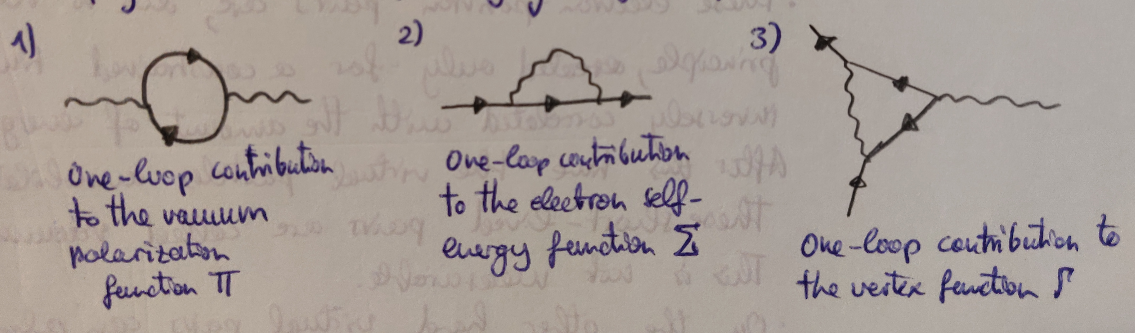
\includegraphics[width=0.7\linewidth]{gfx/DivergingIntegralsQED}
	\caption{\itshape Diverging integrals in QED appearing higher than tree level.}
	\label{fig:divergingintegralsqed}
\end{figure}
A theory is renormalizable, thus meaningful after renormalization, if the number of diverging diagrams is finite. The reason for this is that to get observables renormalized one needs a finite number of constants to maintain the predictive value of the theory untouched.
\subsubsection{Corrections to the fermion propagator}
Taking QED interactions into account the Feynman propagator $S_F(x-y)= \feynmandiagram[horizontal=a to b]{a [particle=y]-- [fermion] b [particle=x] };$ is corrected like
\begin{align}
	\expval{\hat{T}\{\psi(x) \bar{\psi}(y)\}}{\Omega} &=
	\feynmandiagram[horizontal=a to b]{a [particle=y] --c-- [fermion] b[particle=x]}; 
	+ \feynmandiagram[horizontal=a to b]{a [particle=y]--c--[fermion] d--b [particle=x], c--[boson, half left] d };\nonumber \\
	&	+\feynmandiagram[horizontal=a to b]{ a[particle=y] --c--[fermion] d -- e--f--[fermion] g--b[particle=x],
	c--[half left, boson]g, d -- [half left, boson ]f   } ; \\
&= 
\feynmandiagram[horizontal=a to b]{a[particle=y] -- c [blob] -- b [particle=x] };.
\end{align}

\begin{mybox}{Electron self-energy}
	Let 
	\begin{equation}
	\feynmandiagram[horizontal=a to b] {a [particle=A]--c [particle=$\left(1PI\right)$]--b[particle=B]  }; \equiv - i \sum(\slashed{p})_{AB}
	\end{equation}
	denote the amputated $1PI$ diagram. $\sum(\slashed{p})$ \emph{is called self-energy of the electron.}
	$\Rightarrow$ 
	\begin{align}
		\expval{\hat{T}\{\psi(x) \bar{\psi}(y) \}}{\Omega} &= \feynmandiagram[horizontal=a to b]{a[particle=y] --c--[fermion] b[particle=x] };
		+ \feynmandiagram[horizontal=a to b]{a--[fermion] c [particle=$\left(\sum\right)$]--[fermion] b  }; \nonumber \\
		&+ \feynmandiagram[horizontal=a to b]{a --[fermion]c[particle=$\left(\sum\right)$ ]--[fermion] d[particle=$\left(\sum\right)$] --[fermion]b  }; + \dots
	\end{align}
\end{mybox}
Where the full Feynman propagator for interacting QED theory takes the form (via Dyson resummation) 
\begin{equation}
\feynmandiagram[horizontal=a to b]{a [particle=y] --c [blob] -- b[particle=x]  };
= \int \frac{\md^4 p}{(2 \pi)^4} e^{-i p\cdot (x-y)} \; \frac{i}{\gamma \cdot p-m_0 - \sum(\slashed{p})+i \epsilon }.
\end{equation}



\subsubsection{Corrections to the photon propagator}
\begin{mybox}{Photon self-energy}
The Fourier transform of the photon propagator, denoted by $\feynmandiagram[horizontal=a to b]{a --[boson] c [blob] --[boson]b};$, can be derived via Dyson resummation from the $1PI$ diagram 
\begin{equation}
\feynmandiagram[horizontal=a to b]{a[particle=$\mu$] -- [boson] c -- [boson] b[particle=$\nu$] };
\equiv i \Pi^{\mu \nu} (q^2) = 
\end{equation}
which is the \emph{self-energy of the photon or vacuum polarization}.
\end{mybox}
Vacuum polarization describes the process in which a background electromagnetic field produces virtual electron-positron pairs that change the distribution of charges and currents that generated the original electromagnetic field. It is also referred to as the \emph{self-energy of the gauge boson(photon)}.\\
\\
These electron-positron pairs are, due to Heisenberg's uncertainty principle, created only for a constrained time, having duration inversely correlated with the amount of energy of the fluctuation. After this time the virtual particles annihilate each other. These short-lived pairs are called \emph{vacuum bubbles}. This is not measurable.\\
On the other hand virtual pairs can also occur as a photon progress, as seen in \ref{fig:divergingintegralsqed}; the effect on other processes is measurable.\\
$\Rightarrow$ Such charged pairs act as an electric dipole. In the presence of an electric field, e.g. the electromagnetic field around an electron, these particle-antiparticle pairs reposition themselves, thus partially counteracting the field.\\
The field therefore will be weaker than would be expected if the vacuum were completely empty. This reorientation of the short-lived particle-antiparticle pairs is referred to as  \emph{vacuum polarization}.

\subsubsection{Corrections to the interaction vertex}
\begin{mybox}{Vertex function}
	We define an effective vertex by summing up all loop-corrections. This is the \emph{vertex function} $\Gamma$, which describes the coupling between a photon and an electron beyond leading order, it is the one particle irreducible correlation function which involves $ \psi, \bar{\psi}$ and $A_{\mu}$:

\end{mybox}
	
\begin{figure}
	\centering
	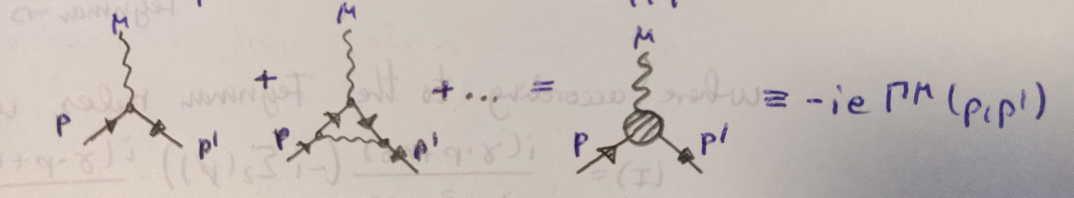
\includegraphics[width=0.7\linewidth]{gfx/VertexFunctionQED}
	\caption{\itshape Definition of the vertex function, summing up all loop corrections.}
	\label{fig:vertexfunctionqed}
\end{figure}
We will compute these corrections to 1-loop order. The diagrams will exhibit:
\begin{enumerate}
	\item Ultraviolet (UV) divergences from integrating the momenta of particles in the loop up to infinity.
	\item Infra-red (IR) divergences if the diagram contains massless particles (i.e. photons) running in the loop
\end{enumerate}
The general status of these divergences is as follows
\begin{enumerate}
	\item UV divergences require regularization of the integral and can be absorbed in a clever definition of the parameters via renormalization.
	\item IR divergences in loop-diagrams cancel if physical observables are computed.
\end{enumerate}



\subsection{Self-energy of the electron at 1-loop}
At 1-loop order the electron propagator takes the form 
\begin{equation}
	 \expval{\hat{T}\{\psi(x) \bar{\psi}(y)\}}{\Omega} =
	 \feynmandiagram[horizontal=a to b]{a [particle=y] -- [fermion] c-- b [particle=y]};
	 + \underbrace{\feynmandiagram[horizontal=a to b]{a[particle=y] --[fermion] c-- b[particle=x]}; }_{\stackrel{Feynman}{\Rightarrow} \int \frac{\md^4 p}{(2 \pi)^4} e^{-i p(x-y) } \cdot (I) }
\end{equation}
where according to the Feynman rules we have
\begin{equation}
	(I) = \frac{i(\gamma \cdot p +m_0)}{p^2-m^2_0+i \epsilon} \left(-i \sum_2(\slashed{p})\right) \frac{i(\gamma \cdot p+m_0)}{p^2-m^2_0 +i\epsilon}.
\end{equation}
$\Rightarrow$ The amputated 1-loop contribution corresponds to omitting the two outer fermion propagators and is thus given by:
\begin{equation}
	-i \sum_2(\slashed{p}) = (-i e)^2 \int \frac{\md^4 k}{(2 \pi)^4} \gamma^{\mu} \frac{i(\slashed{k}+m_0)}{k^2-m^2_0+i \epsilon} \gamma^{\nu} \frac{(-i \eta_{\mu \nu})}{(p-k)^2 + i \epsilon}.
\end{equation}
This integral has a IR-divergence near $k=0$ if $p\rightarrow0$. We will introduce a fictitious small photon mass $\mu$ to regulate the IR divergence:
\begin{equation}
	\Rightarrow i \sum_2(\slashed{p}) = (-ie)^2 \int \frac{\md^4 k}{(2 \pi)^4} \gamma^{\mu} \frac{i (\slashed{k}+m_0)}{k^2-m^2_0 +i \epsilon} \gamma_{\mu} \frac{-i}{(p-k)^2-\mu^2+i \epsilon}.
\end{equation}
The evaluation of such typical momentum integrals proceeds in 3 steps.
\subsubsection{Step 1: Feynman parameters}
The integrand contains a fraction of the form $\frac{1}{AB}$ with $A=(p-k)^2-\mu^2+i \epsilon$ and $B=k^2-m^2_0+i\epsilon$. Any $A,B \in \mathbb{C}\ \{0\}$ satisfies
\begin{equation}
	\frac{1}{AB} = \int_0^1 \md x \quad \frac{1}{\left[xA+(1-x) B\right]^2} 
\end{equation}
with $x:$ Feynman parameter. \\
$\Rightarrow$ in our case applying the identity with some algebra yields
\begin{equation}
	\frac{1}{AB} = \int_0^1  \md x \; \frac{1}{[l^2- \Delta+i \epsilon]^2}, \; l=k-xp,\; \Delta=-x(1-x) p^2+x \mu^2 +(1-x) m^2_0.
\end{equation}
With some more Dirac algebra manipulations we find
\begin{equation}
	-i \sum_2(\slashed{p}) = -e^2 \int_0^1 \md x \int \frac{\md^4 l}{(2 \pi)^4} \; \frac{-2 \slashed{p} +4 m_0}{[l^2-\Delta+i\epsilon]^2}.
\end{equation}

\subsubsection{Step 2: Wick rotation}
The Wick rotation relates typical integrals appearing in loops like $\int \frac{\md^4 l}{(2 \pi)^4} \frac{1}{[l^2-\Delta +i\epsilon]^n}$ to Euclidean integrals.\\
The $^0$ integral is in fact a complex contour integral along the real axis. The value of this integral is unchanged if we deform the contour without hitting any pole. Therefore we can rotate the contour by $90^°$ counter-clockwise to lie along the imaginary axis:
\begin{figure}
	\centering
	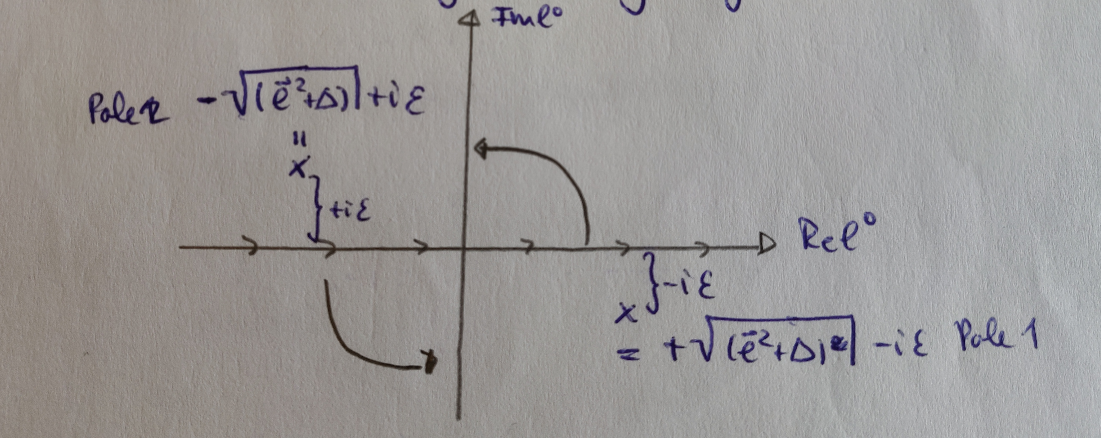
\includegraphics[width=0.7\linewidth]{gfx/Wickrotation}
	\caption{\itshape How to perform integral in the renormalization procedure by a Wick rotation.}
	\label{fig:wickrotation}
\end{figure}
Introducing the Euclidean 4-momentum $l_E = (l^0_E, \vec{l}_E)$ as 
\begin{equation}
	l^0=i l^0_E, \; \vec{l}=\vec{l}_E \; \Rightarrow \; l^2=-l^2_E\equiv \; -i \sum_j (l^j_E)^2
\end{equation}
we can write the integral as
\begin{equation}
	\int \frac{\md^4 l}{(2 \pi)^4} \, \frac{1}{[l^2-\Delta+i\epsilon]^m} = (-1)^m i \int \frac{\md^4 l}{(2 \pi)^4} \, \frac{1}{[l^2_E+\Delta - i \epsilon]^m}.
\end{equation}
Since we won't need the $i\epsilon$ any longer we can omit it at this stage. We can now perform the integral as a spherical integral in $\mR^4$.































\chapter{Advanced Quantum Field Theory}
\section{Path Integral Quantization}
\subsection{Path integral in Quantum Mechanics}
The path integral provides a formulation of quantum theory completely equivalent to the canonical quantization.\\
\\
A quantum mechanical transition amplitude $\braket{q_f,t_f}{q_i,t_i} = \bra{q_f} e^{i \hat{H}(t_f-t_i)} \ket{q_i}$ can, by partitioning of the \emph{transition time} $\delta t=\frac{t_f-t_i}{N+1}$ and insertion of \emph{complete sets of states} $\mathcal{I}= \int_{\mR} \md q_k \, \ket{q_k}\bra{q_k}$ between each partition, be expressed as 
\begin{equation}
	\braket{q_f,t_f}{q_i,t_i} = \lim_{N\rightarrow\infty} \int \frac{\md p_0}{2 \pi} \prod_{k=1}^{N} \frac{\md p_k \md q_k}{2 \pi} \exp\left[i \sum_{k=0}^{N} \left(p_k \frac{q_{k+1}-q_k}{\delta t} - H\right) \delta t\right]
\end{equation}
\marginpar{Thus, we have boundary conditions for $q(t)$, whereas $p(t)$ is free at the endpoints.}
which is per definition equivalent to
\begin{equation}
	\braket{q_f,t_f}{q_i,t_i} = \int_{q(t_i)=q_i}^{q(t_f)=q_f}  \mathcal{D}q(t) \mathcal{D}p(t) \, \exp\left[i\int_{t_i}^{t_f} \md t \left(p \dot{q} - H(p,q) \right)\right]
\end{equation}
with 
\begin{equation}
	S[p,q] \equiv \int_{t_i}^{t_f} \md t \; L(p,q) \quad \mathrm{and} \quad L(p,q) \equiv p \dot{q} - H(p,q)
\end{equation}
which holds true for every Weyl-ordered Hamiltonian, e.g. $H=f(p)+V(q)$.\\
\begin{mybox}{Feynman path integral}
	\emph{Analytic continuation} by rotating $t$ onto the lower half-plane via $\delta t \rightarrow \delta t (1-i \epsilon)$ followed by performing the momentum path integral as a Gaussian yields the Feynman-Kac formula
	\begin{equation}
		\braket{q_f,t_f}{q_i,t_i} = \lim_{N\rightarrow\infty} C^{N+1} \prod_{k=1}^{N} \int \md q_k \, e^{i \int_{t_i}^{t_f} \md t \, L(q,\dot{q})}= \int_{q(t_i)=q_i}^{q(t_f)=q_f} \mathcal{D}q(t) e^{i \int_{t_i}^{t_f} \md t\, L(q,\dot{q})}
	\end{equation}
	where the factor $C^{N+1} = \left(\frac{-i m}{2 \pi \delta t}\right)^{\frac{N+1}{2}}$ is absorbed into $\mathcal{D}q(t)$, using $C:= \sqrt{\frac{-im}{2 \pi \delta t}}$.s
\end{mybox}
This is interpreted as:\\
The transition amplitude $\braket{q_f,t_f}{q_i,t_i}$ counts all possible continuous path from $q_i$ to $q_f$ weighted by $\exp\left[\frac{i}{\hbar} S\right]$. In the \emph{classical limit} $S[q,\dot{q}] \gg \hbar$ and due to the strongly oscillating phase of the integrand, the right-hand side is dominated by paths for which the action becomes \emph{stationary}
\begin{equation}
	\frac{\delta S}{\delta q} =0 \quad \Leftrightarrow \; \mathrm{principle\,of\,least\, action}.
\end{equation}
This is the \emph{classical path}, quantum physics is obtained by summing up all additionally possible paths with the classical path via the path integral.\\
\\
The limit $N\rightarrow\infty$ and the ensuing interpretation of the path integral as an integral over all continuous paths from $q_i$ to $q_f$ can be made mathematically rigorous - at least for $H=\frac{p^2}{2m} +V(q)$ -by passing to the Euclidean theory.\\
\\
\begin{mybox}{N-point correlators}
	For n-point correlation functions we find in the interacting theory, that the time ordering appears automatically, which means that under the path-integral the operators are merely $\mathbb{C}$-numbers, such that ordering is not necessary anymore:
	\begin{equation}
		\expval{\hat{T}\prod_i \hat{q}_H(t_i) }{\Omega} = \lim_{T\rightarrow \infty(1-i \epsilon)} \frac{\int \mathcal{D}q(t) \mathcal{D}p(t) e^{-i \int_{-T}^{T} \md t L(p,q)} \prod_i q(t_i ) }{\int \mathcal{D}q(t) \mathcal{D}p(t) e^{i \int_{-T}^T \md t L(p,q)} }.
	\end{equation}
\end{mybox}

\subsection{The path integral for scalar fields}
\begin{mybox}{Path integral of a real scalar field}
The path integral for real scalar fields $\phi(x)$ (as opposed to particles) is given by
\begin{equation}
	\braket{\phi_f(\vec{x} ),t_f }{\phi_i(\vec{x}),t_i} = \int_{\phi(\vec{x},t_i) = \phi_i(\vec{x})}^{\phi(\vec{x},t_f)=\phi_f(\vec{x})} \mathcal{D}\phi(x) e^{i \int_{t_i}^{t_f} \md t \int_{\mR^3} \md^3 x \mL[\phi(x)]}.
\end{equation}
\end{mybox}
\begin{mybox}{Master formula for cumulants}
	The master formula for an n-point quantum correlation function reads
	\begin{align}
		G(x_1,\dots,x_n) &= \expval{\hat{T} \prod_{j=1}^{n} \hat{\phi}_H(x_j) }{\Omega} \nonumber\\
		&= \lim_{T\rightarrow\infty(1-i\epsilon)} \frac{\int \mathcal{D}\phi(x) \prod_{j=1}^{n} \phi(x_j) e^{-i \int_{-T}^T \md^4 x \mL(\phi)(x) } }{\int \mathcal{D}\phi(x) e^{i \int_{-T}^T \md^4 x \mL [\phi(x)]}}.
	\end{align}
\end{mybox}
In a perturbatively renormalizabe theory, the action can be renormalized order by order such that the perturbatively expanded correlation functions are finite in the continuum limit, order by order. One can evaluate the path-integral in an exact, non-perturbative manner by e.g. \emph{Lattice Field Theory} (c.f. page 181).








\subsection{Generating Functional for Correlation Functions}
\begin{mybox}{Generating functional}
	The generating functional $Z[J]$ of Green's functions $G(x_1, \dots, x_n)$ for some source $J(x)$ reads
	\begin{equation}
	Z[J] = \int \mathcal{D}\phi \; e^{i S[\phi] + i J \cdot \phi },
	\end{equation}
	where the functional inner product is defined as
	\begin{equation}
	J \cdot \phi = \int_{\mR^{3,1}} \md^4 x J(x)\phi(x).
	\end{equation}
\end{mybox}
$Z[J]$ maps the function $\phi(x)$ to a number in $\mathbb{C}$. It is called generating functional because
\begin{equation}
\frac{Z[J]}{Z[0]} = \sum_{n=0}^{\infty} \frac{i^n}{n!} \left(\prod_{j=1}^{n} \int_{\mR^{3,1}} \md^4 x_j \, J(x_j) \right)G(x_1,\dots,x_n).
\end{equation}

\begin{mybox}{Calculating cumulants from the generating functional}
	This can be solved for $G(x_1,\dots,x_n)$ using the tools of functional calculus:
	\begin{equation}
	G(x_1,\dots,x_n) = \frac{1}{Z[0]} \left[\prod_{j=1}^{n} \frac{\delta}{i \delta J(x_j)}\right] Z[J] |_{J=0},
	\end{equation}
	with the functional derivative
	\begin{equation}
	\frac{\delta \phi(y) }{\delta \phi(x)} = \delta_D(x-y).
	\end{equation}
\end{mybox}
$Z[0]$ contains no external points and represents the partition function $Z[0]=e^{\sum_i V_i}$, where the sum runs over all vacuum bubbles $V_i$ of the theory. Consequently, $\frac{Z[J]}{Z[0]}$ contains no vacuum bubbles.







\subsection{Perturbative Expansion in Interacting Theory}
$Z_0[0]$ is in general a divergent quantity, but i can be rigorously defined by a regularization procedure.\\
All physical quantities are computed in the regularized theory and the expression $Z_0[0]$ cancels in all such expressions because the correlation functions derive from $\frac{Z[J]}{Z[0]}$.\\
To compute a $2n$-point function one expands the exponential precisely to $n$-th order, while the $2n+1$-functions vanish.\\
\\
Consider an action with an interaction
\begin{align}
	S[\phi] &= S_0 [\phi] \quad + \int_{\mR^{3,1}} \md^4 x \, \mL_{int} [\phi] \\
	\Rightarrow Z[J] &= \exp\left[i \int_{\mR^{3,1}} \md^4 x \, \mL_{int} \left[- \frac{i \delta}{\delta J} \right]   \right] Z_0[J].
\end{align}

\begin{mybox}{Wick theorem in path integral language}
	We can recover the Feynman rules and Wick's theorem equivalently as in the canonical quantization with the definition for function $F[\phi]$
	\begin{equation}
		\langle F[\phi] \rangle_0 := e^{\half \frac{\delta}{\delta \phi} \cdot D_F \cdot \frac{\delta}{\delta \phi }} F[\phi] |_{\phi=0}
	\end{equation}
	with the scalar Feynman propagator $D_F$, such that the following hold true for \emph{scalar} theories:
	\begin{equation}
		\Rightarrow G(x_1,\dots ,x_n) : \frac{\langle \phi(x_1) \dots \phi(x_n) \exp\left[i \int \md^4 x \mL_{int}\right] \rangle_0}{\langle \exp(\left[i \int \md^4 x \mL_{int} \right] \rangle _0)}.
	\end{equation}
	We can identify :
	\begin{equation}
		\langle \phi(x_1) \phi(x_2) \rangle_0 = \expval{\hat{T} \hat{\phi}(x_1) \hat{\phi}(x_2)}{0} = \contraction{}{\phi(x_1)}{}{\phi(x_2)} \phi(x_1) \phi(x_2),
	\end{equation}
	which gives us the results of Wick's theorem
	\begin{align}
		\langle \phi_1 \dots \phi_{2n} \rangle_0 = \contraction{}{\phi_1}{}{\phi_2} \phi_1 \phi_2 \contraction{}{\phi_3}{}{\phi_4} \phi_3 \phi_4 \dots \contraction{}{\phi_{2n-1}}{}{\phi_{2n}}  \phi_{2n-1} \phi_{2n} \nonumber \\
		&+ all other contractions.\\
		\langle \phi_1 \dots \phi_{2n+1} \rangle_0 &=0.
	\end{align}
\end{mybox}
With Wick's theorem at hand we recover the exact same Feynman rules as in operator language from the Gell-Mann-Low formula in the interaction picture for position and momentum space.\\
Note, that $\phi(x_i)$ or $\frac{\delta}{i \delta J(x_i)}$ corresponds to an external point in the Feynman diagram, that a line between $x_i$ and $x_j$ denotes as always a factor $D_F(x_i-x_j)$ :
\begin{equation}
	\feynmandiagram[horizontal=a to b] {a[particle=$x_i$] --c -- [fermion] d[edge label=$D_F(x_i-x_j)$]-- b[particle=$x_j$]};
\end{equation}
and that interactions only occur if there is a dot on crossing lines:
\begin{equation}
	\feynmandiagram[horizontal=a to b]{a[particle=$x_1$]  --[fermion] z [dot] -- [anti fermion] b [particle=$x_2$],
	c [particle=$x_3$] -- [fermion] z -- [anti fermion] d [particle=$x_4$]   };
\end{equation}

\subsubsection{On the counting of loops}
A fully connected Feynman diagram in momentum space with $E$ external and $I$ internal lines, $V$ vertices, and $L$ loops (number of unfixed momentum integrals) satisfies \emph{Euler's formla}
\begin{equation}
	L = I-V+1 \; \leftrightarrow \; \underbrace{\feynmandiagram[horizontal=a to b] {a[particle=$x_i$] -- c [dot] --[half left] d [dot] -- b [particle=$x_j$] , d--[half right] c  };				}_{1= 2-2+1}
\end{equation}
$\Rightarrow$ For $\mL_{int}(\phi) = \frac{\lambda^n}{n!} \phi^n(x)$ we have
\begin{equation}
	E + 2 I \quad = \quad nV,
\end{equation}
because every vertex connects to $n$ lines, while every external line connects to one and every internal line to two vertices. Together with Euler's formula we have
\begin{equation}
	(n-2)V \quad = 2L + (E-2).
\end{equation}
Hence for fixed $E$, an expansion in $L$ corresponds to an expansion in $V$.




\subsection{The Schwinger-Dyson Equation}
\begin{mybox}{Symmetries in path integral language}
	An advantage of the path-integral method is that symmetries are more transparent. It becomes clear that classical symmetries carry over to the quantum theory -  but only provided the path integral measure $\mathcal{D}\phi =\mathcal{D}\phi'$ is invariant under a given transformation corresponding to the symmetry. In that case, the Schwinger-Dyson equation
	\begin{align}
		\left(\frac{\delta S}{\delta \phi} |_{\phi=\frac{\delta}{i \delta J}} + J\right) Z[J] &= 0\\
		&= \int \mathcal{D}\phi \left[\frac{\delta S}{\delta \phi(x)} + J(x) \right] e^{i\left(S[\phi] + J \cdot \phi \right)}
	\end{align}
states that the classical equation of motion (in presence of a source $J$)
\begin{equation}
	0 = \frac{\delta S}{\delta \phi} + J
\end{equation}
holds as an operator equation in the quantum theory, i.e. it holds inside the path integral. They provide the e.p.m. for Green's functions/ for given n-point correlators. Note that these equations of motion are therefore preserved under the transformation $\phi \rightarrow\phi'$.
\end{mybox}
Note that this is only true as long as there are no contact terms $\propto \delta_D(x-x_j)$.\\
$\Rightarrow$ The idea is that the interactions of a theory are also represented in its Green's functions. The full Green's functions containing the interaction should also contain the free Green's functions in the \emph{limit of the free theory.}\\
The full 1-point function can be understood in terms of full higher n-point functions and bare interactions as encoded in $S[\phi]$.\\
\\
\begin{mybox}{Ward-Takahashi identity}
For a continuous global classical symmetry $\phi \rightarrow \phi' = \phi + \delta \phi$ with conserved Noether current $j^{\mu} (x)$ given by $\frac{\delta S}{\delta \phi(x)}
\delta \phi(x) = - \partial_{\mu} j^{\mu} (x) =0$ \emph{on-shell} we can find the \emph{Ward-Takahashi identity}
\begin{align}
	&\partial_{\mu} \expval{\hat{T} j^{\mu} \prod_{i=1}^{n} \phi(x_i) }{\Omega} = \\
	&-i \sum_{i=1}^{n} \expval{\hat{T} \phi(x_1) \dots \phi(x_{i-1} \delta \phi(x) \delta^{(4)}_D(x-x_i) \phi(x_{i+1}) \dots \phi(x_n) }{\Omega}
\end{align}
which is derived from the Schwinger-Dyson equation, i.e. the statement of current conservation up to contact terms inside correlation functions.
\end{mybox}
Like the Schwinger-Dyson equation, the Ward-Takahashi identity only holds for classical symmetries of $S[\phi]$ that leave the measure invariant.\\
If $\mathcal{D}\phi$ is affected, the symmetry is \emph{anomalous} and current conservation (up to contact terms) does not hold at quantum level.


\subsection{Connected diagrams}
$G(x_1,\dots, x_n)$ receives contributions from partially connected Feynman diagrams. These are the diagrams that factor into subdiagrams each of which is connected only to some of the $n$ external points $x_1,\dots, x_n$. As established by the LSZ formalism, what enters the computation of scattering amplitudes are only the fully connected Green's functions $G^{(c)} (x_1, \dots, x_n)$ corresponding to fully connected Feynman graphs, i.e. to those Feynman diagrams which do not factor into subdiagrams. \\
$\Rightarrow$ 
\begin{mybox}{Generating functional of connected diagrams/cumulants}
	The generating functional of $G^{(c)}(x_1,\dots,x_n)$ is called \emph{effective action}  and denoted by $i W[J]$. It is given by 
	\begin{equation}
		\frac{Z[J]}{Z[0]} = e^{i W[J]}
	\end{equation}
	Thus,
	\begin{align}
		\tau(x_1,\dots,x_n) &= \frac{\delta}{i \delta J(x_1)} \dots \frac{\delta}{i \delta J(x_n)} i W[J] \\
		&\Rightarrow \quad G^{(c)}(x_1,\dots ,x_n) &= \tau (x_1, \dots,x_n) |_{J=0}.
	\end{align}
	\end{mybox}
Summarizing,
\begin{enumerate}
\item $G^{(c)}=$ cumulants.
\item  $\tau(x_1,\dots,x_n)$ denotes a fully connected n-point Green's function in the presence of a source $J$. The fully connected are a subset of all Green's functions.
\item \begin{mybox}{$1PI$ effective action}
	An even stronger reduction are the fully connected, amputated $1PI$ Green's functions $\tilde{\Gamma}(x_1, \dots,x_n)$ in the presence of the field $\varphi \left(\Gamma(x_1,\dots,x_n) = \tilde{\Gamma}(x_1,\dots,x_n)|_{\varphi=0}	\right)$ generated by the $1PI$ effective action $\Gamma[\varphi]$.
	\end{mybox}
\end{enumerate} 




\subsection{The $1PI$ effective action}
\begin{mybox}{Effective action, general idea}
	In QFT, the effective action is a modified expression for the action, which takes into account quantum-mechanical corrections in the following sense: \\
	In classical mechanics, the equation of motion can be derived from the principle of least action. This is not the case in QM, where the amplitudes of all possible motions are added up in the path integral. However, if the action is replaced by the effective action, the equation of motion for the vacuum expectation value of the field 
	\begin{equation}
		\varphi = \langle \phi \rangle 
	\end{equation}
	can be derived from the requirement that the effective action be stationary.
\end{mybox}
An important subclass of fully connected Feynman diagrams are the 1-particle-irreducible ($1PI$) diagrams, which cannot be cut into two non-trivial diagrams by cutting a single (internal) line.\\
\begin{mybox}{$1PI$ effective action}
The generating function for the $1PI$ connected diagrams is called the \emph{$1PI$ effective action} $\Gamma[\varphi]$, which is defined as the Legendre transform of $W[J]$:
\begin{equation}
	\Gamma[\varphi] := W[J_{\varphi} ] - \varphi \cdot J_{\varphi} \equiv W[J_{\varphi}] - \int \md^4 x' \varphi(x' ) J_{\varphi}(x' )
	\end{equation}
	where $\varphi(x)$ is the 1-point function of $phi(x)$ in the presence of a source $J$ 
	\begin{equation}
		\varphi(x) \equiv \frac{\delta W[J]}{\delta J(x)} = \expval{\hat{\phi}(x)}{\Omega}_J = \mathrm{vacuum\,expectation\,value}
	\end{equation}
	and we assumed there to be a bijection between $J$ and $\varphi$.
\end{mybox}
$\Gamma[\varphi]$ is now also the generating functional for the $1PI$ connected amputated Green's  functions $\Gamma_n(x_1,\dots,x_n)$,
 \begin{equation}
 	i \Gamma [\varphi] = \sum_{n=0}^{\infty } \frac{1}{n!} \int \md^4 x_1 \dots \md^4 x_n \varphi(x_1) \dots \varphi(x_n) \Gamma_n(x_1,\dots,x_n).
 \end{equation}
 Now, $\Gamma_n(x_i), n\geq 3$, is the sum of the tree-level vertex plus of the 1- and higher-loop $1PI$ amputated corrections, while $\Gamma_2(x_1,x_2)$ consists of the 1- and higher loop $1PI$ amputated diagrams minus the tree-level propagator.\\
 \begin{mybox}{Connected diagrams in the full quantum theory}
 	To compute a connected n-point function in the full quantum theory, we use the tree-level Feynman rules but replace each $k$-vertex (with $k\geq 3$) of the classical action $S[\phi]$ with the $1PI$ amputated $k$-vertex $\Gamma_k$ as encoded in $\Gamma[\varphi]$ and replace the free propagator with $G_2$, the \emph{fully resummed propagator}.\\
 	\\
 	$\Rightarrow$ Replacing $S[\phi]$ by $\Gamma[\varphi]$ and computing at tree-level gives the full quantum theory. Gives classical equation of motion as provided by $S[\phi] +$ additional quantum mechanical corrections.\\
 	\\
 	$\Gamma[\varphi]$ and $S[\phi]$ are the same functionals at tree-level, i.e. 
 	\begin{equation}
 		\Gamma[\varphi] = S[\varphi] \quad + \hbar K[\varphi] 
 	\end{equation}
 	for some $K[\varphi]$ starting at one-loop. The equation
 	\begin{equation}
 		\frac{\delta \Gamma [\varphi]}{\delta \varphi(x)} = - J(x), \; i.e. \frac{\delta \Gamma[\varphi]}{\delta \varphi(x)} = 0, \quad for \; J(x) =0
 	\end{equation}
 	is the \emph{quantum effective equation of motion} replacing $\frac{\delta S}{\delta \phi}=0$ in the full quantum theory.\\
 	The quantum mechanical corrections start at 1-loop; before, the full theory is provided by $\frac{\delta S}{\delta \phi}=0$.
 \end{mybox}


\subsection{Background Field Method}
\begin{mybox}{Background field method in QFT:}
A general field can be decomposed into the vacuum expectation value of the quantum operator $\hat{\phi}(x)$, thus $\varphi(x)$, and the \emph{quantum fluctuation} $f(x)$ around the \emph{background} $\varphi(x)$:
\begin{equation}
	\phi(x) = \varphi(x) \quad + f(x).
\end{equation}
The $1PI$-effective action is then obtained by integrating out the vacuum fluctuations
\begin{align}
	\Gamma[\varphi] &= S[\varphi] \nonumber \\
	&-i  \hbar \ln\left[\int \tilde{\mathcal{D}}f \exp\left\{ \frac{i}{\hbar } \left(\half f \cdot \frac{\delta^2 S}{\delta \varphi^2} \cdot f-\hbar \frac{\delta K}{\delta \varphi} \cdot f + \mathcal{O}(f^3) \right)    \right\}\right] \\
	&\equiv S[\varphi] \quad + \hbar K[\varphi].
\end{align}
\end{mybox}
This can be solved perturbatively
\begin{equation}
	\Gamma[\varphi] = S[\varphi] + \hbar K^{(1-loop)} [\varphi] + \mathrm{higher-loop \, corrections}
\end{equation}
with 
\begin{equation}
	K^{(1-loop)} [\varphi] = -i \ln\left[\tilde{\mathcal{D}}f \exp \left\{- \half f\cdot \left(- \frac{i}{\hbar} \frac{\delta^2 S}{\delta \varphi^2}\right)\cdot f \right\}\right].
\end{equation}
This way one can already solve the whole theory up to $x$-loops perturbatively, if quantum fluctuations and action are known.


\subsection{Grassman algebra calculus}
Fermionic anticommutation relations $\{\hat{\psi}^A(t,\vec{x}), \hat{\psi}^{\dagger}_B(t,\vec{y})  \} = \delta^A_B \delta^{(3)}_D(\vec{x}-\vec{y}), \{\hat{\psi}^A(t,\vec{x}), \hat{\psi}_B(t,\vec{y}) \}=0=\{\hat{\psi}^{\dagger}_A(t,\vec{x}), \hat{\psi}^{\dagger}_B(t,\vec{y})  \}$ can be implemented into the path integral formalism by using anticommuting, nilpotent, Grassman-valued fields $\psi(x)$ out of a Grassmann algebra $\mathbb{A}$. This is the case, because these anticommutation reltaions imply the need for \emph{anti-commuting numbers}, thus
\begin{equation}
	\psi^A_i(t)\psi^B_j(t) = - \psi^B_J(t) \psi^A_i(t),
\end{equation}
these $\psi_i$ take values in a so-called Grassmann-algebra $\mathbb{A}$ defined as follows:
\begin{enumerate}
\item Let $\theta_i, i=1,\dots,n$ be a basis of an n-dimensional complex vector space $V$, i.e. we have the notion of scalar multiplication $a \theta_i = \theta_i a$, $a\in \mathbb{C}$ and vector addition $a \theta_i+b \theta_j \in V$.
\item Define then a bilinear anti-commutative multiplication
\begin{equation}
	\theta_i \theta_j = - \theta_j \theta_i
\end{equation}
as a map from $V\times V\mapsto \Lambda^2 V$, where $\Lambda^2 V$ is the antisymmetric tensor product of $V$.
\item Iteratively we can build higher rank anti-symmetric product spaces $\Lambda^kV$ up to $\Lambda^n V$.
\item Then the Grassman (or exterior) algebra is defined as the space
\begin{equation}
	\mathbb{A} = \bigoplus_{k=0}^n \Lambda^k V = \mathbb{C} \oplus V \oplus \Lambda^2 V \oplus \dots \oplus \Lambda^n V.
\end{equation}
A typical element of $\mathbb{A}$ is of the form
\begin{equation}
	a + a_i \theta_i + \half a_{ij} \theta_i  \theta_j + \dots + \frac{1}{n!} a_{i_1 \dots i_n} \theta_{i_1} \dots \theta_{i_n}.
\end{equation}
\item The coefficients are completely antisymmetric $a_{ij}=-a_{ji}$. The elements of the abstract Grassmann algebra $\mathbb{A}, \theta_i$ namely, are called Grassmann numbers and they are \emph{nilpotent}:
\begin{equation}
	\theta^2_i = 0.
\end{equation}
$\Rightarrow$ An important example of a Grassmann algebra is the space $\Omega$ of differential forms defined on an $n$-dimensional manifold endowed with the structure wedge (or exterior product) (compare Differential geometry section 1.2 under GR).
\item A Grassmann algebra is a graded algebra:
\begin{enumerate}
	\item An element of $\Lambda^{2k}V$ has grade (or degree) $s=0$ (even).
	\item An element of $\Lambda^{2k+1}V$ has grade (or degree) $s=1$ (odd).
\end{enumerate}
$\Rightarrow$ Note that a general element of $\mathbb{A}$ can always be written as the sum of an even and an odd element.
\item Two elements $A,B\in  \mathbb{A}$ of definite $s_A$ and $s_B$ satisfy
\begin{equation}
	AB= (-1)^{s_A s_B} BA.
\end{equation}
Thus, even elements are commuting and therefore sometimes called bosonic, whereas odd elements are dubbed fermionic due to their anti-commuting nature.
\item To set up a notion of calculus on the space of functions
\begin{equation}
	f:\mathbb{A} \rightarrow \mathbb{C}, \underbar{\theta} \mapsto f(\underbar{\theta}) = a + a_i \theta_i+\dots + \frac{1}{n!} a_{i_1 \dots i_n} \theta_{i_1} \dots \theta_{i_n}
\end{equation}
one defines differentiation w.r.t. $\theta_i$ as follows:
\begin{enumerate}
	\item \begin{equation}
		\frac{\partial}{\partial \theta_i} \theta_j = \delta_{ij}, \quad \frac{\partial}{\partial \theta_j} a= 0 \; \forall a\in \mathbb{C},
	\end{equation}
	\item \begin{equation}
		\frac{\partial}{\partial \theta_i} \left[a_1 f_1(\underbar{\theta}) + a_2 f_2(\underbar{\theta}) \right] = a_1 \frac{\partial}{\partial \theta_i} f_1(\underbar{\theta}) + a_2 \frac{\partial}{\partial \theta_i} f_2(\underbar{\theta}) \; Linearity
	\end{equation}
	\item If $f_1(\underbar{\theta})$ has definite grade $s$, then the graded Leibniz rule holds
	\begin{equation}
		\frac{\partial}{\partial \theta_i} \left[f_1(\underbar{\theta})f_2(\underbar{\theta}) \right] = \left(\frac{\partial}{\partial \theta_i} f_1(\underbar{\theta})\right)f_2(\underbar{\theta}) + (-1)^s f_1(\underbar{\theta}) \frac{\partial}{\partial \theta_i} f_2(\underbar{\theta}).
	\end{equation}
\end{enumerate}
\item We define an integral $I[f(\underbar{\theta })]$ as a functional of $f(\underbar{\theta})$. Consider first a Grassmann algebra with $n=1: \mathbb{A}=\mathbb{C} \oplus V:$
\begin{equation}
	I[f(\theta)] = \int  \md \theta f(\theta) = \int \md \theta [a + b \theta].
\end{equation}
Linearity and translation hold for this integral
\begin{enumerate}
	\item Translation invariance means invariance under a shift of the integration variable $\theta \rightarrow \theta +C$, this implies 
	\begin{align}
		\int \md \theta C &= 0\quad \forall C\in \mathbb{C}  \quad Normalize \; \int \md\theta \theta =1\\
		\Rightarrow \int \md \theta [a + b \theta] &= b = \frac{\partial}{\partial \theta } [a +b \theta] \\
		\Rightarrow ! \int \md \theta_i \theta_j &= \delta_{ij} = \frac{\partial}{\partial \theta_i} \theta_j..
	\end{align}
\item The general Grassmann measure is defined as 
\begin{align}
	\md^n \theta & := \md \theta_n \md \theta_{n-1} \dots \md \theta_1, \mathrm{with\,order}  \md \theta_i \md \theta_j = - \md \theta_j \md \theta_i \\
	\Rightarrow & \int \md^n \theta \theta_{i_1} \dots \theta_{i_n} = \epsilon_{i_1 \dots i_n} \\
	\Rightarrow  & \int \md^n \theta f(\underbar{\theta}) = \frac{1}{n!} a_{i_1 \dots i_n} \epsilon_{i_1 \dots i_n} = a_{123\dots n}
\end{align}
Only those terms contribute for which the Grassmann integral is "saturated" such that each $\md \theta_i$ is paired with precisely are $\theta_i$.
\end{enumerate}
\item For a linear change of Grassmann integration variables we find for $A$ being an $(n\times n)$-matrix the Jacobian to be
\begin{equation}
	\underbar{\theta}' = A \underbar{\theta} \quad \Rightarrow  \quad \md^n \theta = \det A \; \md^n \theta'.
\end{equation}
\item Complexification: Consider $\theta_i$ and $\theta^*_i$ from now on as independent degrees of freedom and define the complex conjugate via
\begin{align}
	(\theta_i \theta_j)^* &= \theta^*_j \theta^*_i \\
\Rightarrow \md^n \theta \md^n \theta^* & := \md \theta_1 \md \theta^*_1 \dots \md \theta_n \md \theta^*_n.
\end{align}
\item Let us compare bosonic and fermionic Gaussian integrals:
\begin{enumerate}
	\item Real case:
	\begin{align}
		\int \md^n x e^{- \half x_i A_{ij} x_j} &= \sqrt{\frac{(2\pi)^2}{\det A}} \quad (\mathrm{bosonic \, integration}) \\
		\int \md^n \theta e^{\half \theta_i A_{ij} \theta_j } &= \sqrt{\det A} = Pf(A)  \quad (\mathrm{fermionic \, integration}).
	\end{align}
\item Complex case:
	\begin{align}
		\int \md^n z \md^n z^* e^{-z^*_i B_{ij} z_j} = \frac{(2 \pi)^n}{\det B} \quad (\mathrm{bosonic}) \\
		\int \md^n \theta^* \md^n \theta e^{- \theta^*_i B_{ij} \theta_j} = \det B \quad (fermionic).
	\end{align}
\end{enumerate}
\end{enumerate}




\subsection{The fermionic path integral}
\begin{mybox}{The fermionic path integral}
The fermionic path integral is derived in the same fashion as the bosonic one w.r.t. the anticommutation relation. Thus, partitioning of the transition time $\delta t = \frac{t_f-t_i}{N}$ and insertion of complete sets of states $\mathcal{I} = \int \md\psi^* \md \psi \ket{\psi} e^{-\psi^* \psi } \bra{\psi}$, with $\psi$ being a complex Grassmann number, leads to the path integral for Dirac fermionic fields $\psi(x)$, $\bar{\psi}(x) = \psi^{\dagger}(x) \gamma^0$
\begin{equation}
	\braket{\psi_f(\vec{x}_f), t_f}{\psi_i(\vec{x}_i),t_i} = \int_{\psi(x,t_i)=\psi_i(x)}^{\psi(x,t_f)=\psi_f(x)} \mathcal{D}\bar{\psi}(t,\vec{x}) \mathcal{D}\psi(t,\vec{x}) e^{i \int_{t_i}^{t_f} \md^4 x \, \mL (\psi, \bar{\psi})},
\end{equation}
where $\mL(\psi,\bar{\psi})=\bar{\psi}(x) [i \slashed{\partial} - m_0] \psi(x) + \mL_{int}$.
\end{mybox}
The four $n\times n$-gamma-matrices (one for every spacetime dimension) span the Clifford algebra $Cl^n(\mathbb{C})$ defined by the anticommutator
\begin{equation}
	\{\gamma^{\mu},\gamma^{\nu} \} = 2 \eta^{\mu \nu} \mathcal{I}_{4\times 4}, \quad \mathrm{with} \, n=2^{d/2} = 4.
\end{equation}
To project initial and final states to the interacting vacuum $\ket{\Omega}$, the trick $m_0 \rightarrow m_0 - i \epsilon$ can be used.\\
\begin{mybox}{Generating functional for fermionic correlators}
	The generating functional for fermionic correlators is defined as 
	\begin{align}
		Z[\eta, \bar{\eta}] &= \expval{\hat{T} \exp\left[i \int_{\mR^{3,1}} \md^4 x \left(\mL(\psi,\bar{\psi}) + \bar{\psi}(x) \eta(x) + \bar{\eta}(x) \psi(x) \right)\right]}{\Omega} \\
		&= \int \mathcal{D}\bar{\psi} \mathcal{D}\psi \exp\left[i S[\psi, \bar{\psi}]+ i \bar{\eta} \cdot \psi + i \bar{\psi} \cdot \eta \right]
	\end{align}
with the external sources $\bar{\eta}(x), \eta(x)$ as Grassmann-valued classical fields.
\end{mybox}


\subsection{Executive Summary of QFT }
\marginpar{In Euclidean Signature.}
\begin{mybox}{Executive Summary of QFT}
Start with a classical action $S[\phi]$ in which the field $\phi(x)$ arises as the continuum limit $N\rightarrow \infty$ of a system of $N$ harmonic oscillators.\\
In the classical limit $\hbar \rightarrow 0, \phi(x)$ is a definite function given by the classical equation of motion $\frac{\delta S[\phi]}{\delta \phi(x)}=0$.
\begin{mybox}{Interpretation of the path integral}
	For $\hbar$ finite, quantum fluctuations arise. These are encoded in $Z[J]$, where the path integral takes into account all possible functions $\phi(x)$ could assume (thus classical+ quantum fluctuations).
\end{mybox}
What we can compute in the quantum theory are correlation functions. In particular, the quantum expectation value of the field $\phi(x)$ in the presence of a source $J$ is
\begin{equation}
	\varphi_J(x) := \langle \phi(x) \rangle_J = \expval{\hat{ \phi}(x) }{\Omega}_J = \frac{1}{Z[0]} \int \mathcal{D}\phi \, \phi(x) e^{- \frac{1}{\hbar} [S[\phi] + \phi \cdot J]}.
\end{equation}
With our definition of $W[J]$, we can compute this as 
\begin{equation}
	\varphi_J(x) = - \frac{\delta W[J]}{\delta J(x)}.
\end{equation}
In terms of the Légendre transform $\Gamma[\varphi]$ of $W[J]$, we have
\begin{equation}
	\frac{\delta \Gamma[\varphi]}{\delta \varphi(x)} = J(x).
\end{equation}
$\Rightarrow$ By integrating out quantum fluctuations $f(x)=\phi(x)-\varphi(x)$, $\Gamma[\varphi]$ gives a quantum effective action
\begin{equation}
	e^{- \frac{1}{\hbar} \Gamma[\varphi]} = \frac{1}{Z[0]} \int \mathcal{D}f \exp\left[-\frac{1}{\hbar} \left(S[\varphi+f] + \frac{\delta \Gamma}{\delta \varphi} \cdot f\right)\right].
\end{equation}
Replacing $S[\phi]$ by $\Gamma[\varphi]$ introduces $1PI$ amputated vertices and fully resummed propagators. Thus, computing at tree-level with $\Gamma[\varphi]$ already gives the full quantum theory !
\end{mybox}



\newpage

\section{Renormalization of QFT}

\subsection{Superficial divergence}
\begin{mybox}{Renormalizability}
	A general QFT is called renormalizable if only a finite number of resummed amputated $1PI$ diagrams is UV divergent.
\end{mybox}
Suppose the renormalizable QFT contains $m$ different fields and suppose that the UV divergent $1PI$ diagrams give rise to $n$ divergent constants order by order in perturbation theory. Then $(n-m)$ of these constants can be absorbed in the definition of $(n-m)$ unphysical parameters, the so-called \emph{bare couplings.}\\
This procedure requires specifying the outcome of $(n-m)$ physical observables as external input, i.e. experiment $\Rightarrow$ bare couplings. The remaining $m$ constants can be absorbed in the definition of the kinetic terms of the $m$ fields without reducing the predictability of the theory further. Thus in a renormalizable theory only a finite number $(n-m)$ of physical observables must be specified order by order in perturbation theory, and predictive power is retained for all remaining observables, which can e computed and are finite as we remove the cutoff.\\
However, the price to pay for the appearance of the UV divergences in the first place is that the $(n-m)$ observables cannot be computed by the theory even in principle! For instance, QED cannot make any predictions whatsoever for the absolute value of the electron mass or the charge at $q^2=0$. However, once we take $e(q^2=0)$ from experiment, QED does predict the logarithmic running of the effective charge as a function of $q^2$. As a result the renormalized QFT necessarily contains free parameters that must be fitted to experiment. Another example for such an observable for which no prediction can be made in QFT with divergent partition function is the vacuum energy (cosmological constant). A non-UV finite, but renormalizable QFT is an \emph{effective theory}: The UV divergences hint at a breakdown of the theory at high energies where it does not describe the microscopic degrees of freedom correctly. Renormalization hides our ignorance about the true physics at high energies in the $(n-m)$ observables and we can fit the theory to experiment as one typically does with a phenomenological model.
\\
\\ 
\begin{mybox}{Superficial degree of divergence}
	For a scalar theory in $d$ dimensions with (bare) Lagrangian $\mL_0 = \half (\partial \phi)^2 - \frac{m^2_0}{2} \phi^2 - \frac{\lambda_0}{n!} \phi^n$, the naive UV structure of a diagram $\mathcal{D}$ with $L$ loops $\propto \int_{\mR^d} \md^d k$ and $I$ propagators $\propto (k^2-m^2)^{-1}$ is 
\begin{equation}
	\mathcal{D} \stackrel{k\rightarrow\infty}{\rightarrow} \underbrace{\int_{\mR^d} \md^d k_1 \dots \int_{\mR^d} \md^d k_L  }_{\times L} \underbrace{\frac{1}{k^2_1 \dots k^2_I} }_{\times I}.
\end{equation}
The  \emph{superficial degree of divergence} $D$ of $\mathcal{D}$ is defined as the difference in powers of momentum between numerator and denominator, i.e.
\begin{equation}
			D = \md L - 2 I.
\end{equation}
\end{mybox}
\begin{enumerate}
	\item Regularizing the divergence with a momentum cutoff $\Lambda$, i.e. $\int_{-\infty}^{\infty} \md k \rightarrow \lim_{\Lambda \rightarrow\infty} \int_{-\Lambda }^{\Lambda} \md k$, diagrams fall into three categories of UV behaviour:
	\begin{enumerate}
		\item $D>0 \quad \Rightarrow \, \mathcal{D}\propto \Gamma^D$ \emph{superficially  divergent}
		\item $D<0 \quad \Rightarrow \, \mathcal{D}\propto \Gamma^{-|D|}$ \emph{superficially finite}
		\item $D=0 \quad \Rightarrow \, \mathcal{D}\propto \ln(\Lambda)$ \emph{superficially log-divergent}
	\end{enumerate}

According to this reasoning, as $\Lambda \rightarrow\infty$ only diagrams with $D\geq0$ are divergent. Therefore $D$ is called superficial degree of divergence: The term superficial indicates that $D$ does not always reflect the actual divergence or finiteness properties of a diagram, due to these 3 possible reasons listed above.
\item The actual UV-behaviour may differ from the superficial one for three reasons:
\begin{enumerate}
	\item For $D\geq 0$, a diagram may still be actually finite if a sufficient amount of symmetry constrains the form of the amplitude or leads to cancellations among infinite terms.
	\item For $D<0$, a diagram may still be divergent if it contains a divergent subdiagram.
	\item Tree-level diagrams have $D=0$, but are finite.
\end{enumerate}
\end{enumerate}
For $\mL_0 = \half (\partial \phi)^2 - \frac{m^2_0}{2} \phi^2 - \frac{\lambda_0}{n!} \phi^n$ as above, $D$ depends on the mass dimension of the coupling $[\lambda_0] = \md - \frac{\md-2}{2} \cdot n$ ($n$ from $\phi^{(n)}$ and correction $\lambda_0$) as 
\begin{equation}
	D = \md - [\lambda_0] \cdot V - \left(\frac{\md-2}{2}\right) \cdot,
\end{equation}
where one can use
\begin{equation}
	[\phi] = \frac{\md-2}{2} \quad [M^{(E)}] = [\lambda^{(E)}] = \md -E\left(\frac{\md-2}{2}\right).
\end{equation}



\subsection{Renormalizability and BPHZ Theorem}
\begin{mybox}{Renormalizability}
	The UV properties of a theory are decisively determined by (the sign of) the prefactor of V.
\end{mybox}
Thus, following this reasoning:\\
$\lambda^{(4)}_0$ is scale independent, $\lambda^{(5)}$ is $\propto \frac{1}{E}$ thus IR dominant and $\lambda^{(3)}$ is $\propto E$, thus UV dominant.
\begin{mybox}{Renormalizability}
	\begin{enumerate}
		\item
	A theory is called \emph{renormalizable} if the number of superficially divergent amplitudes is finite, but superficial divergences appear at every order in perturbation theory.
	\begin{statements}
		$\stackrel{D}{\Leftrightarrow}$ Renormalizable if its coupling has vanishing mass dimension, e.g. $\phi^4$.
	\end{statements}
\item A theory is called \emph{super renormalizable} if the number of superficially divergent Feynman diagrams is finite.
\begin{statements}
	$\stackrel{D}{\Leftrightarrow}$ super-renormalizable if its coupling has positive mass dimension, e.g. $\phi^3$.
\end{statements}
\item A theory is called \emph{non-renormalizable} if the number of superficially divergent amplitudes is infinite
\begin{statements}
	$\stackrel{D}{\Leftrightarrow}$ non-renormalizable if its coupling has negative mass dimension, e.g. $\phi^5$.
\end{statements}
\end{enumerate}
\end{mybox}
Altogther:
\begin{enumerate}
	\item $\Leftrightarrow$ If $D\propto + V$, there exists an infinite number of $E$, superficially divergent amplitudes since for every ??, diagrams with high enough $V$ diverge. The theory is thus \emph{non-renormalizable} $\Leftrightarrow [\lambda_0] <0$.
	\item If $D\slashed{\neq} V$ (and $\md \geq 2$), only a finite number of diagrams is divergent but divergences appear at every loop-order. Such theories are called \emph{renormalizable} and arise for $[\lambda]=0$.
	\item If $D \propto -V$, for high-enough loop order, all diagrams become superficially finite, making the theory \emph{super-renormalizable} $\Leftrightarrow [\lambda_0] >0$.
\end{enumerate}
E.g. for $n=d=4$, we have $[\lambda_0 ] =0$ and $D=4-E$ independent of $L$ or $V$. Hence, $phi^4$-theory in $d=4$ is renormalizable with only three superficially divergent diagrams (\emph{at every loop order}).\\
\begin{mybox}{BPHZ Theorem}
	Ignore the issue of divergent subgraphs for a moment. Then if a theory is (power-counting)
	renormalisable, at each order in perturbation theory only a finite number of divergent dia-
	grams, parametrized by a finite number of divergent constants, appear. One can absorb these
	divergences order by order in the counterterms of the renormalized Lagrangian such that all
	physical amplitudes are finite.\\
	\\
	 The counterterms create new Feynman diagrams relevant at the next order. These will cancel
	the divergences of the divergent subdiagrams (if present) at the next order.\\
	\\
	 All of this leads to a perturbative adjustment of a finite number of counterterms in the renor-
	malised Lagrangian, and thus predictivity is maintained.
\end{mybox}
By the BPHZ theorem, (power counting) renormalizability is sufficient for a theory to maintain predictability. The non-trivial aspect of this theorem concerns the complete cancellation of divergent subdiagrams by counterterms of the previous loop order (example $\phi^4$ theory to $2$nd-loop renormalized).









\subsection{Regularization}
\begin{mybox}{Regularization}
	Regularization is the practice of isolating divergences. The three common methods in QFT are:
	\begin{enumerate}
		\item 1) \emph{Cutoff regularization}: regularizes divergent momentum integrals via $\int_{-\infty}^{\infty} \md k \rightarrow \lim_{\Lambda \rightarrow\infty} \infty_{-\Lambda}^{\Lambda} \md k$. However, this is for QED inconsistent with the Ward identities and gauge invariance because transformations of the sort $A^{\mu} \rightarrow A^{\mu} + \partial^{\mu} \alpha(x)$ cannot be carried out at the cutoff, making it a useless method in QED.
	\item \emph{Dimensional regularization}: evaluates divergent integrals in $\md =4-\epsilon$ dimensions. The result is expanded in power of $\epsilon$, which isolates the divergence as a pole as $\epsilon \rightarrow 0$.
	\item \emph{Pauli-Villars regularization} takes a divergent diagram and subtracts it from the same diagram, but with a fictitious massive particle in the loop, e.g. a photon of mass $\Lambda$.\\
	This removes the divergence, because for $k\rightarrow\infty$ the mass in the loop becomes irrelevant and both diagrams asymptote to the same value.\\
	But for $\Lambda \rightarrow \infty$, the auxiliary diagram vanishes and we recover the actual process.
	\end{enumerate}
\end{mybox}
The \emph{dimensional regularization} can be sued in the context of the following steps
\begin{enumerate}
	\item Transform momentum dependent integrand via \emph{Feynman parametrization}
	\begin{equation}
		\int_0^1 \md x \frac{1}{[xA+(1-x)B]^2} = \frac{1}{AB}.
	\end{equation}
	\item Following 1., we encounter loop-integrals of the typical form $\int \frac{\md^4 l}{(2 \pi)^4} \frac{1}{(l^2-\Delta +i \epsilon)^n}$, which can be easily solved by a \emph{Wick rotation} to Euclidean space (then $i\epsilon$ can be dropped since the poles are not met anymore)
	\begin{equation}
		l^0 = i l^0_E, \qquad \vec{l}=\vec{l}_E.
	\end{equation}
	\item Now impose dimensional regularization by going over to $\md=4-\epsilon$ dimensions and carry out the loop-integral in $\md$-dimensional spherical coordinates.
	\item Substitute $\propto x=\frac{\Delta}{\abs{l_e}^2+\Delta}$ and use \emph{Euler-$\beta$-function}
	\begin{equation}
		\mathcal{B}(\alpha, \beta) := \int_0^1 \md x x^{\alpha-1} (1-x)^{\beta-1}  = \frac{\Gamma(\alpha) \Gamma(\beta)}{\Gamma(\alpha+\beta)}.
	\end{equation}
	\item Final result with limit $\epsilon \rightarrow 0$ and use of 
	\begin{align}
		\Gamma(\frac{\epsilon}{2}) &= \frac{2}{\epsilon} - \gamma + \mathcal{O}(\epsilon) \\
		x^{\frac{\epsilon}{2}} &= 1 + \frac{\epsilon}{2} \ln(x)+ \mathcal{O}(\epsilon^2).
	\end{align}
\end{enumerate}



\subsection{Renormalization of QED}
The QED Lagrangian with symmetry group $U(1)$ describes the coupling of spin-$\frac{1}{2}$ bispinor fields $\psi(x)$ (electron, positron) to a covariant spin-$1$ gauge field $A_{\mu}(x)$ (photon) generated by the transformation behaviour of the spinors themselves. $\mL_{QED}$ can be expressed in terms of the field strength tensor $F_{\mu \nu} = \partial_{\mu} A_{\nu} - \partial_{\nu} A_{\mu}$, and the covariant derivative as $D_{\mu} = \partial_{\mu} + i e A_{\mu}$ as
\begin{align}
	\mL_{QED} &= - \frac{1}{4} F_{\mu \nu} F^{\mu \nu} + \bar{\psi} (i \slashed{D} - m) \psi \\
	\mL_{QED} &= - \frac{1}{4} F_{\mu \nu} F^{\mu \nu}+ \bar{\psi} (i \slashed{D} -m) \psi - A_{\mu}j^{\mu},
\end{align}
where $m$ is the fermion mass, $e$ is the coupling constant equal to the (electric) charge of the bispinor field and $j^{\mu} = e \bar{\psi} \gamma^{\mu} \psi$ is the conserved fermion current associated with the $U(1)$ symmetry ($\psi(x) \rightarrow e^{- i e \alpha} \psi(x), \alpha \in \mR$).\\
\\
A QED diagram with $E_e(E_{\gamma})$ external fermions (photons) has superficial degree of divergence
\begin{equation} 
	D = 4- E_{\gamma} - \frac{3}{2} E_e.
\end{equation}
Since $[e]=0$, QED is renormalizable with seven superficially (four actually) divergent diagrams. These are the following
\begin{enumerate}
	\item The vacuum energy $\feynmandiagram{b[blob]};$ with $D=4$.
	\item The photon propagator $\feynmandiagram[horizontal=a to b]{a--[boson] c[blob] -- [boson]b};$ with $D=2$; the electron propagator $\feynmandiagram[horizontal=a to b]{a --[fermion]c[blob] --[fermion]b};$ with $D=1$ and the $D=0$ vertex
	\begin{equation}
		\feynmandiagram[vertical=a to b]{a -- [boson] c [blob] -- d, c--b};.
	\end{equation}
	\item The 1-photon amplitude $\feynmandiagram[horizontal=a to b]{a[blob]--[boson]b};$ with $D=3$;
	\item The 3-photon amplitude with $D=1$
	\begin{equation}
	\feynmandiagram[vertical=a to b]{a -- [boson] c [blob] -- [boson] d, c --[boson] b};
	\end{equation}
	\item The 4-photon amplitude with $D=0$
	\begin{equation}
		\feynmandiagram[horizontal=a to b]{a--[boson] c [blob] -- [boson] d, e --[boson]c--[boson] b};
	\end{equation}
\end{enumerate}
Only the diagram from 1. and 2. are actually divergent. This is due to the symmetries at work in QED preventing some of QED's superficial divergencies:
\begin{enumerate}
	\item Discrete charge conjugation $j^{\mu} \rightarrow - j^{\mu}$ and $A^{\mu} \rightarrow - A^{\mu}$,
	\item Chiral symmetry (arises for $m=0$)
	\item Ward identity $k_{\mu}\mathcal{D}^{\mu} =0$ for a diagram $\mathcal{D}= \xi^{\mu} \mathcal{D}_{\mu}$ involving an external photon of momentum $k^{\mu} ( k^2 =0)$ and polarization $\xi^{\mu}$,
	\item Gauge symmetry $A^{\mu}(x) \rightarrow A^{\mu}(x) + \partial^{\mu} \alpha(x)$.
\end{enumerate}
The other diagrams vanish as follows:
\begin{enumerate}
	\item Amplitudes 3. and 4. vanish to all orders due to \emph{charge conservation}. A diagram with only an odd number of external photons vanishes, since each external photon couples via its current $j^{\mu}$.
	\item Diagram 5. is non-zero, but actually finite as a consequence of gauge symmetry, can be shown by exploiting the Ward identities.\\
	Note that this diagram is responsible for the non-linearity of QED due to the scattering of photons with each other induced by loop effects.\\
	$\rightarrow$ As far as the UV divergences are concerned it suffices to consider the diagram 2., because the contribution of 1. is easily absorbed into the vacuum energy term.
	\item By dimensional analysis it is found that all diagrams of 2. are logarithmically divergent.
\end{enumerate}
\begin{mybox}{Note on Chiral Symmetry}
	If $m_e \equiv 0$, then the theory possesses chiral or axial symmetry, because the Lagrangian can be written as
	\begin{equation}
		\mL = \bar{\psi}_L i \gamma \cdot \partial \psi_L + \bar{\psi}_R i \gamma \cdot \partial \psi_R - e j^{\mu} A_{\mu}
	\end{equation}
	and is invariant under independent rotations of the left-and right-chiral spinors
	\begin{equation}
		\psi_L \rightarrow e^{i \alpha} \psi_L, \qquad \psi_R \rightarrow e^{i \beta} \psi_R.
	\end{equation}
	This symmetry forbids a mass term, which must be of the form $m_e \bar{\psi}_R \psi_L$.

\end{mybox}

\subsection{The renormalization scale}
\begin{mybox}{The renormalization scale}
	
	Renormalization automatically introduces a mass scale $\mu$ - \emph{the renormalization scale} - into the quantum theory via the renormalization conditions (even when the classical theory was scale-free).\\
	The renormalization scale can be an independent scale since the renormalization conditions are arbitrary.
\end{mybox}
Most often we renormalize $\phi_r=Z^{-\half} \phi_0$ with the wavefunction renormalization factor $Z$ as the residue of the propagator at the physical mass $p^2=m^2$. We impose in this context the renormalization condition
\begin{equation}
	M^2(p^2) |_{p^2=m^2} = 0 = \frac{\md}{\md p^2} M^2(p^2) |_{p^2=m^2}
\end{equation}
and
\begin{equation}
	\feynmandiagram[vertical=a to b]{a--c[blob]--d, b--c--e}; = -i \lambda 
\end{equation}
at scale $s=4m^2, t=u=0$, which implies $\mu=m$, in order to specify the counterterms $\delta_Z,\delta_m,\delta_{\lambda}$ appearing due to the renormalization. These will then cancel the divergences of higher order diagrams (BPHZ).

\subsection{The Callan-Symanzyk (CS) equation}
\marginpar{$G_n(x_1,\dots,x_n)=G_n(x,\lambda,m,\mu)$}
\begin{mybox}{The Callan-Symanzyk equation}
	To quantify the dependence of coupling constants on the renormalization scale $\mu$, we can study the Callan-Symanzik (or renormalization group) equation (here for massive $\phi^4$-theory)
	\begin{equation}
	\left[\mu \frac{\partial}{\partial \mu} +\beta_{\lambda} \frac{\partial}{\partial \lambda} + \beta_{m^2} \frac{\partial}{\partial m^2} + n \cdot \gamma_{\phi}\right]G_n(x_1,\dots,x_n) = 0
	\end{equation}
	where 
\begin{align}
	\beta_{\lambda} &:= \mu \frac{\md \lambda}{\md \mu} |_{\lambda_0,m_0 \, fixed}, \quad \beta_{m^2} := \mu \frac{\md m^2}{\md \mu} |_{\lambda_0,m_0 \,fixed} \\
	\gamma_{\phi} &:= \frac{\mu}{2} \frac{\md \ln(Z) }{\md \mu} |_{\lambda_0,\mu} \, fixed.
\end{align}
\end{mybox}
\begin{mybox}{The $\beta$ function}
	$\beta_{\lambda}$ for example describes how the physical coupling $\lambda$ changes as we change the energy scale $\mu$ at which we can perform an experiment.\\
	The CS equation allows us to (perturbatively) compute $\beta_{\lambda},\beta_{m^2},\gamma_{\phi}$ explicitly by first computing$G_n(x_1,\dots,x_n)$ and then plugging it into the CS equation:\\
	E.g. \begin{equation}
		\beta_{\lambda} = \frac{3\lambda^2}{16 \pi^2} + \mathcal{O}(\lambda^3)<s
	\end{equation}
	for massless $\phi^4$ theory.
\end{mybox}


\subsection{The running coupling}
\begin{mybox}{Renormalization group flow}
	The change in $\lambda(\mu)$ as we change $\mu$ is called \emph{renormalization group flow} or running coupling.\\
	$\lambda(\mu)$ gives the strength of the interaction at energy scale $\mu$.
\end{mybox}
The renormalization conditions define the meaning of the physical coupling $\lambda$ at the renormalization scale $\mu$.
\\
\\ E.g. in massless $\phi^4$-theory we defined the dimensionless coupling $\lambda$ by declaring that
\begin{equation}
	i M(p_1 p_2 \rightarrow p_3 p_4) = -i \lambda \quad at \quad s=t=u=-\mu^2.
\end{equation}
\begin{mybox}{Effective coupling}
	The so-defined coupling is therefore really a function of the renormalization scale $\mu, \lambda(\mu)$, and this $\lambda(\mu)$ is the \emph{effective coupling} relevant for processes with typical momenta of order $\mu$:
	\begin{statements}
		$\lambda(\mu)$ gives the strength of the interaction at energy scale $\mu$.
	\end{statements}
\end{mybox}
Depending on the sign of $\beta$ there are three qualitatively different renormalization group (RG) behaviours:
\begin{enumerate}
	\item If $\beta(\lambda) >0,  \lambda(\mu)$ increases as $\mu$ increases. If we start with a perturbative value $\lambda_0$ at $\mu_0$ and follow the RG flow for increasing $\mu$, then at some scale, $\lambda(\mu)$ ceases to be perturbative and perturbation theory is no more reliable. If by a non-perturbative analysis beyond that point one finds $\beta(\lambda) >0 \forall \lambda$, then $\lambda(\mu)$ increases indefinitely. This can result in a divergent coupling $\lambda \rightarrow \infty$, either asymptotically as $\mu \rightarrow\infty$, or even for finite values of $\mu \rightarrow \mu_L$. The latter instance is referred to as a \emph{Landau pole.}\\
	One appears e.g. in QED at $\mu_L= \mu_0 \exp\left(\frac{3 \pi}{2 \alpha_0}\right)$ since
	\begin{equation}
		\alpha(\mu) = \frac{\alpha_0}{1-\frac{2\alpha_0}{3\pi} \ln(\frac{\mu}{\mu_0})} \stackrel{\mu \rightarrow \mu_L}{\rightarrow} \infty.
	\end{equation}
	On the other hand, $\beta(\lambda) >0$ means the theory is perturbatively well-defined in the infrared, where $\lambda$ becomes small. If $\lambda \rightarrow 0$ as $\mu \rightarrow 0$, the theory even becomes free in the infrared.\\
	Such a non-interacting fixed point is called \emph{Gaussian fixed point}.
	\item If $\beta |\lambda| < 0, \lambda(\mu)$ decreases as $ \mu$ increases. The theory is perturbative in the UV, but may cease to be perturbative in the IR. If $\lambda \rightarrow 0$ as $\mu \rightarrow \infty$, the theory becomes free in the UV. This is called \emph{asymptotic freedom}.\\
	In $d=4$, the only known example for asymptotic freedom is \emph{Yang-Mills-theory}.
	\item If $\beta \equiv 0 \forall \mu, \lambda$ is independent of $\mu$. Suc a theory is \emph{conformal}, i.e. \emph{scale-independent}. Since the counterterms do not induce any scale dependence, there cannot be any UV divergences altogether and the theory is UV finite.
\end{enumerate}


\subsection{Wilsonian interpretation}
The original understanding of renormalization was:
\begin{enumerate}
	\item The cutoff $\Lambda$ is merely a way to regulate divergent integrals without any physical meaning.
	\item Renormalization is a trick to remove the cutoff-dependence in physical amplitudes. This procedure allows us to take $\Lambda \rightarrow \infty$ without encountering any divergences.
	\item This comes at the cost of losing predictability for a number of physical masses and coupling.
	\item In a renormalizable theory, only a finite number of such physical couplings must be taken as input parameters from expereiment to end up with a well-defined (otherwise predictive) theory.
\end{enumerate}
The Wilsonian approach gives a different interpretation:\\
We should think of QFT as an \emph{effective description} accurate only for energies below an intrinsic cutoff $\Lambda_0$. At energies beyond $\Lambda_0$ the field theory picture does not correctly model the microscopic degrees of freedom.\\
For example, QFT neglects gravity but all matter gravitates and the effects of gravity become non-negligible (compared to other forces) near the Planck scale
\begin{equation}
	\Lambda_0 \propto M_{pl} = \frac{1}{\sqrt{8  \pi G_N}} \approx 10^{18} \mathrm{GeV}.
\end{equation}
The only know theory that is UV finite and asymptotes to a weakly coupled QFT in the infrared is string theory, which abandons the concept of pointlike particles, replacing them with excitations of a one-dimensional string of length $l_s$. The string length is the intrinsic cutoff of the low-energy effective QFT. At distances near $l_s$, the theory deviates from a regular field theory in that it becomes non-local, thus avoiding UV divergences and arbitrary input parameters.\\
\\
Integrating out the degrees of freedom between the regulator $\Lambda$ and an even small cutoff $\Lambda_0 < \Lambda$ (thus avoiding large log corrections for $\Lambda_0 \ll \Lambda$) yields the Wilsonian effective action $S^{eff}_W$ (which only accounts for the remaining degrees of freedom below $\Lambda_0$).\\
When computing correlators at scales below $\Lambda_0$ via $S^{eff}_W$, only momenta $\abs{k} \leq \Lambda_0$ appear in the loops since all effects of the modes with $\Lambda_0 < \abs{k} < \Lambda$ are already encoded in $S^{eff}_W$. This \emph{Wilsonian effective action} is \emph{not} to be confused with the quantum effective action $\Gamma[\varphi]$, which gives the full quantum theory ($=$ includes all quantum effects) already at tree-level (no loops!).\\
$S^{eff}_W$ includes only those quantum effects due to the integrated-out modes $k$ between $\Lambda_0 < \abs{k} < \Lambda$ and loops must still be performed.
\begin{enumerate}
	\item The successive application of integrating out the degrees of freedom with $\Lambda_0 < \abs{k} < \Lambda$ gives rise to the renormalization (semi)-group (semi because we can only lower the cutoff; there does not exist an inverse operation).
	\item The running couplings in the Wilsonian picture are interpreted as the dependency of the couplings in $S^{eff}_W$ on the cutoff. This identifies $\Lambda_0$ as the renormalization scale $\mu$. \\
	$\Rightarrow$ The effective couplings $\lambda(\Gamma_0)$ are defined by specifying observables computed from the effective action cutoff $\Lambda_0$.\\
	This replaces our previous renormalization condition fixing $\lambda(\mu)$.
	\item $\Rightarrow$ Even with renormalization our theory remains an effective theory to the extent that all couplings are really input parameters and cannot be computed from first principles without knowing the underlying theory.
\end{enumerate}






\section{Non-Abelian Gauge Theory}
\subsection{Geometric perspective on abelian gauge theory}
In a local QFT

















\newpage